%File: anonymous-submission-latex-2024.tex
\documentclass[letterpaper]{article} % DO NOT CHANGE THIS
% \documentclass[letterpaper,authorversion]{article}
\usepackage[submission]{aaai24}  % DO NOT CHANGE THIS
\usepackage{times}  % DO NOT CHANGE THIS
\usepackage{helvet}  % DO NOT CHANGE THIS
\usepackage{courier}  % DO NOT CHANGE THIS
\usepackage[hyphens]{url}  % DO NOT CHANGE THIS
\usepackage{graphicx} % DO NOT CHANGE THIS
\urlstyle{rm} % DO NOT CHANGE THIS
\def\UrlFont{\rm}  % DO NOT CHANGE THIS
\usepackage{natbib}  % DO NOT CHANGE THIS AND DO NOT ADD ANY OPTIONS TO IT
\usepackage{caption} % DO NOT CHANGE THIS AND DO NOT ADD ANY OPTIONS TO IT
\frenchspacing  % DO NOT CHANGE THIS
\setlength{\pdfpagewidth}{8.5in} % DO NOT CHANGE THIS
\setlength{\pdfpageheight}{11in} % DO NOT CHANGE THIS

%%%%%% mine %%%%%%%%
\usepackage{subcaption}
\usepackage{arydshln}
% \usepackage{hyperref}
\usepackage{url}
% \usepackage{enumitem}
% \usepackage{paralist}
\usepackage[inline]{enumitem}
\usepackage{xcolor}
\usepackage{amssymb}
\usepackage{amsmath}


%
% These are recommended to typeset algorithms but not required. See the subsubsection on algorithms. Remove them if you don't have algorithms in your paper.
\usepackage{algorithm}
\usepackage{algorithmic}

%
% These are are recommended to typeset listings but not required. See the subsubsection on listing. Remove this block if you don't have listings in your paper.
\usepackage{newfloat}
\usepackage{listings}
\DeclareCaptionStyle{ruled}{labelfont=normalfont,labelsep=colon,strut=off} % DO NOT CHANGE THIS
\lstset{%
	basicstyle={\footnotesize\ttfamily},% footnotesize acceptable for monospace
	numbers=left,numberstyle=\footnotesize,xleftmargin=2em,% show line numbers, remove this entire line if you don't want the numbers.
	aboveskip=0pt,belowskip=0pt,%
	showstringspaces=false,tabsize=2,breaklines=true}
\floatstyle{ruled}
\newfloat{listing}{tb}{lst}{}
\floatname{listing}{Listing}
%
% Keep the \pdfinfo as shown here. There's no need
% for you to add the /Title and /Author tags.
\pdfinfo{
/TemplateVersion (2024.1)
}

% DISALLOWED PACKAGES
% \usepackage{authblk} -- This package is specifically forbidden
% \usepackage{balance} -- This package is specifically forbidden
% \usepackage{color (if used in text)
% \usepackage{CJK} -- This package is specifically forbidden
% \usepackage{float} -- This package is specifically forbidden
% \usepackage{flushend} -- This package is specifically forbidden
% \usepackage{fontenc} -- This package is specifically forbidden
% \usepackage{fullpage} -- This package is specifically forbidden
% \usepackage{geometry} -- This package is specifically forbidden
% \usepackage{grffile} -- This package is specifically forbidden
% \usepackage{hyperref} -- This package is specifically forbidden
% \usepackage{navigator} -- This package is specifically forbidden
% (or any other package that embeds links such as navigator or hyperref)
% \indentfirst} -- This package is specifically forbidden
% \layout} -- This package is specifically forbidden
% \multicol} -- This package is specifically forbidden
% \nameref} -- This package is specifically forbidden
% \usepackage{savetrees} -- This package is specifically forbidden
% \usepackage{setspace} -- This package is specifically forbidden
% \usepackage{stfloats} -- This package is specifically forbidden
% \usepackage{tabu} -- This package is specifically forbidden
% \usepackage{titlesec} -- This package is specifically forbidden
% \usepackage{tocbibind} -- This package is specifically forbidden
% \usepackage{ulem} -- This package is specifically forbidden
% \usepackage{wrapfig} -- This package is specifically forbidden
% DISALLOWED COMMANDS
% \nocopyright -- Your paper will not be published if you use this command
% \addtolength -- This command may not be used
% \balance -- This command may not be used
% \baselinestretch -- Your paper will not be published if you use this command
% \clearpage -- No page breaks of any kind may be used for the final version of your paper
% \columnsep -- This command may not be used
% \newpage -- No page breaks of any kind may be used for the final version of your paper
% \pagebreak -- No page breaks of any kind may be used for the final version of your paperr
% \pagestyle -- This command may not be used
% \tiny -- This is not an acceptable font size.
% \vspace{- -- No negative value may be used in proximity of a caption, figure, table, section, subsection, subsubsection, or reference
% \vskip{- -- No negative value may be used to alter spacing above or below a caption, figure, table, section, subsection, subsubsection, or reference

\setcounter{secnumdepth}{2} %May be changed to 1 or 2 if section numbers are desired.

% The file aaai24.sty is the style file for AAAI Press
% proceedings, working notes, and technical reports.
%

% Title

% Your title must be in mixed case, not sentence case.
% That means all verbs (including short verbs like be, is, using,and go),
% nouns, adverbs, adjectives should be capitalized, including both words in hyphenated terms, while
% articles, conjunctions, and prepositions are lower case unless they
% directly follow a colon or long dash
\title{\proposedautencoder: An Auto-encoder-based Loss Landscape Visualization Method}
% \author{
%     %Authors
%     % All authors must be in the same font size and format.
%     Written by AAAI Press Staff\textsuperscript{\rm 1}\thanks{With help from the AAAI Publications Committee.}\\
%     AAAI Style Contributions by Pater Patel Schneider,
%     Sunil Issar,\\
%     J. Scott Penberthy,
%     George Ferguson,
%     Hans Guesgen,
%     Francisco Cruz\equalcontrib,
%     Marc Pujol-Gonzalez\equalcontrib
% }
% \affiliations{
%     %Afiliations
%     \textsuperscript{\rm 1}Association for the Advancement of Artificial Intelligence\\
%     % If you have multiple authors and multiple affiliations
%     % use superscripts in text and roman font to identify them.
%     % For example,

%     % Sunil Issar\textsuperscript{\rm 2},
%     % J. Scott Penberthy\textsuperscript{\rm 3},
%     % George Ferguson\textsuperscript{\rm 4},
%     % Hans Guesgen\textsuperscript{\rm 5}
%     % Note that the comma should be placed after the superscript

%     1900 Embarcadero Road, Suite 101\\
%     Palo Alto, California 94303-3310 USA\\
%     % email address must be in roman text type, not monospace or sans serif
%     proceedings-questions@aaai.org
% %
% % See more examples next
% }


\author {
    % Authors
    Mohannad Elhamod\textsuperscript{\rm 1},
    Anuj Karpatne\textsuperscript{\rm 1}
}
\affiliations {
    % Affiliations
    \textsuperscript{\rm 1}Virginia Tech\\
    elhamod@vt.edu, karpatne@vt.edu,
}

% \author{Mohannad Elhamod}
% % \authornote{Both authors contributed equally to this research.}
% \email{elhamod@vt.edu}
% \orcid{0000-0002-2383-947X}
% \affiliation{%
%   \institution{Virginia Tech}
%   % \streetaddress{P.O. Box 1212}
%   \city{Blacksburg}
%   \state{VA}
%   \country{USA}
%   \postcode{24060}
% }

% \author{Anuj Karpatne}
% % \authornotemark[1]
% \email{karpatne@vt.edu}
% \orcid{0000-0003-1647-3534}
% \affiliation{%
%   \institution{Virginia Tech}
%   % \streetaddress{P.O. Box 1212}
%   \city{Blacksburg}
%   \state{VA}
%   \country{USA}
%   \postcode{24060}
% }

% %Example, Single Author, ->> remove \iffalse,\fi and place them surrounding AAAI title to use it
% \iffalse
% \title{My Publication Title --- Single Author}
% \author {
%     Author Name
% }
% \affiliations{
%     Affiliation\\
%     Affiliation Line 2\\
%     name@example.com
% }
% \fi

% \iffalse
% %Example, Multiple Authors, ->> remove \iffalse,\fi and place them surrounding AAAI title to use it
% \title{My Publication Title --- Multiple Authors}
% \author {
%     % Authors
%     First Author Name\textsuperscript{\rm 1},
%     Second Author Name\textsuperscript{\rm 2},
%     Third Author Name\textsuperscript{\rm 1}
% }
% \affiliations {
%     % Affiliations
%     \textsuperscript{\rm 1}Affiliation 1\\
%     \textsuperscript{\rm 2}Affiliation 2\\
%     firstAuthor@affiliation1.com, secondAuthor@affilation2.com, thirdAuthor@affiliation1.com
% }
% \fi


% REMOVE THIS: bibentry
% This is only needed to show inline citations in the guidelines document. You should not need it and can safely delete it.
\usepackage{bibentry}
% END REMOVE bibentry

\usepackage[capitalise]{cleveref}
% Define crefnames for ACM template
\crefname{figure}{Figure}{Figures}
\Crefname{figure}{Figure}{Figures}
\crefname{equation}{Equation}{Equations}
\Crefname{equation}{Equation}{Equations}
\crefname{section}{Section}{Sections}
\Crefname{section}{Section}{Sections}
% Add more crefnames as needed

\begin{document}




%%%%%% mine %%%%%%%%%
\newcommand{\proposedautencoder}{\textit{Neuro-Visualizer}}
\newcommand{\grid}{\mathcal{G}}
\newcommand{\manifold}{\mathcal{L}}
\newcommand{\trajectorymodels}{\mathcal{M_T}}
\newcommand{\gridpoints}{\mathcal{M_G}}
\newcommand{\trajectory}{\mathcal{T}}
\newcommand{\proposedautencodermodel}{\mathcal{N}}
\newcommand{\encoderlandscape}{\mathit{E}_\proposedautencodermodel}
\newcommand{\decoderlandscape}{\mathit{D}_\proposedautencodermodel}
\newcommand{\SGML}{\emph{KGML}}
%%%%%
\newcommand{\Lmse}{\mathrm{L_{phy\text{-}MSE}}}
\newcommand{\Ltri}{\mathrm{L_{phy\text{-}TRI}}}
\newcommand{\cophy}{\emph{CoPhy}-PGNN}
\newcommand{\PGNN}{\emph{PGNN}}
\newcommand{\eigenvec}{\boldsymbol{y}}
\newcommand{\eigenval}{b}
\newcommand{\eigenmat}{\hat{A}}
\newcommand{\nsloss}{$C$-Loss{}}
\newcommand{\eloss}{$S$-Loss}
\newcommand{\lfmodel}{\emph{CoPhy}-PGNN (Label-free)}
\newcommand{\nexmodel}{\emph{CoPhy}-PGNN (only-$\mathcal{D}_{Tr}$)}
\newcommand{\nn}{Black-box Neural Network}
\newcommand{\ncmodel}{PGNN-\emph{analogue}}
%%%%%
\newcommand{\BB}{black\text{-}box}
%%%%%%
\newcommand{\lres}{\text{L}_{r}}
\newcommand{\lic}{\text{L}_{ic}}
\newcommand{\lbc}{\text{L}_{bc}}
\newcommand{\lrec}{\text{L}_{rec}}
\newcommand{\lanch}{\text{L}_{anch}}
\newcommand{\ltraj}{\text{L}_{traj}}
\newcommand{\lgrid}{\text{L}_{grid}}
\newcommand{\crec}{\text{c}_{rec}}
\newcommand{\canch}{\text{c}_{anch}}
\newcommand{\ctraj}{\text{c}_{traj}}
\newcommand{\cgrid}{\text{c}_{grid}}
%%%%
\newcommand{\cres}{\text{c}_{r}}
\newcommand{\cic}{\text{c}_{ic}}
\newcommand{\cbc}{\text{c}_{bc}}
\newcommand{\ltest}{\text{L}_{test}}
%%%%%
\newcommand{\rlw}{\textit{RLW}}
\newcommand{\cw}{\textit{CW}}
\newcommand{\ew}{\textit{EW}}
\newcommand{\dwa}{\textit{DWA}}
\newcommand{\lranneal}{\textit{LR}$_{\textit{annealing}}$}
\newcommand{\gradnorm}{\textit{GradNorm}}
%%%
\newcommand{\lmax}{l^{max}}


\makeatletter % to allow the use of @ in command names
\def\showauthors@on{T}
\makeatother % to revert the change made by \makeatletter

% \showauthors
\maketitle
% \showauthors

\begin{abstract}
In recent years, there has been a growing interest in visualizing the loss landscape of neural networks. Linear landscape visualization methods, such as principal component analysis, have become widely used as they intuitively help researchers study neural networks and their training process. However, these linear methods suffer from limitations and drawbacks due to their lack of flexibility and low fidelity at representing the  high dimensional landscape. In this paper, we present a novel auto-encoder-based non-linear landscape visualization method called \proposedautencoder{} that addresses these shortcoming and provides useful insights about neural network loss landscapes. To demonstrate its potential, we run experiments on a variety of problems in two separate applications of knowledge-guided machine learning (KGML). Our findings show that \proposedautencoder{} outperforms other linear and non-linear baselines and helps corroborate, and sometime challenge, claims proposed by machine learning community. All code and data used in the experiments of this paper are available at an anonymous link\footnote{\url{https://anonymous.4open.science/r/NeuroVisualizer-FDD6}}.
%\footnote{Code for reproducibility can be found at \url{https://github.com/elhamod/NeuroVisualizer} \textcolor{red}{to be cleaned up}}
\end{abstract}

% \keywords{DMKM: Data Visualization \& Summarization, ML: Dimensionality Reduction/Feature Selection}
% paper id: 12768

 \section{Introduction} \label{se:lit_trainExplainability}

  % \subsection{Model Understanding Through Landscape Visualization} \label{se:lit_trainExplainability}
    
        % \subsection{Landscape Visualizations} \label{ss:lit_landscape}
            
            % trying to find guarantees.
            % Due to its importance for understanding model generalizability and training convergence, the study of 
            Understanding the loss landscape of deep neural network has attracted much attention in recent years, both from theoretical and visualization standpoints. 
            %For a while, researchers have tried to find guarantees for its convexity, even if under certain constraints \cite{9194023, kawaguchi2016deep}. %For example, Kawaguchi et al. \cite{kawaguchi2016deep} have shown that the local minima of deep linear neural networks with a squared loss function criterion are equivalent to a global minimum. In their literature review, Sun et al. \cite{9194023} also list many beliefs about the relationship between the network's architecture and optimization on one hand, and the geometry of the loss landscape on the other, %including over-parametrization and layer widths. 
            %Some of these beliefs have been corroborated by other studies \cite{xing2018walk}. 
            %However, such work is quite limited by the necessity for upholding prerequisite assumptions, such as the network's architecture and the loss function criterion. %Moreover, the burden of mathematical proof is non-trivial. 
            % landscape vis to the rescure!
            % However, in the absence of a generic theoretical understanding of deep neural networks' loss surface \cite{9194023, kawaguchi2016deep}, a new trend has developed; rather than expecting a rigorous proof, recent work has focused on qualitatively assessing high-dimensional deep learning models by looking at their loss surface on a low-dimensional grid. This is referred to as\textit{Loss Landscape visualization}.
            % def
            In this work, we focus on the problem of \textit{loss landscape visualization}, which is the practice of plotting a neural network's loss function w.r.t its high-dimensional model parameters (i.e., weights and biases) on a low-dimensional embedding space, usually 1-D \cite{goodfellow2014qualitatively} or 2-D \cite{NIPS2018_7875}, to qualitatively assess generalization performance and training convergence. 
            % Commonly, such plot is a projection of the high-dimensional loss surface onto a low dimensional hyper-plane (usually 1-D \cite{goodfellow2014qualitatively} or 2-D \cite{NIPS2018_7875}), which facilitates human model understanding.
            % history of different projection types of the 2-D plane
            One of the seminal works that established loss landscape visualization as an investigative tool in the field is the work by \cite{NIPS2018_7875}.
            This work introduced the approach of projecting model parameters to random planes in low dimensions (usually 2D), to visualize and assess the quality of the loss surface at the vicinity of a converged model, including  whether the loss surface is ill-regularized and filled with local minima. 
            %Visualizing such a projection helps researchers determine whether the surface is ill-regularized and filled with local minima, or it is mostly flat and easy to optimize. 


            % visualizing multiple models
            However, when it comes to visualizing multiple models (e.g., the set of models forming a training trajectory), the selection of the projection plane becomes more challenging as the chosen plane should capture ``interesting" properties of the loss landscape for the entire set of models, not just a single one. Naturally, the most common way for finding this plane is by performing a Principal Component Analysis (PCA) on the set of models, selecting the two main principal components, and visualizing the landscape on that 2D plane such that it passes through the trajectory's final model \cite{NIPS2018_7875}. 
            Another approach is to use the two eigenvectors with the highest eigenvalues \cite{chatzimichailidis2019gradvis, pyhessian}. 
   % \subsection{Limitations of Existing Landscape Visualization Methods} \label{ss_drawbackslinear}
   Despite how helpful these projections can be, each of these practices have their own advantages and disadvantages, as detailed below.

            % \begin{enumerate}                
                % \item 
                First, since training trajectories do not necessarily fit on a 2-D plane, the use of linear projection methods such as PCA yield loss surfaces that are mostly accurate at the point of intersection, 
                which is generally the trajectory's final model, 
                %a user-defined model of reference (e.g., the model at the end of the training trajectory)
                but drop in accuracy as we move away from that point. 
                %This is because the trajectory is highly unlikely to lie in a 2-D plane (e.g., projecting the training trajectory on PCA's two major components). 
                % history of nonlinear approaches.
                Second, while 
                %most loss landscape visualization methods are linear, 
                some previous works on loss landscape visualization have used non-linear methods such as UMAP and t-SNE \cite{pmlr-v137-huang20a}, SHEAP \cite{PhysRevX.11.041026}, and PHATE \cite{phate}, these methods are more suitable for visualizing the relationship between models (e.g., model clustering) instead of visualizing {landscapes} of model trajectories. %around those points on the 2-D grid.
                Third, other non-linear approaches such as Locally Linear Embeddings (LLE) \cite{doi:10.1126/science.290.5500.2323}, and Laplacian Eigen-maps \cite{Wang2012} suffer from the lack of an inverse transform, 
                %(i.e., a transform from the low dimensional space back to the high dimensional one). 
                %As such, while these methods work well for dimensionality reduction or data visualization, 
                making them unsuitable for landscape visualization.
                %the grid which embeds the model(s) of interest.
                    A fourth issue with landscape visualization methods is the scale at which the loss surface is visualized. While the most common practice is to use `filter normalization' \cite{NIPS2018_7875} to make the visualization scale invariant, this approach only works when visualizing the loss landscape at the vicinity of a single model, and is not applicable when visualizing training trajectories. 
                
                To mitigate the aforementioned shortcomings, this paper focuses on answering the question: can we devise a non-linear projection method for loss landscape visualization that: \textbf{(1) \textit{faithfully} captures training trajectories and loss landscapes in their vicinity}, thus improving model optimization understanding, and \textbf{(2) \textit{adaptively} scales the projection space} based on problem requirements?
                %and its surrounding landscape authentically, 
                % can be devised
                
                
                % Thus, in this paper, we aim to address \textbf{whether it is possible to devise a landscape visualization method that can }. 
                %Such a novel method would improve our ability to use visualizations for model optimization understanding. 
                


                % \item 
                
                %This is important because low grid resolution may lead to missing some critical points (e.g., minima) of the landscape, while high resolution may be computationally infeasible.
                %This trade-off between computational cost and expressiveness is an important bottleneck, and resolving it helps achieve better model understanding.
            % \end{enumerate}

            In response to the above question, we propose a novel auto-encoder-based non-linear loss landscape visualization approach called \proposedautencoder{}. While our proposed approach can be applied to any general problem, we specifically demonstrate its potential in the context of two applications in the field of knowledge-guided machine learning (KGML) \citep{tgds}: solving the Schrodinger's equation in quantum mechanics using the framework of physics-guided neural networks with competing physics (\cophy{}) \cite{elhamod2022cophy}, and solving generic partial differential equations (PDEs)  using the framework of physics-informed neural networks (PINNs) \cite{raissi2017physics1}. While  these applications in KGML have received considerable attention in recent years, what is missing in the field is a comprehensive understanding of the effects of adding physics-guided loss functions on the loss landscape of neural networks.
            %, that works for multiple applications. 
            By using \proposedautencoder{}, we are able to visualize and discover novel insights about the performance of competing KGML approaches proposed for the two applications, corroborating, and in some places even challenging, optimization claims proposed in previous KGML literature. Our work thus forges a novel \textit{``collaborative bridge''} between two sub-fields of AI: neural loss landscape visualization and KGML. We anticipate our work to serve as a starting point for other researchers to develop novel visualization approaches for KGML in the future.
            
            % The organization of the paper is as follows: \cref{se:litreview} gives a brief literature review on loss landscape visualization. \cref{se:proposedlandscape} goes into describing the proposed method. 
            %and its various bells and whistles in details. 
            
            %that could increase \proposedautencoder{}'s usability in the deep learning research.


       \section{Related Works} \label{se:litreview}


            % examples of usefulness: sharpness vs generalizability
            Though qualitative in nature, the analysis of neural loss landscapes through visualization approaches  \cite{NIPS2018_7875} is becoming a more common practice \cite{NIPS2018_8095, mei2018mean, nguyen2018loss} as an alternative to quantitative methods such as the Fisher information matrix (FIM) analysis \cite{karakida2019normalization} and Hessian analysis \cite{ma2022beyond, guiroy2019understanding}. An example use-case of using visualization tools is to determine the impact of the loss landscape structure (e.g., flatness, valleys, and basins) on model generalization and overfitting  \cite{pmlr-v137-huang20a, sypherd2020alphaloss, yang2021taxonomizing, prabhu2019understanding, xu2019understanding}.
            %For example, the relationship between a model's generalizability and the topology around its minima has been studied by several researchers \cite{pmlr-v137-huang20a, yang2021taxonomizing}, and is a topic of debate. On one hand, by using dataset poisoning to find minima that overfit the training data, Huang et. al. \cite{pmlr-v137-huang20a} conclude that flat minima correlate with better generalizability. Sypherd et al \citep{sypherd2020alphaloss}, similarly, show that the relationship between generalizability and sharpness is inversely proportional, albeit for linear regression of a certain class of loss functions. 
            % Fig. \ref{fig:sharpness} shows an example of this observation. 
            %On the other hand, Yang et. al. \cite{yang2021taxonomizing} argue that it is the global, not local, structure of the landscape that acts as an indicator of good generalization; they find that best generalization occurs at a locally flat and globally well-connected loss landscape. Prabhu at al. \cite{prabhu2019understanding}, Guiroy et al. \cite{guiroy2019understanding}, and Xu et al. \cite{xu2019understanding} also cast doubt on the relationship between sharpness and generalization.
            % Used for studying minima and basins.
            Other examples include understanding model optimization \cite{pmlr-v137-huang20a, ma2022beyond, keskar2017on, 9194023, yang2021taxonomizing}, assessing the generalization of Model-Agnostic Multi-task Learning (MAML) \cite{guiroy2019understanding}, investigating the smoothing effect of noise over sharp minima \cite{wen2018smoothout}, and studying the effectiveness of skip connections in removing bad valleys with sub-optimal minima during optimization \cite{nguyen2019optimization}.
            %Other researchers have analyzed the loss landscape to better understand its impact on model optimization. This has been most pronounced in studies of the hierarchical structure of the loss landscape, where minima are found to be connected and grouped into separated basins or valleys \cite{pmlr-v137-huang20a, ma2022beyond}. 
            %Furthermore, some work by Xing et al. \cite{xing2018walk} shows that stochastic gradient descent (SGD) is able to jump over the barriers between these basins. 
            % Other examples that involve studying the loss landscape include assessing the generalization of Model-Agnostic Multi-task Learning (MAML) \cite{guiroy2019understanding}, the smoothing effect of noise over sharp minima \cite{wen2018smoothout}, and how skip connections help model optimization by removing bad valleys with sub-optimal minima \cite{nguyen2019optimization}.


            % other examples of how landscape vis is helpful
            % Loss landscape visualization has also been used to investigate and answer a variety of practical questions regarding the training process. For example, Keskar et al. \cite{keskar2017on} studied how larger batches lead to flatter minima and saddle points where generalization is worse. Another interesting study shows that gradient descent is quite good at avoiding bad minima \cite{9194023}.
            % Other deep neural network properties that have been studied using landscape visualizations include, but are not limited to, the different phases of the training process \cite{yang2021taxonomizing} and how the high-dimensionality of model parameters biases optimizers towards flat minima \cite{pmlr-v137-huang20a}.

  \section{Proposed Method: \proposedautencoder{}} \label{se:proposedlandscape}
            % the proposed method
            % the advantages of the method

            %intro
            As we have discussed the drawbacks of existing loss landscape visualization methods in \cref{se:lit_trainExplainability}, it is appropriate to echo \cite{PhysRevX.11.041026}'s thoughts on finding a non-linear manifold ``such that the source data lie on, or close to, some low-dimensional manifold embedded within the original high-dimensional space". Hence, we propose using a neural auto-encoder, dubbed \proposedautencoder{}, to learn a non-linear manifold that embeds the points of interest (i.e., models) in the high-dimensional loss landscape.

            % \subsection{Method Formulation} \label{se:proposedlandscapetheory}

            \subsection{Formal Definition}
            
            % formalization
            Let's assume that we have a trajectory $\trajectory$ that consists of a set of models $\trajectorymodels \subset \mathbb{R}^n$ where $\mathbb{R}^n$ is the $n$-dimensional model parameter space. We want to learn a 2-D manifold $\manifold$ such that $\trajectorymodels \subset \manifold$. This manifold is to be scaled and visualized as a grid $\grid \subset \mathbb{R}^2$. For convenience, and without the loss of generality, we standardize the grid to be strictly $\grid = [-1, +1]\times [-1, +1] $. 
            % Here, we are interested in finding a manifold $\manifold$ that contains $\trajectorymodels$ and mapping it onto the grid $\grid$. 
            This task naturally poses itself to be solved by auto-encoders, which generally take a high-dimensional input (e.g., $\mathbb{R}^n$), and map it onto a low dimensional one (e.g., $\mathbb{R}^2$). In the process of training an auto-encoder, the training data is fit into a learned low-dimensional manifold 
            %of the dimensionality of the latent space 
            \cite{bengio2009learning}. Mathematically, we propose learning a \proposedautencoder{} auto-encoder $\proposedautencodermodel : \manifold \to \grid$ which consists of an encoder $\encoderlandscape$ and a decoder $\decoderlandscape$, such that  $z = \encoderlandscape (m \in \manifold) \in \grid$ and $m^\prime = \decoderlandscape (z \in \grid) $.

            % training and reconstruction
            To train the parameters of the auto-encoder $\theta_\proposedautencodermodel$, a reconstruction loss is minimized:
            \begin{equation}
                \lrec =  \text{MSE}_{\trajectorymodels} \left[ m_{i} ,  \proposedautencodermodel({m_i}) \right]
            \end{equation}
            As $\proposedautencodermodel$ gets optimized, it learns 
            %to map points in high-dimensional parameter space to 
            a manifold that contains the training data points (e.g., the trajectory models $\trajectorymodels$).% onto grid $\grid$.

            \subsection{Additional  Constraints in \proposedautencoder{}} \label{se:constaints}
            
            % other losses: feature not a bug.
            While the reconstruction loss is sufficient to guarantee learning a manifold that embeds the trajectory models, it does not guarantee any other properties of this manifold beyond continuity. However, this turns out to be a feature, not a bug, as additional desired properties of the embedding space can be imposed by adding other constraints in the form of loss functions. This is in contrast to baseline linear methods (e.g., PCA), where once the projection method is selected, there is little control over the properties of the resultant plane or manifold. 
            %Moreover, these additional constraints 
            %need not be limited to the data-points lying on the optimization trajectory. Rather, more inventive and useful constraints that are 
            %can be applied beyond trajectory models to other points in the input model parameter space $\mathbb{R}^n$ or even a finite set of points in the latent grid space (e.g., the grid mesh-points $\gridpoints \subset \grid$). %can be crafted. 
                        Here, we list some interesting and useful constraints that we later adopt in our experiments in \cref{resultslandscape}. This list, however, is not exhaustive;
            %It is important, however, to note that the following proposed constraints are just examples, and that 
            \proposedautencoder{} is flexible and can be customized with many other possible constraints.These constraints can also be combined as a weighted sum in a multi-task learning formulation. 
            %The weights in this work are constants and determined by hyper-parameter tuning. However, dynamic-weighting methods could potentially be used.
            

            % \begin{itemize}[leftmargin=*, itemsep=1em]
            
            % \item \textbf{Location anchoring constraints:} 
            \subsubsection{Location anchoring constraints:} \label{p:anchoring}
            % The first and simplest form of constraints is (or pinning)
            This type of constraints anchors a set of points (e.g., trajectory models) onto certain locations on the grid. This helps orient the training trajectory such that certain aspects of the optimization process are highlighted. The general form of a location anchoring constraint is:

            %One example would be to pin the last (i.e., converged) model onto the center of the grid to focus on visualizing the properties of the loss landscape at its vicinity.

            \begin{equation}
                \lanch = \text{MSE}_{\trajectorymodels^\prime \subseteq \trajectorymodels} \left[ \encoderlandscape(m_{i}) , \mathcal{A}_i \right],
            \end{equation}
            where $\mathcal{A} \subset \grid$ is the set of desired anchoring points on the grid and $\trajectorymodels^\prime$ is the set of models that correspond to those anchoring points.
            In this work, we chose to demonstrate three  examples of anchoring constraints as detailed below (see \cref{app:hyper} for further details): 

            \begin{itemize}[itemsep=0em]
            \item \textit{Polar pinning (${\lanch}_1$) }: This constraint places the trajectory's first and last models at the bottom left and top right corners of the grid, respectively. This helps stretch the trajectory across the grid and utilize the entire space.
            \item \textit{Center pinning (${\lanch}_2$) }: This constraint positions the last model at the center of the grid---a perspective suitable for showing the final stages of optimization in  detail.
            \item \textit{Circle pinning (${\lanch}_3$) }: This constraint positions the trajectory models' projections equally distant from each other on a circle with a specified radius.
            \end{itemize}

            % \subsubsection{Trajectory spacing constraints:} \label{p:trajscaling}
            
            % Another constraint of interest is spacing the trajectory models' projections equally such that all optimization steps have the same resolution. For that, we construct a trajectory spacing constraint, $\ltraj$, such that: 
            
            % \begin{equation}
            %    \ltraj = \text{MSE}_{m_{i} \in \trajectorymodels} \left[ \left(\encoderlandscape(m_{i}) - \encoderlandscape(m_{i+1})\right)^2 , D^2 \right]
            % \end{equation}
            
            % where $D$ is a hyper-parameter that defines the appropriate distance between consecutive models in the grid space. In this work, We set $D = \frac{2 \pi r}{\left| \trajectorymodels \right|}$ where $r=0.8$ to maximize the utilized grid space. 
            % %This $D$ is the ideal distance between consecutive models that could fit the trajectory on a circle of radius $r$. However, $D$ can be set manually as desired for a shorter or a longer trajectory in the visualization.

            
            \subsubsection{Grid scaling constraints:} \label{p:gridscaling}

            %While the aforementioned trajectory spacing loss is concerned with how the trajectory points spread, 
            Another type of constraints can be devised to ensure the grid has a certain scale. Unlike PCA, \proposedautencoder{}'s grid does not generally have a uniform and linear scale. Rather, it is more flexible with a variable scaling factor across the grid, allowing it to show more details at certain areas while zooming out on the rest. To capitalize on this property, we construct a constraint to capture and control the zooming behavior as follows.
            We scale the grid such that points in the vicinity of trajectory models, which is of more interest and importance, has a relatively higher density than other distant points. 
            %while zooming out for the other less important areas. 
            To formalize this, we construct the following grid scaling loss:

            \begin{equation}
               \lgrid = \text{MSE}_{m \in \gridpoints} \left[ \log{\left( d_m \right) - l_m , \log{\left( d^{max} \right)} - \lmax} \right]
            \end{equation}
            where $d_m$ is the distance between a grid mesh-point $m$ and the closest trajectory point to it \underline{in the parameter space}, $d^{max}$ is the distance between the first and last model on the trajectory, and $l_m$ is the distance equivalent to $d_m$ \underline{in the grid space}. Finally, $\lmax$ is a hyper-parameter chosen based on the desired scaling factor. 
            By minimizing $\lgrid$, a constant logarithmic scale between grid space and parameter space distances is enforced. The larger the value of $\lmax$, the higher the zooming effect around the trajectory.
        
            % \end{itemize}


         % To address these questions, I have investigated an auto-encoder based landscape visualizations that, instead of taking 2-D linear projections, capture certain descriptive non-linear manifolds. For example, instead of projecting onto the plane defined by the two major PCA components to visualize the model training process, a manifold that both fits the training path and more accurately describes the vicinity of that path is learned and visualized. This is in contrast to 2-D projections that are only accurate near a single point of the training trajectory. Other manifolds that capture phenomena of interest (e.g., critical points) in the vicinity of a model would explain the parameter space better than a simple random projection. While I apply this novel landscape visualization method solely to physics problems, this tool has the potential to improve \SGML{} model understanding, and even deep model research, more generally. 
            
            %Clearly, PCA violates this property as it generally only intersects with the a training trajectory that consists of a number of points in the high dimensional parameter space at a single point.

        \section{Results and Applications} \label{resultslandscape}
            % applications: a demonstration using elhamod2022cophy
            % applications: Why these applications in PINN are important
            % applications: Future possible applications as ResNet

While assessing the ``correctness” of  loss landscape visualization methods is non-trivial (see \cref{app:correctness}), we demonstrate the usefulness of \proposedautencoder{} in discovering novel insights and its advantages compared to existing loss landscape visualization methods in the context of two KGML applications. 
            %Along the way, I introduce several tweaks and possible customization of \proposedautencoder{} to illustrate its flexibility.

            \subsection{Applying \proposedautencoder{} on \cophy{}} \label{ss:cophy_landscape2}

            To show the effectiveness of \proposedautencoder{}, we take \cophy{} \cite{elhamod2022cophy} in quantum mechanics as a use-case application. Within the Knowledge-Guided Machine Learning (\SGML{}) framework \citep{tgds}, \cophy{} is a neural network that is trained with adaptively balanced physics loss terms in order to solve eigen-value problems with better generalization than a purely data-driven neural network (see \cref{app:cophy} for details).  


            
            \subsubsection{Qualitative and Quantitative Assessments of \proposedautencoder{} Against Other Baselines.}
            \label{ss:proposedvsbaselines}
                        \cref{fig:PCAvsAE} compares \proposedautencoder{}'s and other baselines' overall physics loss landscapes for \cophy{}. Note that the contours in all sub-figures, except the zoomed-in ones, have been scaled equally for fair comparison. We make the following observations.

            % \begin{enumerate}
            % \item 
            First, \textbf{\proposedautencoder{} shows richer details.} In the top row of \cref{fig:PCAvsAE}, both PCA and \proposedautencoder{} show that, due to optimizing multiple conflicting loss terms, the training took a detour before descending into a terminal minima. \proposedautencoder{}'s story in \cref{fig:PCAvsAE_out}, however, is much richer. Here, we can see that the ``terminal" minima is not truly a simple minima, but rather a basin of a complex surface and with many local minima, causing the model to bounce around during the final stages of its optimization. This observation becomes even clearer as we zoom into the convergence area (see middle column). Being able to observe such complexity of the loss landscape is crucial for determining how well-designed the loss terms are for training.
            
            % \item 
            Second, \textbf{\proposedautencoder{}'s manifold fits the trajectory models better.} Looking at the model colors, which corresponds to their loss values, in \cref{fig:PCAvsAE}, we can see that the actual model loss values for PCA (\cref{fig:PCAvsAE_zoomedPCA}) do not quite match with their corresponding locations on the learned manifold (i.e., point and contour colors do not generally match at their corresponding locations). 
            %This issue is especially highlighted when comaring the zoomed views in \cref{fig:PCAvsAE_zoomedPCA,fig:PCAvsAE_zoomed} where the aforementioned color discrepancy becomes clearer. 
            The explanation for this discrepancy is that PCA is a linear method that only intersects with the high-dimensional trajectory at one point.
            %, which is the last model in the optimization trajectory by construction. 
            This is unlike \proposedautencoder{} (\cref{fig:PCAvsAE_out,fig:PCAvsAE_zoomed}) where the points match in color with their underlying contours because the learned 2-D manifold passes through all the trajectory models, with good approximation. 
            % \end{enumerate}

            
               \begin{figure*}[htbp]
              \centering
              \begin{subfigure}[b]{0.3\textwidth}
                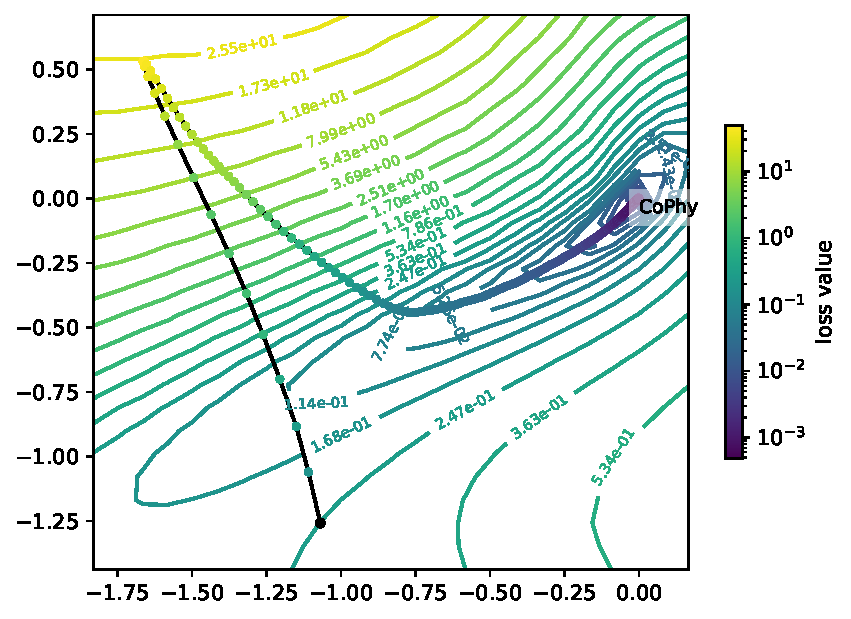
\includegraphics[width=\textwidth]{figures/round3/Cophy_PCA/directions.h5_proj_cos_phy_total.h5_total_phy_loss_2dcontour_proj.pdf}
                \caption{PCA}
                \label{fig:PCAvsAE_outPCA}
                % \caption{PCA}
              \end{subfigure}
              \hfill
             \begin{subfigure}[b]{0.3\textwidth}
                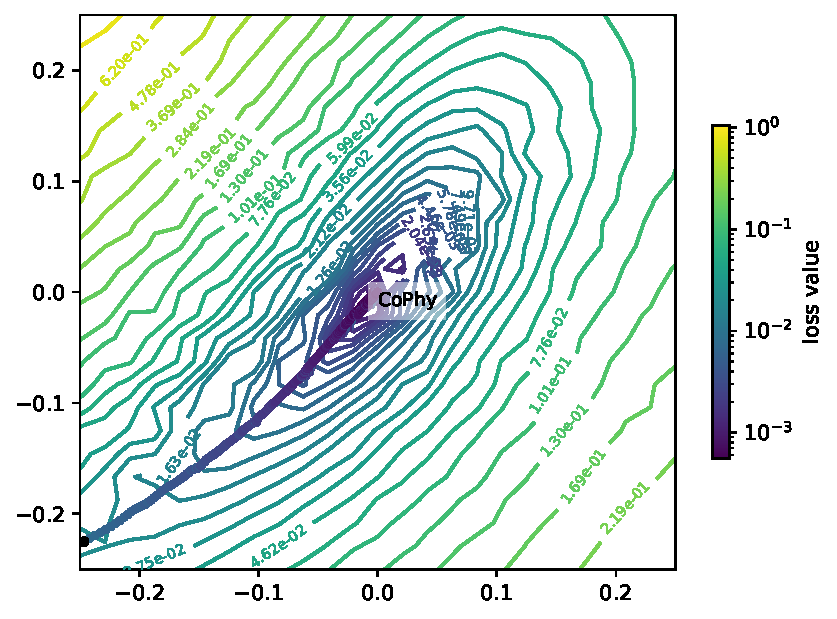
\includegraphics[width=\textwidth]{figures/round3/Cophy_PCA_zoomed/cophyzoomedfixed.pdf}
                \caption{PCA (zoomed-in)}
                \label{fig:PCAvsAE_zoomedPCA}
              \end{subfigure}
              \hfill
              \begin{subfigure}[b]{0.3\textwidth}
                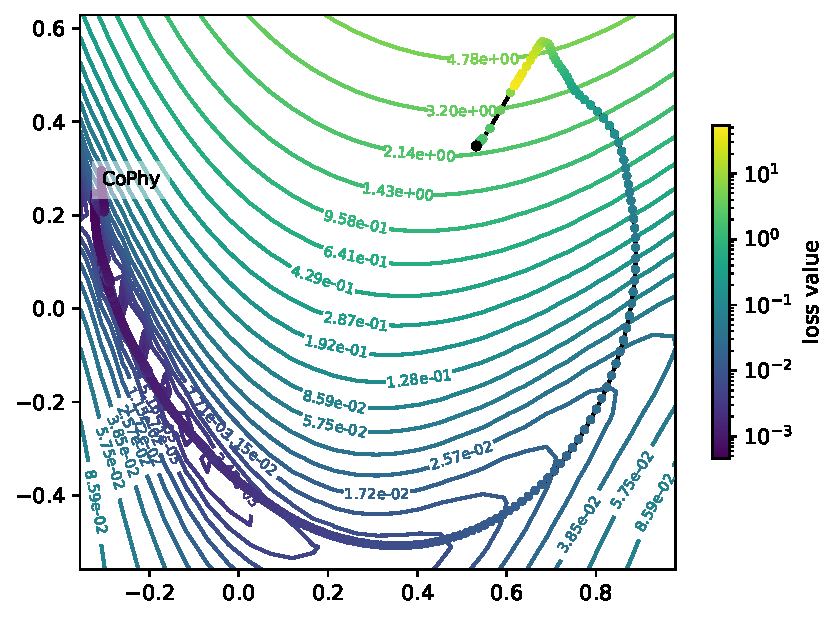
\includegraphics[width=\textwidth]{figures/round3/Kernel-PCA/map_phy_total_loss.pdf}
                % \caption{\proposedautencoder{}}
                \caption{Kernel-PCA}
             \label{fig:KernelPCAloss}
              \end{subfigure}
              \begin{subfigure}[b]{0.3\textwidth}
                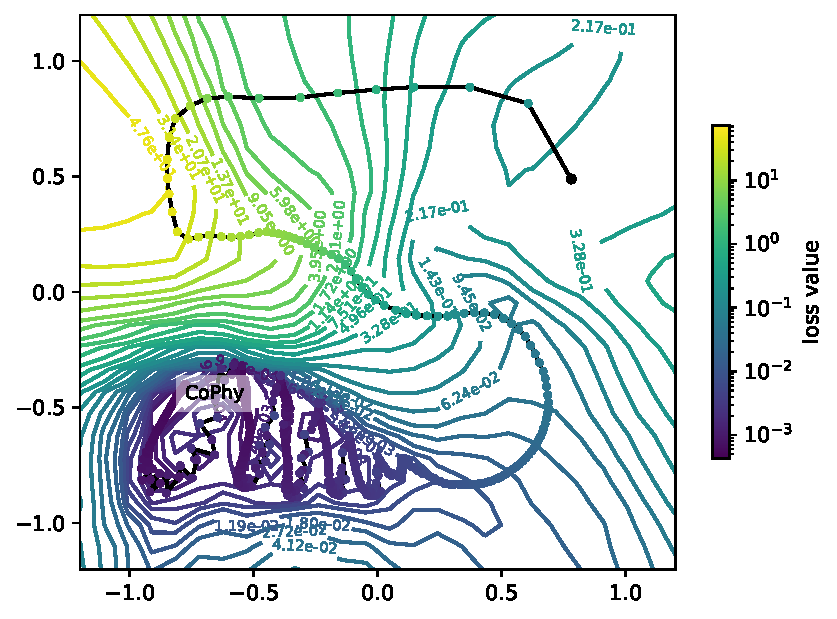
\includegraphics[width=\textwidth]{figures/round3/Cophy_NV/map_phy_total_loss.pdf}
                % \caption{\proposedautencoder{}}
                \caption{\proposedautencoder{}}
             \label{fig:PCAvsAE_out}
              \end{subfigure}
              \hfill
               % \vspace{1cm}
              % \hfill
              \begin{subfigure}[b]{0.33\textwidth}
                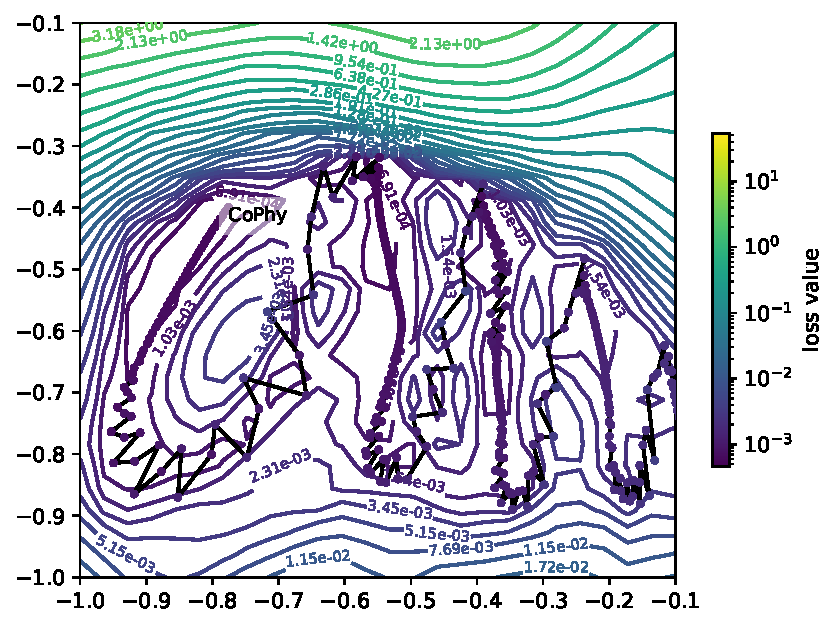
\includegraphics[width=\textwidth]{figures/round3/Cophy_NV_zoomed/map_phy_total_loss.pdf}
                \caption{\proposedautencoder{} (zoomed-in)}
                \label{fig:PCAvsAE_zoomed}
              \end{subfigure}
              \hfill
                \begin{subfigure}[b]{0.3\textwidth}
                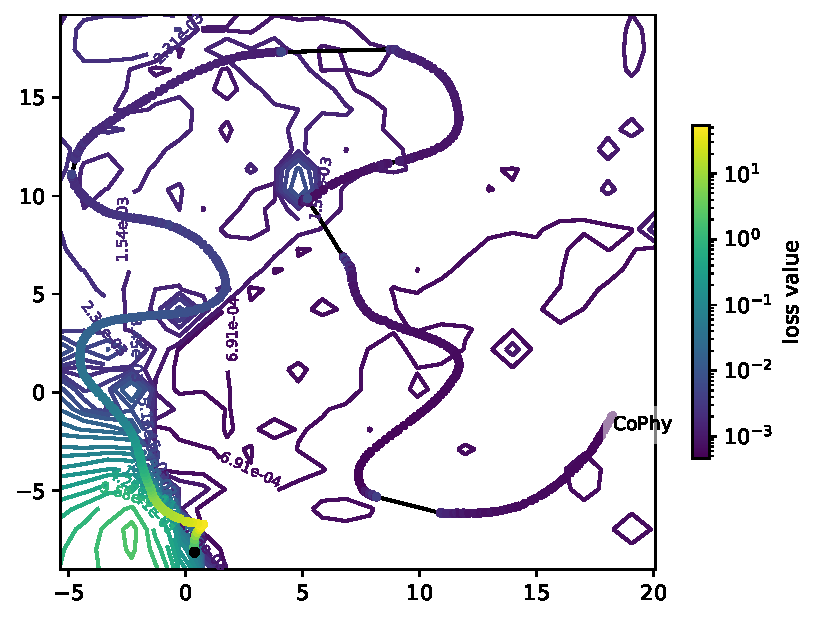
\includegraphics[width=\textwidth]{figures/round3/UMAP/map_phy_total_loss.pdf}
                \caption{UMAP}
                \label{fig:UMAPloss}
                % \caption{PCA}
              \end{subfigure}

             
              \caption{A comparison of \proposedautencoder{} and other baselines in terms of the consistency of \cophy{}'s overall physics loss values between trajectory models and their corresponding manifold projections. 
              %The bottom row is a zoomed-in view of the top one. 
              Clearly, \proposedautencoder{} shows richer details and a manifold that better fits the trajectory models.}
              \label{fig:PCAvsAE}
            \end{figure*}




          To compare \proposedautencoder{} to other non-linear methods, we visualize the same trajectory using UMAP \cite{mcinnes2018umap} and Kernel-PCA \cite{10.1007/BFb0020217} with an RBF kernel in 
          %We choose these methods specifically because, unlike most non-linear dimensionality reduction methods, they have an inverse transform (i.e., they allow for projecting back from the low-dimensional space to the original high-dimensional space). This property is important as we are interested in plotting the trajectory models within the context of a grid that represents a manifold. 
          \cref{fig:PCAvsAE}. Compared to \proposedautencoder{}, we make two observations. First, UMAP uses almost the entire grid to show the local minima at which the model arrives, with little attention to the initial stage of optimization. Thus, UMAP fails to give the full picture of the training trajectory when compared to \proposedautencoder{}. Similarly, while Kernel-PCA is a non-linear method, its landscape visualization looks too simplistic with little insight to provide beyond that of PCA's. 
                    \cref{app:errors_cophy} provides more visualizations on the projection and loss errors of \proposedautencoder{} compared to the other baselines. For a more quantitative assessment, however, we provide some comparative metrics in \cref{tab:quant_losslandscape}. By looking at both the average relative error in loss values and the average projection error in the parameter space, we can see that \proposedautencoder{} beats all the other methods by orders of magnitude.
          %Lastly, looking at the last two rows of \cref{fig:UMAPKernelPCA}, it is obvious that, similar to PCA's case in \cref{fig:PCAvsAE2}, neither UMAP nor Kernel-PCA result in a manifold that fits the trajectory models well.

            %    \begin{figure}[ht]
            %   \centering
            %   \begin{subfigure}[b]{0.33\textwidth}
            %     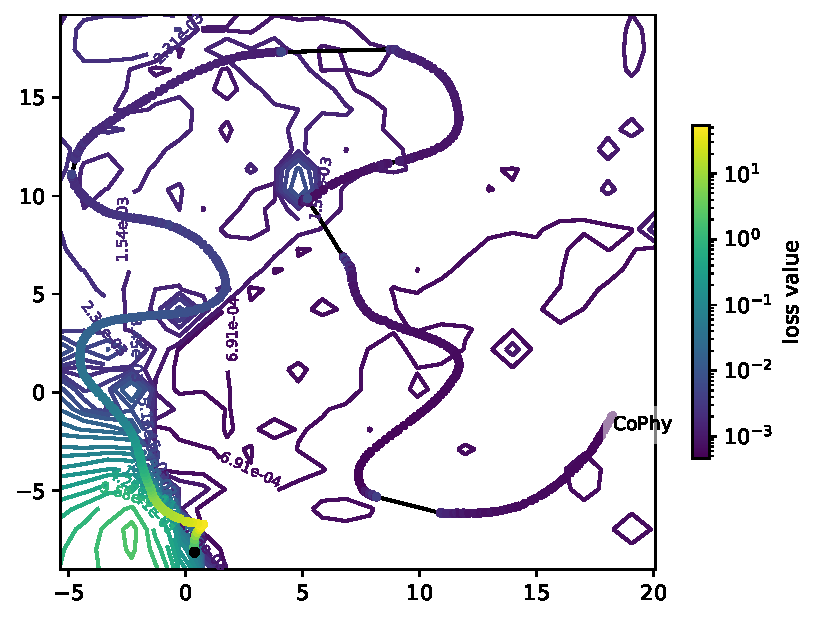
\includegraphics[width=\textwidth]{figures/round3/UMAP/map_phy_total_loss.pdf}
            %     \caption{UMAP}
            %     \label{fig:UMAPloss}
            %     % \caption{PCA}
            %   \end{subfigure}
            %   % \hfill
            %   \begin{subfigure}[b]{0.33\textwidth}
            %     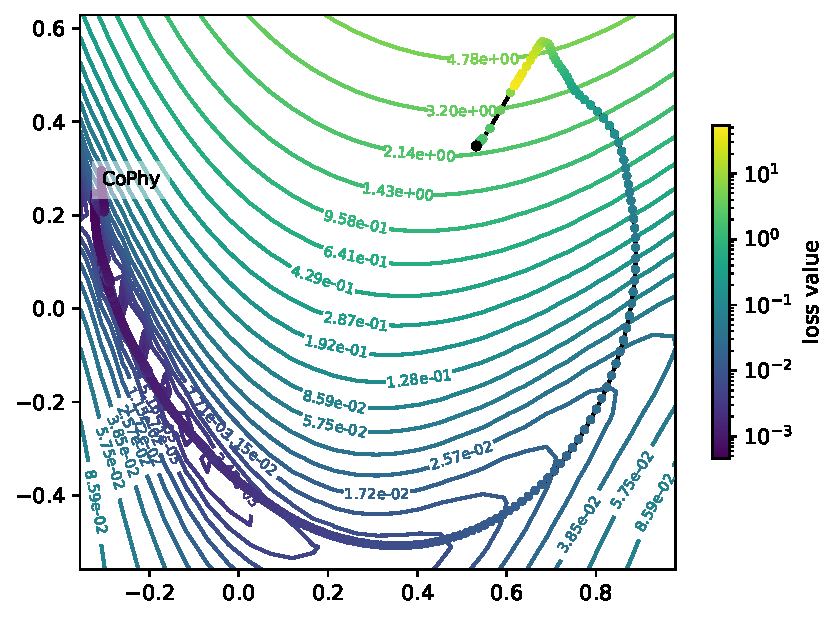
\includegraphics[width=\textwidth]{figures/round3/Kernel-PCA/map_phy_total_loss.pdf}
            %     % \caption{\proposedautencoder{}}
            %     \caption{Kernel-PCA}
            %  \label{fig:KernelPCAloss}
            %   \end{subfigure}
            %     % \caption{A visualization of UMAP and Kernel-PCA in terms of consistency w.r.t \cophy{}'s $\text{Train-MSE}$ loss values between the trajectory and the grid}
            %     % \label{fig:UMAPKernelPCA}

            %   % \centering
            %   % \begin{subfigure}[b]{0.45\textwidth}
            %   %   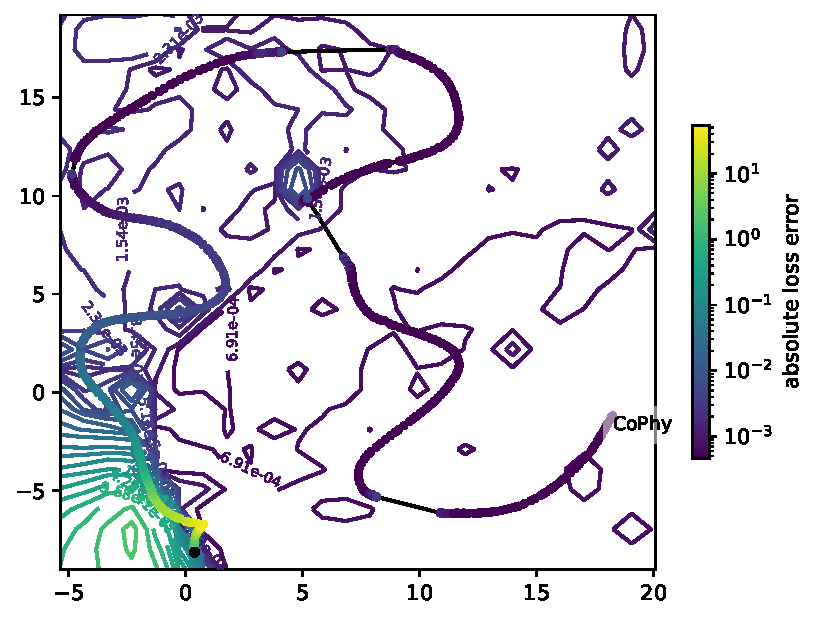
\includegraphics[width=\textwidth]{figures/round3/UMAP/map_phy_total_abs_error.pdf}
            %   %   % \caption{Caption for image 1}
            %   %   % \label{fig:subfig1}
            %   % \end{subfigure}
            %   % \hfill
            %   % \begin{subfigure}[b]{0.45\textwidth}
            %   %   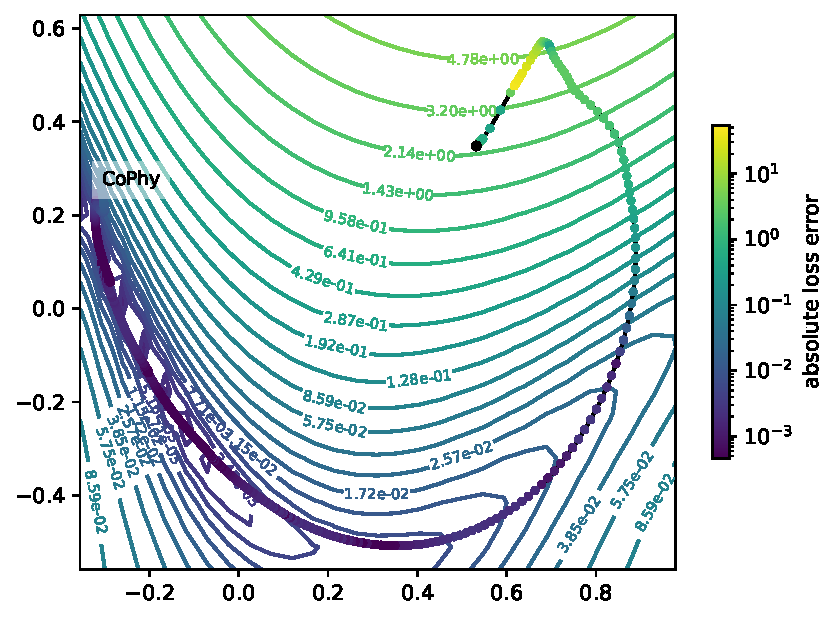
\includegraphics[width=\textwidth]{figures/round3/Kernel-PCA/map_phy_total_abs_error.pdf}
                
            %   % \end{subfigure}
            
            %   %       % \vspace{1cm}
         
            %   % \begin{subfigure}[b]{0.45\textwidth}
            %   %   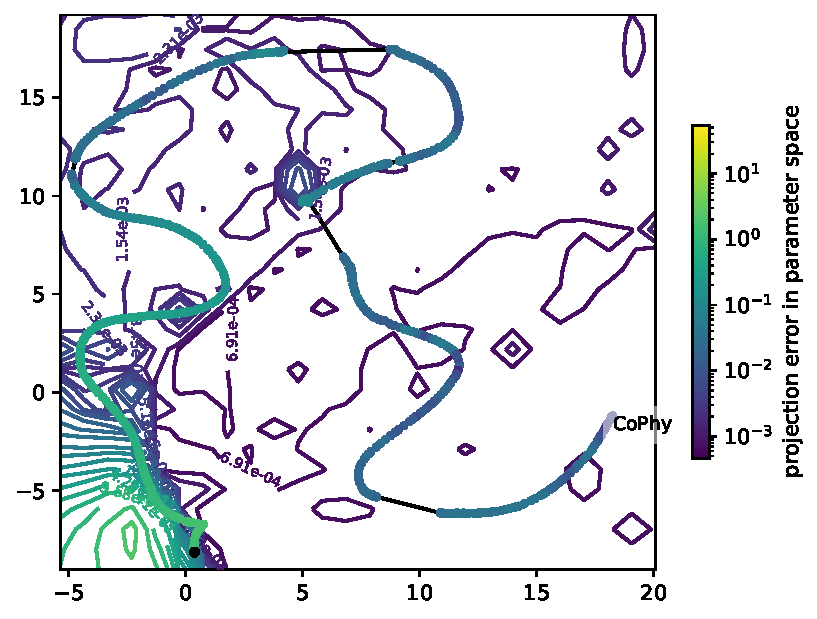
\includegraphics[width=\textwidth]{figures/round3/UMAP/map_phy_total_dists_param_space.pdf}
            %   %   \caption{UMAP}
            %   %   % \label{fig:subfig1}
            %   % \end{subfigure}
            %   % \hfill
            %   % \begin{subfigure}[b]{0.45\textwidth}
            %   %   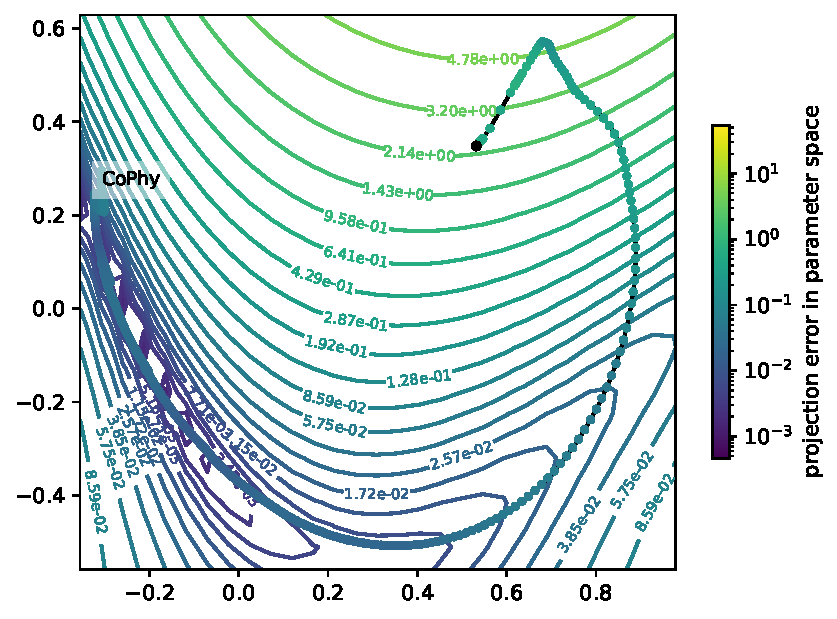
\includegraphics[width=\textwidth]{figures/round3/Kernel-PCA/map_phy_total_dists_param_space.pdf}
            %   %   \caption{Kernel-PCA}
            %     % \label{fig:subfig2}
            %   % \end{subfigure}

            %   \caption{A comparison of UMAP and Kernel-PCA in terms of the consistency of \cophy{}'s total physics loss values between trajectory models and their corresponding manifold projections. Compared to \cref{fig:PCAvsAE}, neither UMAP nor Kernel-PCA look favorable against \proposedautencoder{}. 
            %   }
            %   \label{fig:UMAPKernelPCA}
            % \end{figure}


          
            % \begin{table}
            % \centering
            % % \resizebox{\textwidth}{!}{
            % \begin{tabular}{|c|p{2.5cm}|p{2.5cm}|}
            % \hline
            % \textbf{Method} & \textbf{Average relative physics loss error} & \textbf{Average projection error} \\
            % \hline
            % \proposedautencoder{} & 0.0095 & 0.0005 \\
            % \hline
            % PCA & 1.6782 & 0.2832 \\
            % \hline
            % Kernel-PCA & 4.7250 & 0.0865 \\
            % \hline
            % UMAP & 0.4295 & 0.2307 \\ 
            % \hline
            % \end{tabular}
            % % }
            % \caption{A quantitative comparison of \proposedautencoder{} against other baselines. \proposedautencoder{} outperforms all other baselines across the board.}
            % \label{tab:quant_losslandscape}
            % \end{table}


            \begin{table}
            \centering
            % \resizebox{\textwidth}{!}{
            \begin{tabular}{|p{1cm}|p{1.5cm}|c|p{1cm}|c|}
            \hline
            \textbf{Metric} & \proposedautencoder{}& PCA & Kernel-PCA & UMAP   \\
            \hline
            \textbf{$e_{\text{relative}}$} & 0.0095 & 1.6782  & 4.7250 & 0.4295\\
            \hline
            \textbf{$e_{\text{proj}}$} & 0.0005 &  0.2832 & 0.0865 & 0.2307 \\
            % \hline
            % Kernel-PCA &  & \\
            % \hline
            % UMAP &  &  \\ 
            \hline
            \end{tabular}
            % }
            \caption{A quantitative comparison of \proposedautencoder{} against other baselines in terms of average relative physics loss error \textbf{$e_{\text{relative}}$} and average projection error \textbf{$e_{\text{proj}}$}. \proposedautencoder{} outperforms all other baselines across the board.}
            \label{tab:quant_losslandscape}
            \end{table}

          \subsubsection{Using \proposedautencoder{} to Study the Advantages of the \cophy{} Approach.} 
          % After demonstrating \proposedautencoder{}'s advantages , 
          We here show \proposedautencoder{}'s usefulness for comparing different models by plotting the trajectories of \cophy{} and its baseline \nn{} in \cref{fig:NNcophylandscape}. Both trajectories start from the same model initialization (marked with a thick border). The top two sub-figures use PCA to visualize $\text{Test-MSE}$ and the spectrum loss, \eloss{}, which is one of the two physics losses used to train the model. 
          %\eloss{} and \nsloss{}. 
          The bottom two sub-figures show the corresponding loss landscapes for \proposedautencoder{}. We notice that %in \ref{ss:proposedvsbaselines}
          % \begin{enumerate}
          % \item \textbf{\proposedautencoder{} successfully captures all critical points of interest:} 
          %Since its plane only passes through the last model of \cophy{}'s trajectory, 
          PCA utterly fails at capturing \nn{}'s critical points. In \cref{fig:elossPCA}), 
          %This is especially obvious in  where 
          PCA not only misses \nn{}'s minima, but also shows inconsistency in its loss values (i.e., the model colors indicate that it is descending, while the contours indicate the opposite). This is in contrast to \proposedautencoder{}, where \nn{}'s and \cophy{}'s minima is distinctly visualized with high consistency in terms of loss values. %Another crucial difference is that looking at Fig. \ref{fig:elossboth}, it is clear that \cophy{} focuses first on optimizing \eloss{}. This happens even at the cost of increasing  both \nsloss{}, and $\text{Test-MSE}$ at first. Only later do \nsloss{}, and $\text{Test-MSE}$ decrease. This story fits with the theme of annealing \eloss{} and cold starting \cophy{}, which was explained in Section \ref{ss:cophy}. On the other hand, the same story does not check through the PCA lens in the right column.
          % \item \textbf{\proposedautencoder{} successfully captures gradient descent:} Looking at \cref{subfig:pcatest}, PCA \nn{} gives the false impression that \nn{} ends up somewhere in a concavity but does not follow its gradient towards the minima at the final epochs of the optimization process, even though it is not influenced by any loss terms other than the mean-square-error. This contradicts the notion that optimizers such as Stochastic Gradient Descent (SGD) or ADAM roughly follow the direction of the gradient. On the other hand, the trajectory of \nn{} in \cref{subfig:minetest} using \proposedautencoder{} clearly shows that \nn{} ``descends" towards a plateau, where the gradient is weak. This visualization fits with the common conception about gradient-descent-based optimization.
          % \item \textbf{\proposedautencoder{} avoids inconsistency:} 
          Another inconsistency is found by looking at \nn{}'s trajectory in \cref{subfig:pcatest}. Here, PCA shows that it crosses the $2.28\mathrm{e}{-2}$ contour twice, implying that the trajectory descends and then ascends again. This, however, is false as can be verified by looking at the trajectory model colors and how they become darker as the final model is approached, indicating that the loss monotonically decreases. This contradiction leads to confusion
          %Thus, there is an inconsistency in PCA's visualization that leads to confusion. 
          that is not present in \proposedautencoder{}'s case in \cref{subfig:minetest}, making the latter more useful. 
          %Similarly, looking at \nn{}'s trajectory in \cref{fig:elossPCA}, PCA shows that while the trajectory loss values decrease over late epochs, the corresponding contours show an increase in loss values. This inconsistency is confusing and undermines the tool's usefulness. On the other hand, \proposedautencoder{} in \cref{fig:elossmine} does not exhibit such an inconsistency, making it more effective and useful than PCA.
          
          % \end{enumerate}
                     
               \begin{figure}[htp]
              \centering
                            % \vspace{-2.5cm}
              %       \begin{subfigure}[b]{0.4\textwidth}
              %   \includegraphics[width=\textwidth]{figures/bothNNCophy2/directions.h5_proj_cos_mse_train_loss.h5_train_loss_mse_loss_2-Dcontour_proj.pdf}
              %   \caption{PCA - $\text{Train-MSE}$ }
              % \end{subfigure}
              % \hfill
              % \begin{subfigure}[b]{0.4\textwidth}
              %   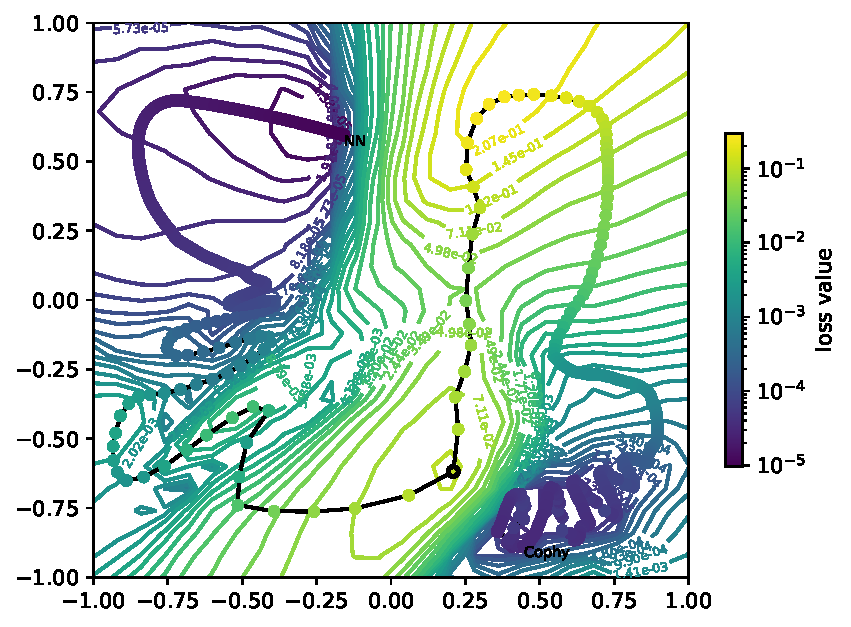
\includegraphics[width=\textwidth]{figures/bothNNCophy2/map_mse_train_loss_loss.pdf}
              %   \caption{\proposedautencoder{} - $\text{Train-MSE}$ }
              %   \label{fig:elossboth}
              % \end{subfigure}
            % \vspace{1cm}
         

              \begin{subfigure}[b]{0.3\textwidth}
                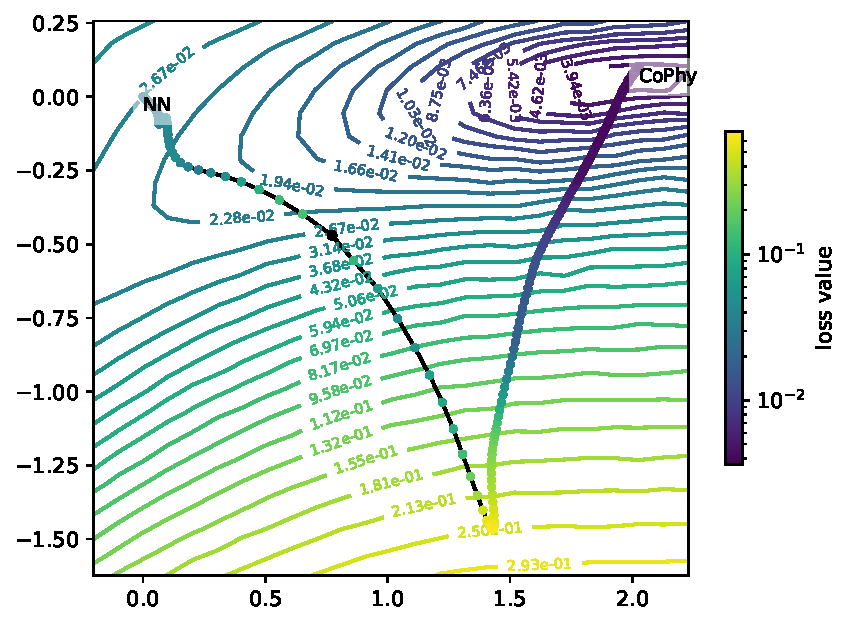
\includegraphics[width=\textwidth]{figures/round3/both_PCA/directions.h5_proj_cos_mse_test_loss.h5_test_loss_mse_loss_2dcontour_proj.pdf}
                \caption{PCA - $\text{Test-MSE}$ }
                \label{subfig:pcatest}
              \end{subfigure}
              % \hfill
            \begin{subfigure}[b]{0.3\textwidth}
                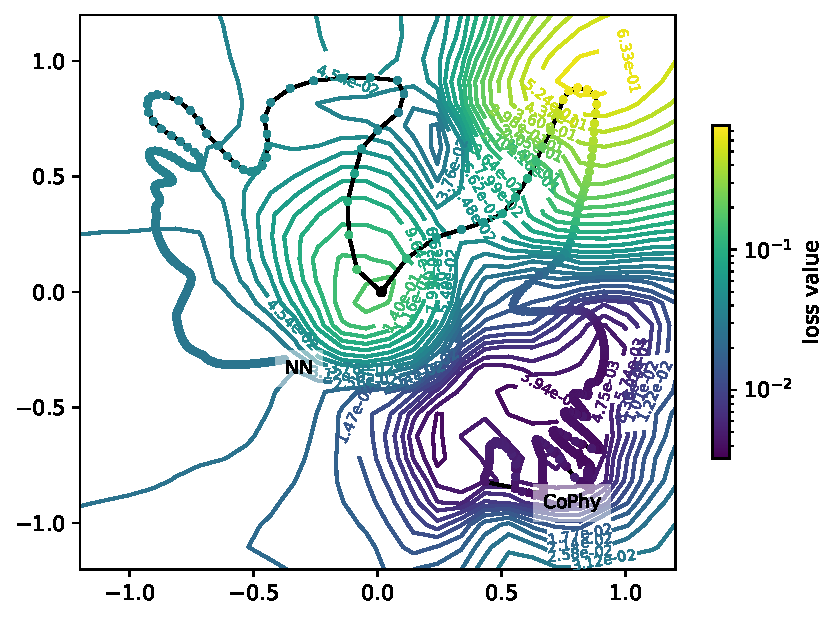
\includegraphics[width=\textwidth]{figures/round3/both_NV/map_mse_test_loss_loss.pdf}
                \caption{\proposedautencoder{} - $\text{Test-MSE}$ }
                % \label{fig:subfig1}
                \label{subfig:minetest}
              \end{subfigure}

                    % \vspace{1cm}
         
              \begin{subfigure}[b]{0.3\textwidth}
                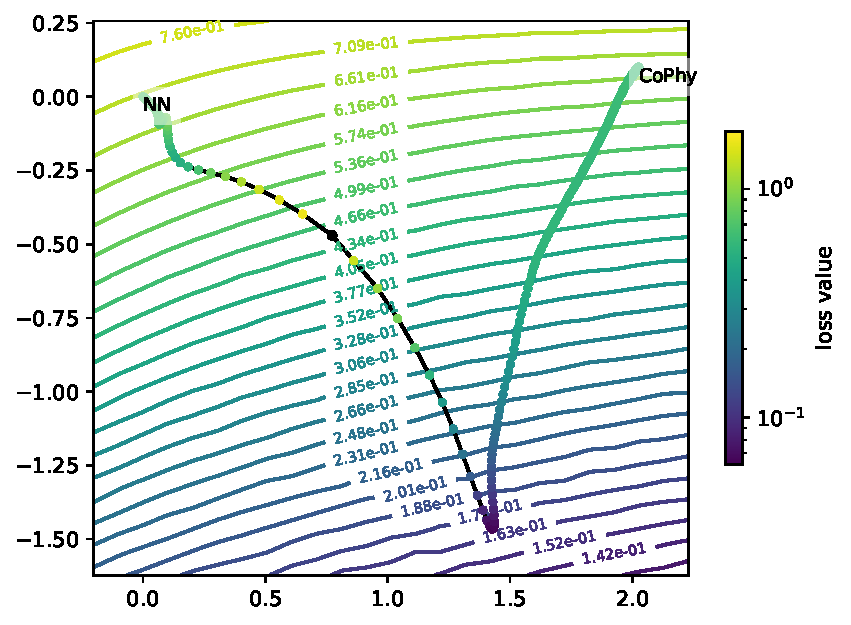
\includegraphics[width=\textwidth]{figures/round3/both_PCA/directions.h5_proj_cos_e_total.h5_total_e_loss_2dcontour_proj.pdf}
                \caption{PCA - $\eloss{}$ }
                \label{fig:elossPCA}
              \end{subfigure}
              % \hfill
              \begin{subfigure}[b]{0.3\textwidth}
                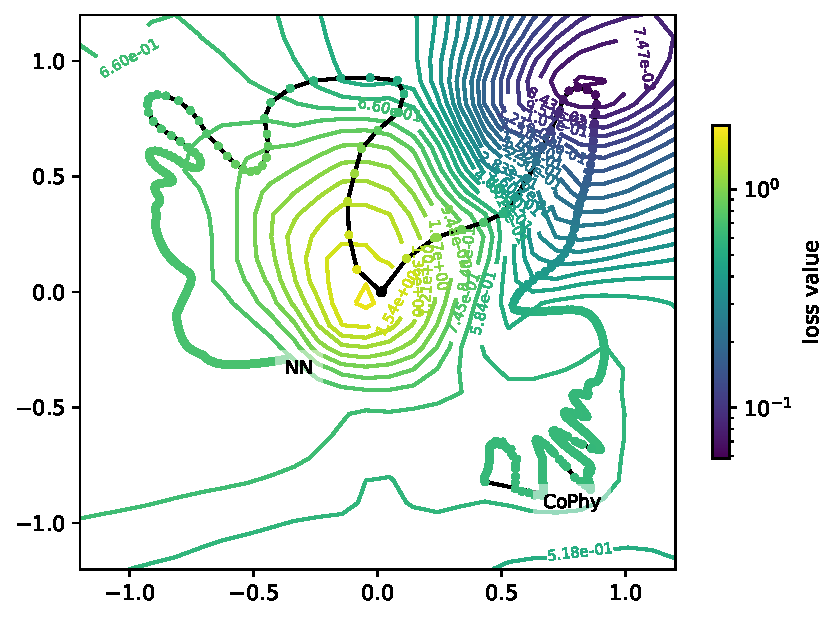
\includegraphics[width=\textwidth]{figures/round3/both_NV/map_e_total_loss.pdf}
                \caption{\proposedautencoder{} - $\eloss{}$  }
                \label{fig:elossmine}
              \end{subfigure}
         
              % \begin{subfigure}[b]{0.45\textwidth}
              %   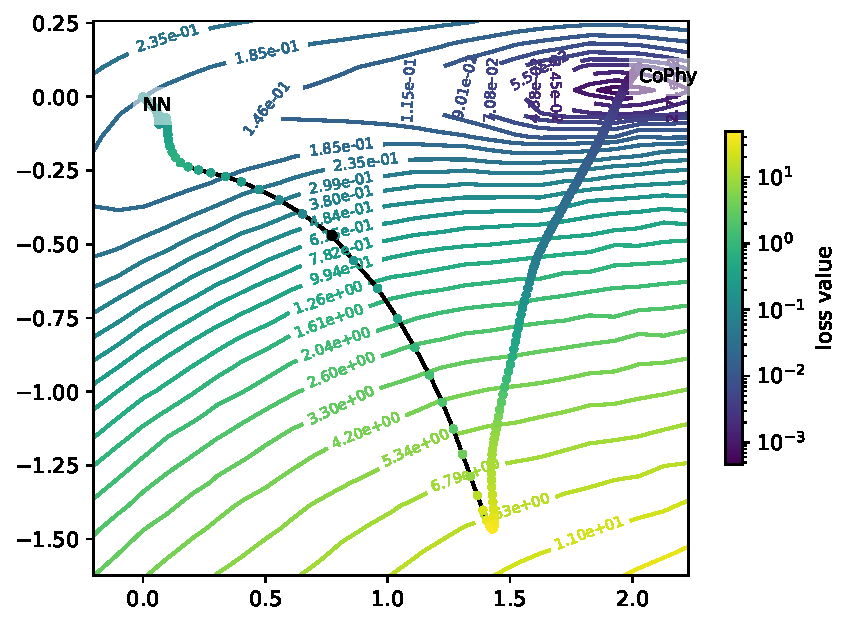
\includegraphics[width=\textwidth]{figures/round3/both_PCA/directions.h5_proj_cos_phy_total.h5_total_phy_loss_2dcontour_proj.pdf}
              %   \caption{PCA - $\nsloss{}$ }
              %   % \label{fig:subfig1}
              % \end{subfigure}
              % \hfill
              % \begin{subfigure}[b]{0.45\textwidth}
              %   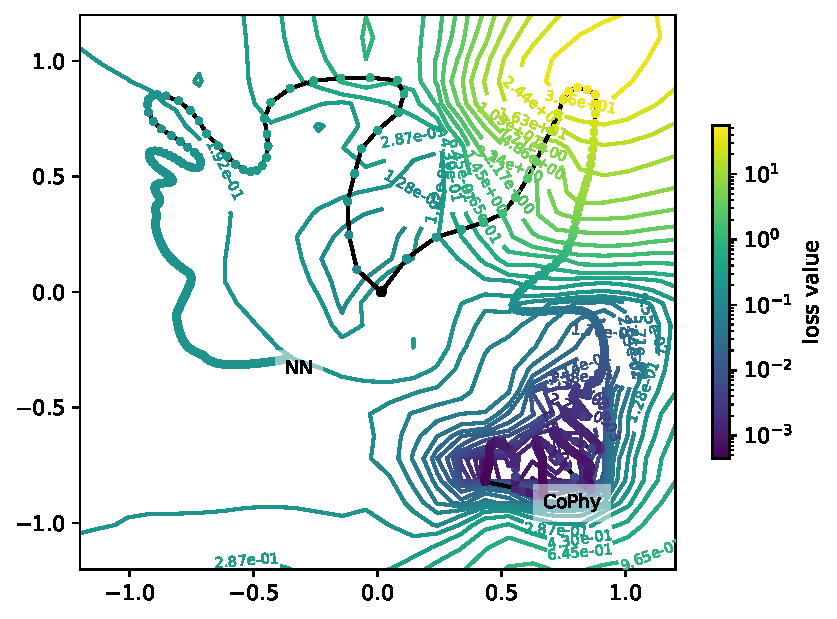
\includegraphics[width=\textwidth]{figures/round3/both_NV/map_phy_total_loss.pdf}
              %   \caption{\proposedautencoder{} - $\nsloss{}$  }
              %   % \label{\proposedautencoder{}}
              % \end{subfigure}
              
              \caption{The loss landscapes of \cophy{} and \nn{} for different loss terms using PCA and \proposedautencoder{}. Comparing the two, it is clear that \proposedautencoder{} tells a more accurate and insightful story.}
              \label{fig:NNcophylandscape}
            \end{figure}

          

            
                        % \paragraph{Investigating Physics-Guided Optimization Using \proposedautencoder{}} 
            %\label{ss:landscapefuture}

       

                 % This is especially the case since, to the best of my knowledge, there has been very little investigation of the effects of \SGML{} by means of landscape visualization (e.g., whether \SGML{} models have simpler or more complex loss surfaces, and whether their minima are sharp or flat). 

                %Using landscape visualization, however, Section \ref{ss:cophy_landscape} demonstrated that the proper use of \SGML{} helps improve model performance by reaching minima with better generalizability. Here, I apply similar analyses to another benchmark problem in physics: Partial Differential Equations (PDE) solving using \SGML{} \cite{raissi2019physics, YANG2019136, GAO2021110079, JIN2021109951, QRESNET}. More specifically, I choose to use Physics Informed Neural Networks (PINNs) \cite{raissi2019physics}, which are a popular type of \SGML{} to illustrate the usefulness of my proposed method.
                %For example, there has recently been a significant amount of literature on using \SGML{} for solving partial differential equations (PDEs) \cite{raissi2019physics, YANG2019136, GAO2021110079, JIN2021109951, QRESNET}, such as Burgers', Darcy's, and Navier-Stokes equations. 
                % One of the quite few examples that show the importance of using the landscape visualization tool within the \SGML{} frame can be demonstrated by considering training Physics Informed Neural Networks (PINNs) \cite{raissi2019physics}. 
                
                 % These domains are fertile ground for understanding the effect of different architectural decisions and hyper-parameters, especially those inspired by \SGML{}, on the optimization process and model quality. 

                 
                 % For example, Krishnapriyan et. al. \cite{krishnapriyan2021characterizing} use landscape visualizations to demonstrate the challenge of optimizing PINNs, and to study how tuning the regularization parameter leads to a trade-off between difficulty of optimization and poor generalization. 
                 %However, their work is specific to PINNs and limited to a single parameter, leaving much to be explored in terms of the \SGML{} framework in general. Such a research gap poses a great opportunity to make \SGML{} research more informed and interpretable.
                
         
            
                
                %To that end, I extend my work in two directions:



           % \paragraph{Investigating Physics Loss Balancing in \SGML{} Using \proposedautencoder{}} 

           \subsection{Applying \proposedautencoder{} on PINNs} 

            % Having sufficiently demonstrated \proposedautencoder{}'s advantages over other linear and non-linear baselines in \cref{ss:cophy_landscape2}, 
            We here explore \proposedautencoder{}'s usefulness in studying Physics-Informed Neural Networks (PINNs), which have been widely and successfully used by many researchers in recent years to solve partial differential equations (PDEs), which appear in many real-world engineering and scientific applications. Moreover, PINNs present themselves as a convenient test-bed for our proposed landscape visualization method, thanks to 
            %the multitude of existing PINN models, the plethora of PDEs, and 
            the significant effect of varying optimization hyper-parameters on PINN performance.

            For training PINNs, the loss terms that play a role  
            %in this framework 
            are the residual loss $\lres$, the initial condition loss $\lic$, and the boundary condition loss $\lbc$. The total loss being optimized is:
            \begin{equation}
                \text{L}_{total} = \cres \times \lres + \cic \times \lic + \cbc\times  \lbc.
            \end{equation}
            See \cref{app:pdes} for a detailed literature review on PINNs.



        \subsubsection{Demonstrating \proposedautencoder{}'s Flexibility With Different Constraints.} \label{ss:constraints}
        As discussed in \cref{se:constaints}, one of \proposedautencoder{}'s advantages is its ability to warp the learned manifold to satisfy certain constraints. To demonstrate this, we use PINN for the Convection equation as a target application. We set $\beta=30$, a high value, making the PDE harder to solve 
        %(see \cref{app:pdes} for more details). This creates a 
        and the loss landscape more complex and interesting to visualize (see \cref{app:pdes} for details).
        %that is more complex, riddled with non-convexities, and harder to optimize. Such a landscape would be interesting to visualize.

        \cref{fig:constraints} shows a progression of \proposedautencoder{} models visualizing $\ltest$  (i.e., the prediction error at test domain points) of the same PINN model. However, these \proposedautencoder{} models are trained with different constraints. First, \cref{fig:constraintsvanilla} shows the loss landscape with no constraints. Subsequent sub-figures show the different manifolds obtained by varying the \proposedautencoder{}'s training constraints.
        %, or a combination of constraint and comment on the resulting landscape visualization.
        % After the ``vanilla" landscape shown in \cref{fig:constraintsvanilla}, 
        \cref{fig:constraintspolar} uses ${\lanch}_1$. As a result, the trajectory stretches almost perfectly across the grid between two opposite corners. 
        %However, we notice that the steps on the trajectory are not equi-distant \underline{in the grid space}. As such a property maybe desired (see \cref{p:trajscaling}), we add a second constraint, $\ltraj$. \cref{fig:constraintsequipolar} shows a trajectory that simultaneously stretches between the two corners and has equi-distant steps in the grid space. 
        Alternatively, to show the effect of $\lgrid$, 
        %we exper combine it with $\lanch_2$. 
        we use a large $\lmax=8$ to impose high grid density at the vicinity of the trajectory models. As expected, \cref{fig:constraintgrid} shows a grid that zooms almost entirely onto
        %space around the last stage of model optimization (i.e., near the grid center) 
        the vicinity of the trajectory, highlighting more details of that area compared to the previous sub-figures.

                        
        \begin{figure*}[htb]
              \centering
              \begin{subfigure}[b]{0.3\textwidth}
                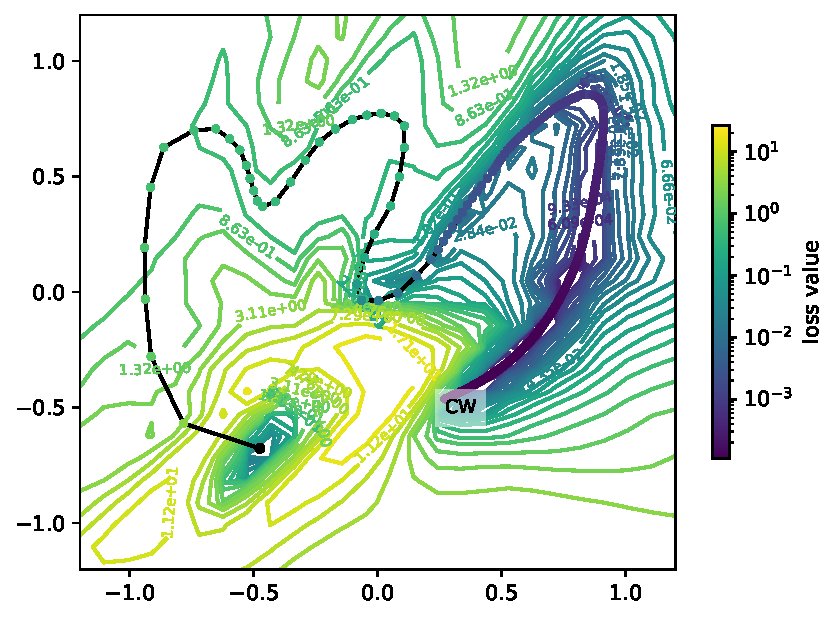
\includegraphics[width=\textwidth]{figures/round3/vanilla/map_residual_train_loss_loss.pdf}
                \caption{vanilla}
                \label{fig:constraintsvanilla}
              \end{subfigure}
              \hfill
            \begin{subfigure}[b]{0.3\textwidth}
                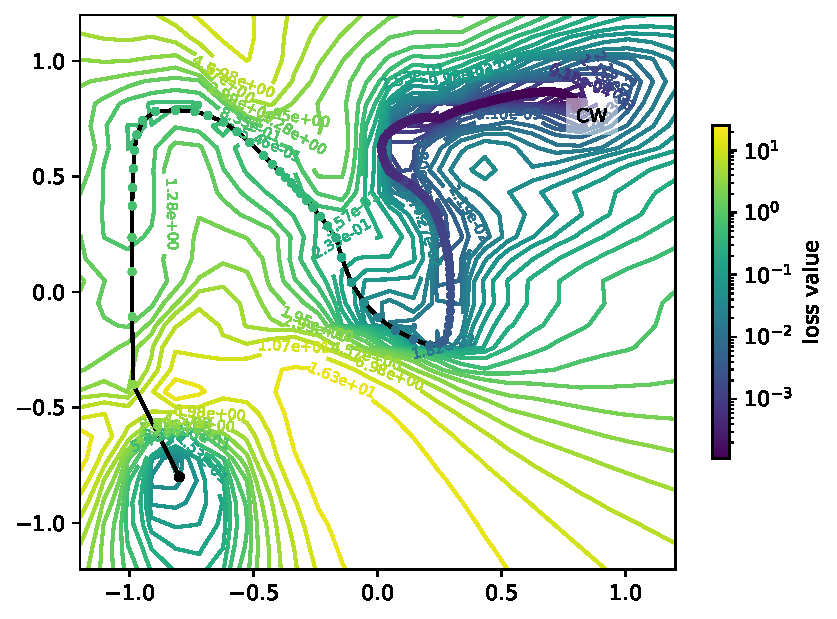
\includegraphics[width=\textwidth]{figures/round3/anch1/map_residual_train_loss_loss.pdf}
                \caption{with ${\lanch}_1$}
                \label{fig:constraintspolar}
              \end{subfigure}
                    % \vspace{1cm}
              % \begin{subfigure}[b]{0.4\textwidth}
              %   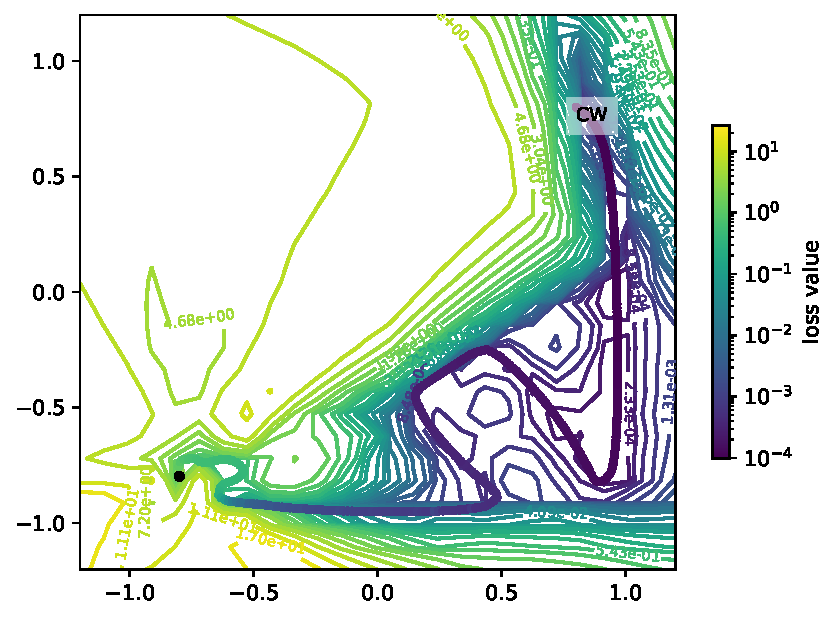
\includegraphics[width=\textwidth]{figures/round3/anch1equi/map_residual_train_loss_loss.pdf}
              %   \caption{with ${\lanch}_1$ and $\ltraj$}
              %   \label{fig:constraintsequipolar}
              % \end{subfigure}
              \hfill
              \begin{subfigure}[b]{0.3\textwidth}
                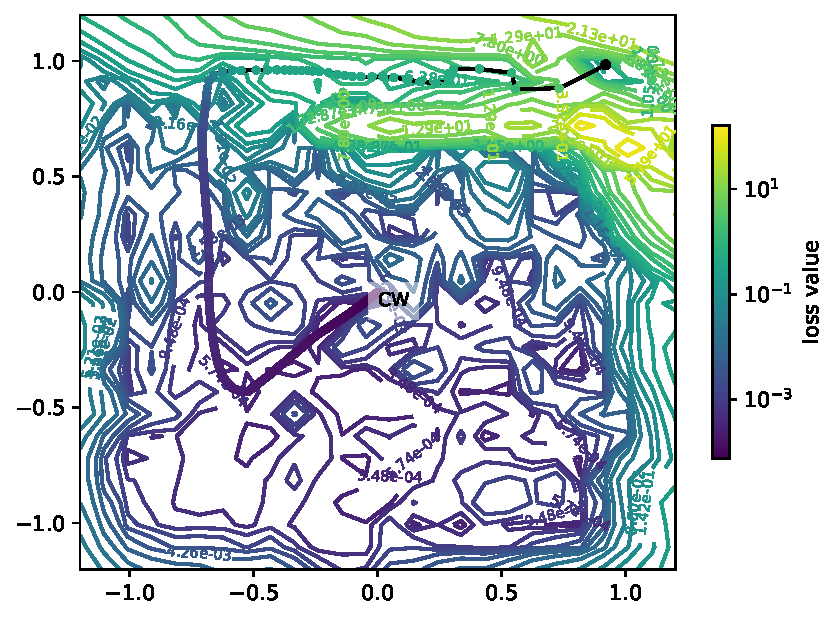
\includegraphics[width=\textwidth]{figures/round3/grid8/map_residual_train_loss_loss.pdf}
                \caption{with ${\lanch}_2$ and $\lgrid$ }
                \label{fig:constraintgrid}
              \end{subfigure}

              \caption{A series of \proposedautencoder{} landscape visualizations of $\lres$ with different constraints. Notice the versatility of the proposed method and its ability to learn the desired manifold by employing appropriate constaints.}
              \label{fig:constraints}
        \end{figure*}

        
        We further study the effect of $\lgrid$ by varying $\lmax$, the hyper-parameter that correlates with the grid density near trajectory models. \cref{fig:Lgrid} shows \underline{the \textit{density} landscape} (i.e., the color-coding indicates grid density and not loss values) for two different values of $\lmax$. 
        %More precisely, at each grid point, the inverse distance density is calculated using the formula:
        % Instead of Euclidean distances,
        We use a $\text{CKA}$-similarity-based density that is defined as:

        % \begin{equation}
        %     \rho_{m \in \gridpoints} = \sum_{m^\prime \in \gridpoints \setminus \{m\}} \frac{1}{d_{m^\prime, m}}
        % \end{equation}

        \begin{equation}
            \rho_{m \in \gridpoints} = \sum_{m^\prime \in \gridpoints \setminus \{m\}} \text{CKA}(m^\prime, m),
        \end{equation}
        %where $d_{m^\prime, m}$ is the distance between two grid points in the parameter space. 
        where $\text{CKA}(m^\prime, m)$ is the $\text{CKA}$ similarity measure between two neural networks as defined in \cite{kornblith2019similarity}.
        % Thus, the more similar a grid point is to the other grid points in the parameter space, the higher the density is at that point in the grid space. 
        As can be seen in \cref{fig:Lgrid}, the density of the grid especially near trajectory models increases with $\lmax$. 
        %Also, while the density is generally highest near the trajectory models, it decreases for farther grid points. 
        This shows that $\lgrid$ can be a vital tool for engineering the manifold visualization through the appropriate choice of $\lmax$.

        \begin{figure}[htb]
          \centering
          % \begin{subfigure}[b]{0.45\textwidth}
          %   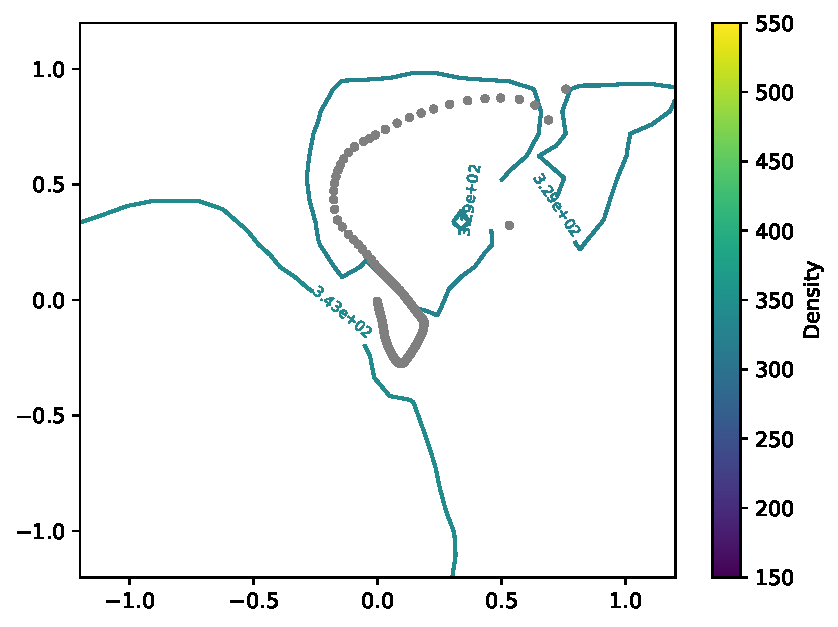
\includegraphics[width=\textwidth]{figures/round3/grid05/map_residual_grid_density.pdf}
          %   \caption{$L=0.5$}
          %   % \label{}
          % \end{subfigure}
          % \hfill
        \begin{subfigure}[b]{0.23\textwidth}
            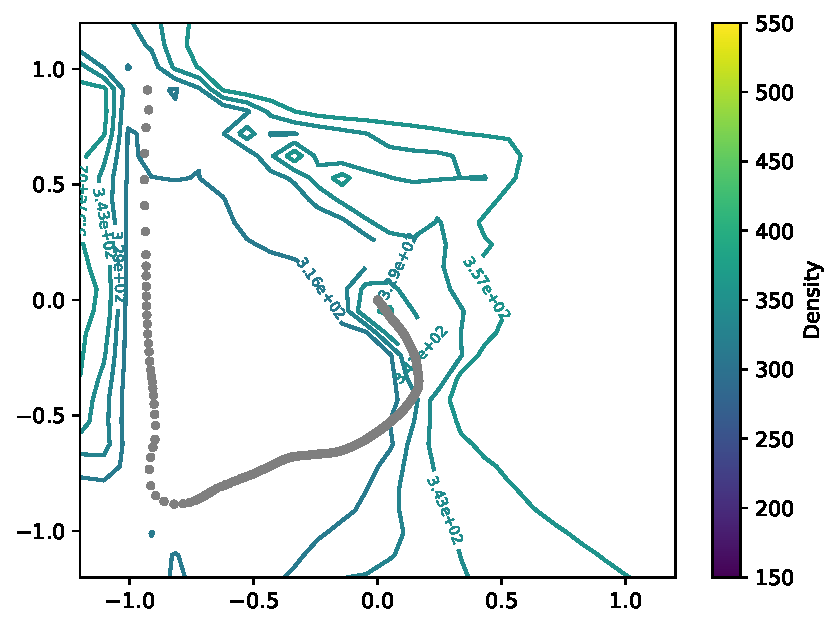
\includegraphics[width=\textwidth]{figures/round3/grid2/map_residual_grid_density.pdf}
            \caption{$L=2$}
            % \label{}
          \end{subfigure}
                % \vspace{1cm}
          % \begin{subfigure}[b]{0.45\textwidth}
          %   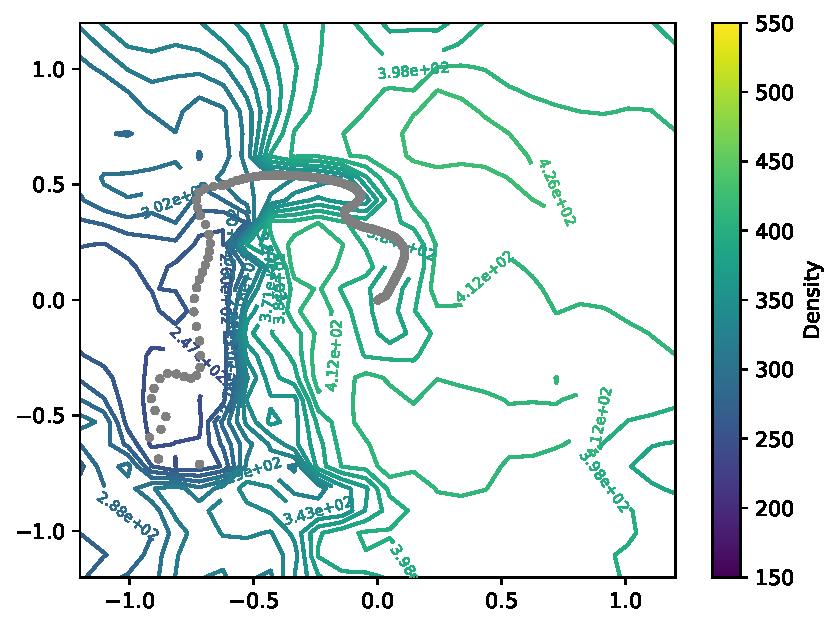
\includegraphics[width=\textwidth]{figures/round3/grid4/map_residual_grid_density.pdf}
          %   \caption{$L=4$}
          %   % \label{}
          % \end{subfigure}
          \hfill
          \begin{subfigure}[b]{0.23\textwidth}
            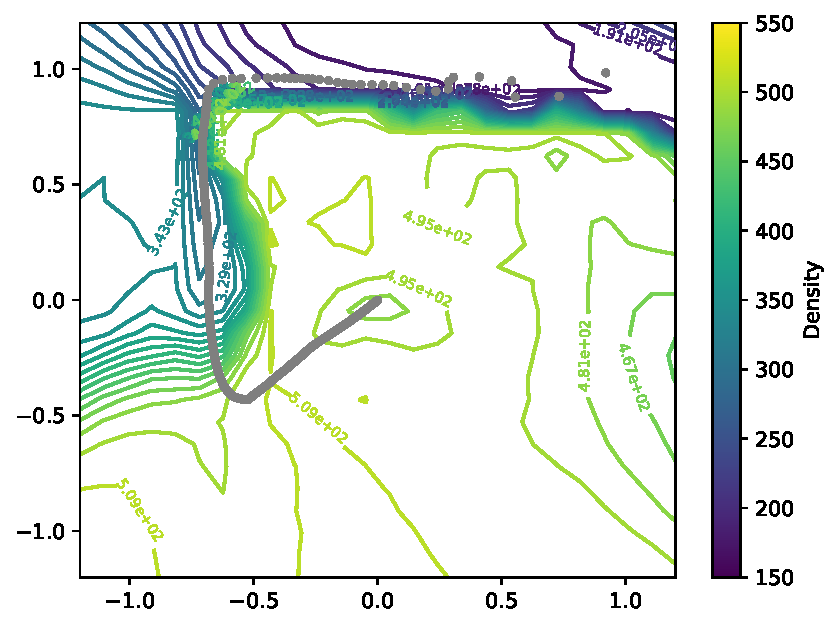
\includegraphics[width=\textwidth]{figures/round3/grid8/map_residual_grid_density.pdf}
            \caption{$L=8$}
            % \label{}
          \end{subfigure}

          \caption{A comparison of two \proposedautencoder{} \textit{density} landscape visualizations as a result of using $\lgrid$ with two different $\lmax$ values. As can be seen, through this constraint, \proposedautencoder{} grants its user greater flexibility to decide the appropriate zooming factor.}
          \label{fig:Lgrid}
        \end{figure}







         \subsubsection{Using \proposedautencoder{} To Study PINNs' Training Pathologies.} \label{ss:NTK}
         Next, we use \proposedautencoder{} to visually verify \cite{wang2020and}'s findings on PINNs through the lens of Neural Tangent Kernel (NTK). In their work, the authors hypothesize that PINN training pathologies result from a discrepancy in the convergence rate of the different loss components. More precisely, they show that the PDE's residual loss ($\lres$) converges faster than the boundary condition loss ($\lbc$), leading to a sub-optimal model. To verify this claim, we train a \proposedautencoder{} to visualize the loss landscape for the two different optimization approaches considered in \cite{wang2020and}. Namely, an approach that trains with constant loss weighting, and another with NTK-based adaptive loss weighting. An ${\lanch}_3$ pinning constraint is imposed to place the models over the perimeter of a circle, making it easy to compare the two approaches. As can be seen in \cref{fig:PINNsNTK}, the authors' claim is easily verifiable using our proposed visualization method. First, in line with the authors' hypothesis, while the terminal $\lres$ and $\lic$ are relatively worse for the NTK-based approach, its terminal $\lbc$ is much better, indicating that an optimal $\lbc$ is essential for obtaining a well-trained PINN. Another observation we make in accordance with their paper is that the NTK-based approach reaches flat minima for all losses at a somewhat similar cadence. This is in contrast to the baseline model where the different losses converge at variable rates, traversing loss landscapes that are less flat and of variable slopes. 


        \begin{figure*}[htb]
            \centering
            
            \begin{subfigure}[b]{0.3\textwidth}
                \centering
                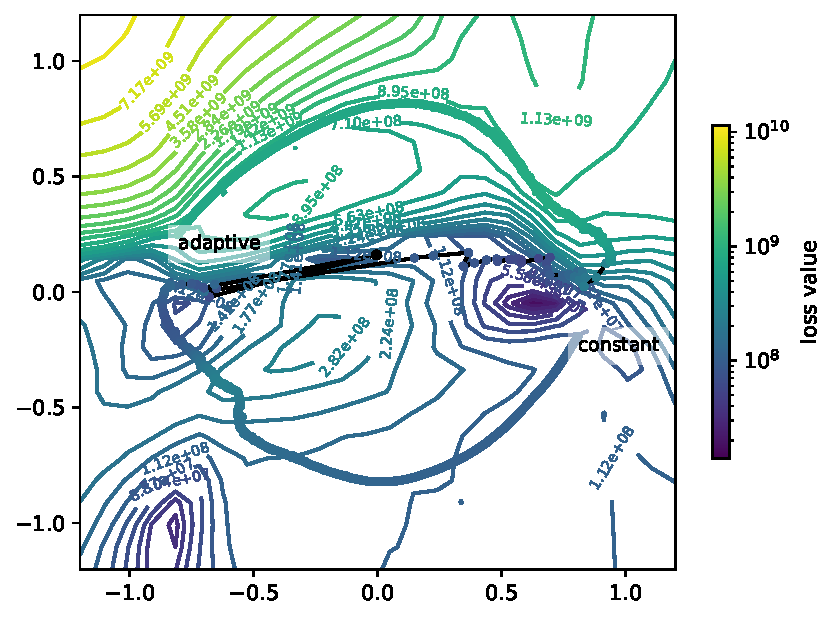
\includegraphics[width=\textwidth]{figures/round3/NTK/map_r_train_loss_loss.pdf}
                \caption{residual loss ($\lres$)}
            \end{subfigure}
            \hfill
            \begin{subfigure}[b]{0.3\textwidth}
                \centering
                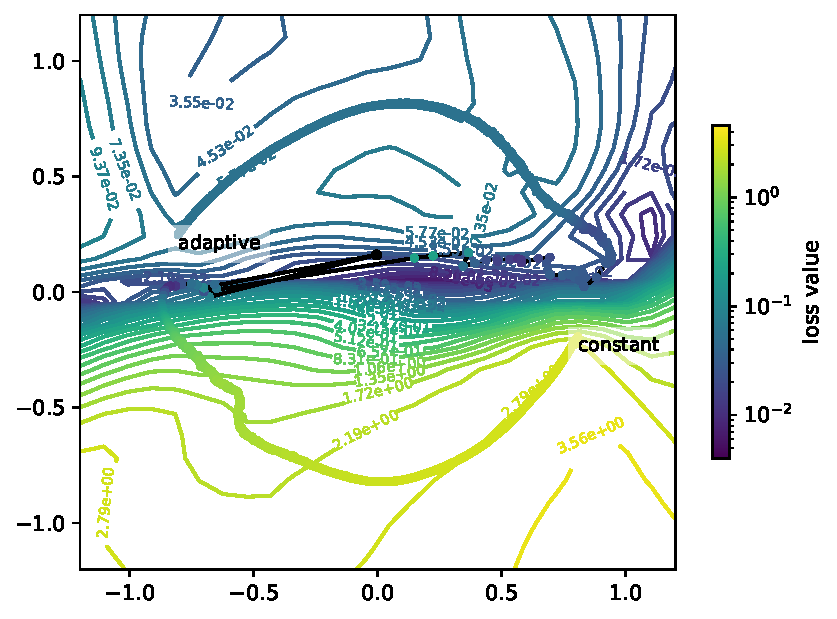
\includegraphics[width=\textwidth]{figures/round3/NTK/map_bc_train_loss_loss.pdf}
                \caption{boundary condition loss ($\lbc$)}
            \end{subfigure}
            \hfill
            \begin{subfigure}[b]{0.3\textwidth}
                \centering
                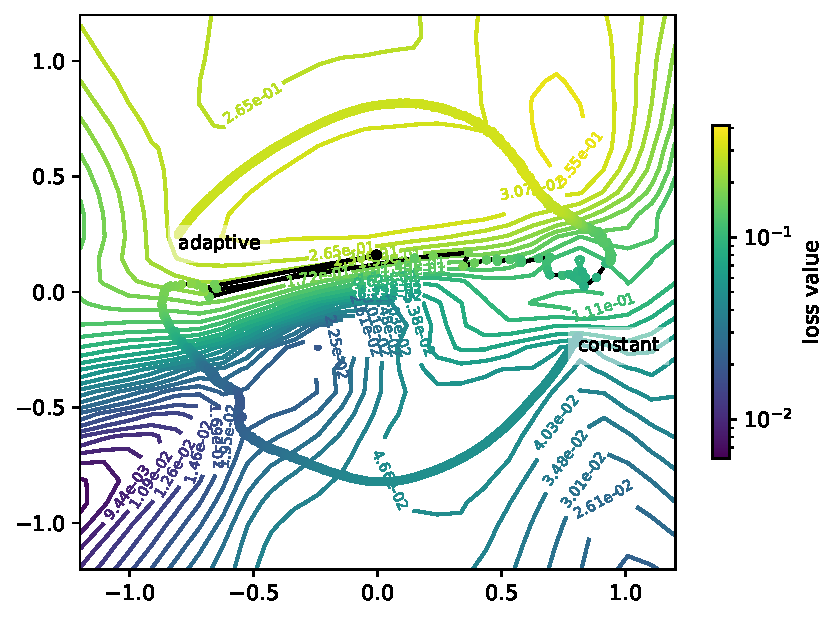
\includegraphics[width=\textwidth]{figures/round3/NTK/map_ic_train_loss_loss.pdf}
                \caption{initial condition loss ($\lic$)}
            \end{subfigure}
            % \hfill
            % \begin{subfigure}[b]{0.45\textwidth}
            %     \centering
            %     \includegraphics[width=\textwidth]{figures/round3/NTK/map_u_train_loss_loss - Copy.pdf}
            %     \caption{test loss ($\ltest$)}
            % \end{subfigure}
            
            \caption{A comparison of the two optimization approaches studied by \cite{wang2020and} using \proposedautencoder{}. This visualization verifies the authors' claims and shows that an NTK-based adaptive approach emphasizes on a better optimization of the boundary condition loss and reaches flatter minima across all losses.}
            \label{fig:PINNsNTK}
        \end{figure*}







           \subsubsection{Using \proposedautencoder{} To Study PINNs' Failure Modes.} \label{se:mahoney}

           Inspired by \cite{krishnapriyan2021characterizing}'s work on understanding the effect of the PDE's complexity and PINN's regularization 
          on the loss landscape and optimization outcome, we use \proposedautencoder{} to study PINN performance on the convection equation. Namely, we want to validate whether a higher $\beta$ parameter in a convection PDE or an increase in PINN regularization (i.e., an increase in the value of $\cres$) leads to a more complex loss landscape that is harder to optimize. As such, we run an experiment where we train PINNs with varying $\beta$ values, and then compare their loss landscapes using \proposedautencoder{}. A similar experiment on $\cres$ can be found in \cref{app:cres}. 
          %(see \cref{app:pdes}) 

          Looking at \cref{fig:FailsBeta}, it is easy to verify that an increase in $\beta$ renders the loss landscape more non-convex and harder to optimize. This agrees with the authors' findings. However, it is worth noting that the loss landscape visualizations presented in \cite{krishnapriyan2021characterizing}  used linear methods. When \cref{fig:FailsBeta} is compared to its counterpart (i.e.,  Figure 3 in \cite{krishnapriyan2021characterizing}), it is evident that their loss landscape visualizations are
          %, for the most part, 
          less intuitive and hard to visually interpret without the authors' commentary, indicating that our proposed method is more effective.
             


        \begin{figure*}[htb]
            \centering
            
            \begin{subfigure}[b]{0.3\textwidth}
                \centering
                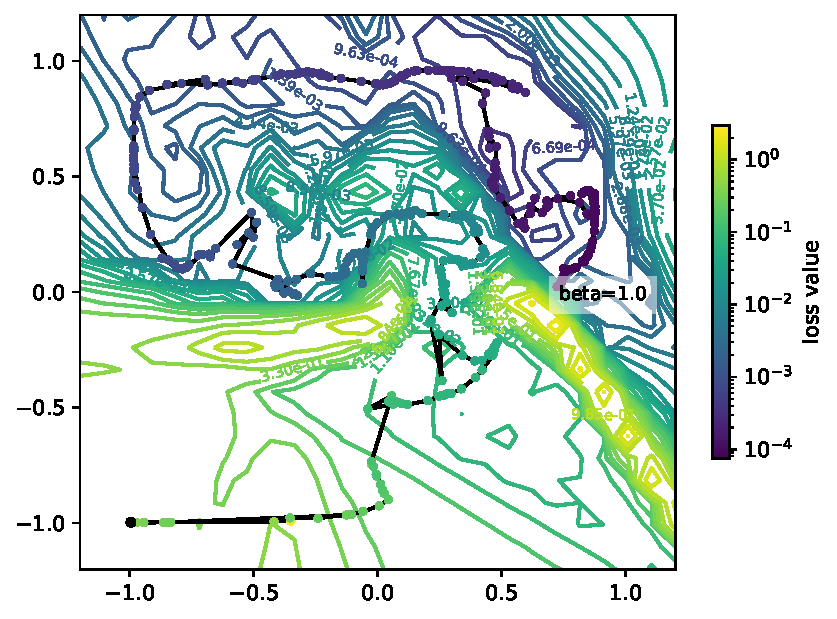
\includegraphics[width=\textwidth]{figures/round3/Fails/beta_/b1.pdf}
                \caption{$\beta=1$}
            \end{subfigure}
            \hfill
            \begin{subfigure}[b]{0.3\textwidth}
                \centering
                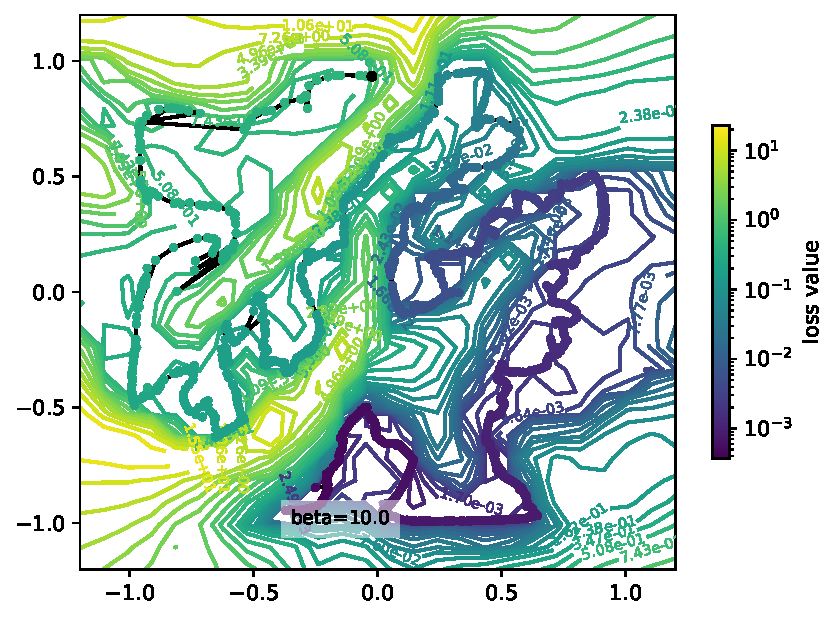
\includegraphics[width=\textwidth]{figures/round3/Fails/beta_/b10.pdf}
                \caption{$\beta=10$}
            \end{subfigure}
            % \begin{subfigure}[b]{0.45\textwidth}
            %     \centering
            %     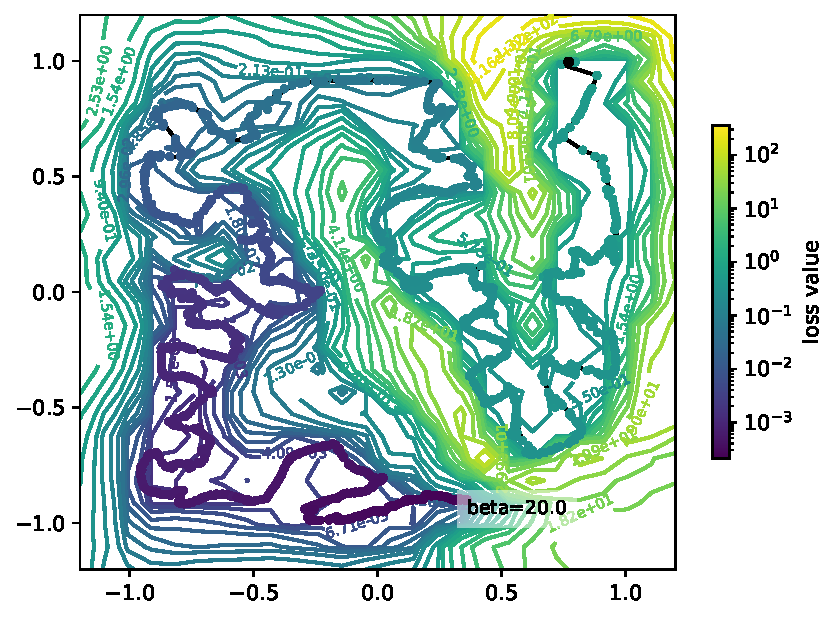
\includegraphics[width=\textwidth]{figures/round3/Fails/beta_/b20.pdf}
            %     \caption{$\beta=20$}
            % \end{subfigure}
            \hfill
            \begin{subfigure}[b]{0.3\textwidth}
                \centering
                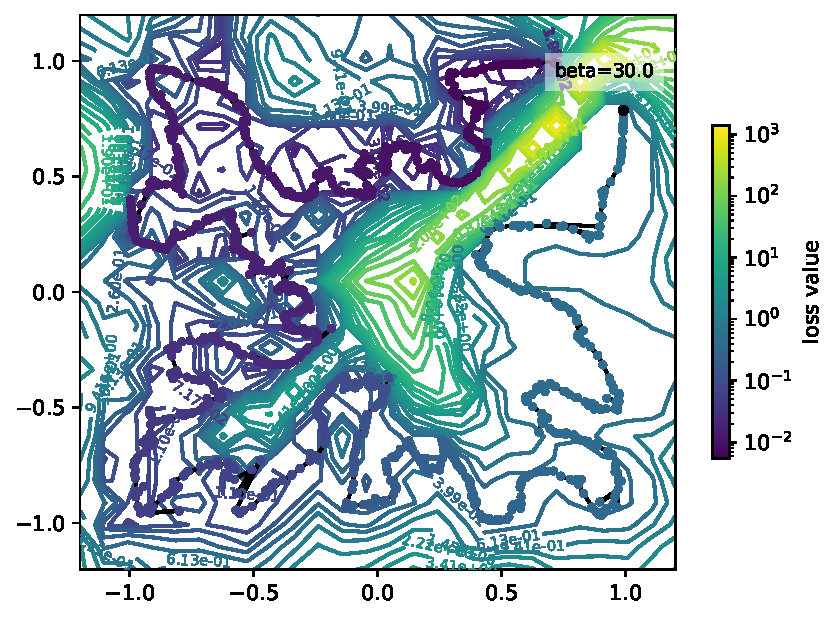
\includegraphics[width=\textwidth]{figures/round3/Fails/beta_/b30.pdf}
                \caption{$\beta=30$}
            \end{subfigure}
            
            \caption{A comparison of PINNs solving convection PDEs of varying $\beta$s. \proposedautencoder{} verifies the claim of \cite{krishnapriyan2021characterizing} that increasing $\beta$ causes $L_{total}$'s landscape to become more non-convex and difficult to optimize.}
            \label{fig:FailsBeta}
        \end{figure*}



           

           \subsubsection{Investigating Different Loss Balancing Techniques.} \label{sss:MTL}
           Balancing different loss terms in frameworks such as multi-task learning (MTL) or \SGML{} can be a daunting task \cite{wang2020and,doi:10.1137/20M1318043,elhamod2022cophy}. Thus, the ability to compare different loss balancing techniques is an important research effort. Generally, different loss balancing techniques are compared based on the final model's accuracy. 
           However, this metric 
           %omits much of the big picture, including a 
           does not provide a fundamental understanding of the optimization process 
           %for the different balancing methods. Additionally, it is desired to know 
           and whether a loss balancing algorithm is more suitable for one specific task than another. %struggles with one type of problems or architecture while being suitable for another. 
           %Finally, while some insight could be gained by looking at the loss per epoch plots, such a plot only shows the evolution of a single model instance, without necessarily describing the loss landscape more generally.

           % Expanding on the previous experiment to investigate the suitability of an \SGML{} framework and comparing it to other baselines, 
           Here, we consider six different loss balancing methods that are commonly used in the literature; namely Equal Weights (\ew{}), Constant Weights (\cw{}), Dynamic Weight Averaging (\dwa{}), Learning Rate Annealing \cite{doi:10.1137/20M1318043} (\lranneal{}), Gradient Normalization \cite{pmlr-v80-chen18a} (\gradnorm{}), and Random Loss Weighting \cite{lin2022reasonable}  (\rlw{}). 
           %PINNs are used to compare performance. 
           \cref{app:lossbalancing} gives a detailed account of these algorithms.
           %Since these methods typically differ in the criteria used to balance the loss terms, their optimization paths and the properties of their final models can vary widely. 
           %While three of these methods are selected from multi-task learning (MTL) literature, we also include a loss balancing algorithm that is more specific to PINNs. Namely, the Learning Rate Annealing method \cite{doi:10.1137/20M1318043}.
           % In multi-task learning, an algorithm is devised such that the coefficient of each loss is adaptively updated each epoch based on a certain criterion, such as the gradient of the losses. 
           % Additionally, I consider a loss balancing algorithm that is more specific to PINNs. Namely, the Learning Rate Annealing method \cite{doi:10.1137/20M1318043}. 
           % Finally, I also include two other naive baseline methods that do not involve dynamic coefficient updates. 
           

            %     \begin{table*}[htb]
            % \small
            % \centering
            % \resizebox{\textwidth}{!}{\begin{tabular}{|p{0.17\textwidth}|p{0.17\textwidth}|p{0.6\textwidth}|}
            % \hline
            % \textbf{Method} & \textbf{Abbreviation}  & \textbf{Brief description} \\
            % \hline
            % Equal Weights & \ew{} & All loss terms have a coefficient of $1.0$.\\
            % \hdashline
            % Constant Weights & \cw{} & Different constants are used to balance the loss terms. In the context of this section, the following values where used based on some hyper-parameter tuning: $\cres=1.0, \cic = \cbc=100.0$.\\
            % \hdashline
            % Dynamic Weight Averaging & \dwa{} & The weight of each task's loss is adjusted based on the relative improvement of that task's performance compared to the performance of the other tasks.\\
            % \hdashline
            % Learning Rate Annealing \cite{doi:10.1137/20M1318043} & \lranneal{} & Gradient statistics are utilized during model training to balance the interplay between the losses.\\
            % \hdashline
            % Gradient Normalization \cite{pmlr-v80-chen18a}& \gradnorm{} & Normalizes the gradients across tasks so that they have similar scales, encouraging the model to focus on the tasks with the most informative gradients. \\
            % \hdashline
            % Random Loss Weighting \cite{lin2022reasonable}& \rlw{} & The weight of each task is randomly updated each epoch.\\

            % \hline
            % \end{tabular}}

            
           To compare these algorithms, starting from the same model initialization, we train multiple PINNs with the listed algorithms to solve the Convection problem with $\beta=10$. %Each PINN uses a different loss balancing algorithm listed. 

        % Starting from the same initial model, I train six different instances of the model using the different loss balancing methods. 
        %Then, I plot the trajectories of these models on the same loss surface to give the full picture. In addition to the aforementioned loss terms involved in model optimization, I also plot the test mean-squared-error loss on unseen data-points. 
        In \cref{fig:dwa}, we inspect the landscapes of two loss terms: $\lres$ and $\ltest$. 
        %For each loss term, two loss landscape visualizations are produced using \proposedautencoder{} and PCA. 
        %Fig. \ref{fig:\dwa} shows the results for all losses.
        % Inspecting \cref{fig:\dwa}, we can make the following observations:
        % \begin{enumerate}
        % \item \textbf{\proposedautencoder{} detects model convergence more clearly:} Looking at \cref{subfig:testAE}, it is easy to see, 
        Using \proposedautencoder{}, 
        %we can see that all loss balancing methods, except for \lranneal{}, converge to some minima. Moreover, 
        the different trajectories and minima can be easily found and compared. In particular, it is clear that while \gradnorm{} and \ew{} take slightly different trajectories, they converge to the same minima. On the other hand, \dwa{} converges to the same basin as \gradnorm{} and \ew{} w.r.t $\lres$, but not the same minima.  
        %This analysis is possible thanks to the unique non-linear manifold \proposedautencoder{} learns, which allows for different scaling factors at different parts of the grid.
        Additionally, looking at \cref{subfig:testAE}, it is clear that \lranneal{}'s trajectory is nowhere near a minima w.r.t $\ltest$. This is surprising since \lranneal{} has shown success at solving the Helmholtz equation and the Klein Gordon equation as demonstrated in \cite{doi:10.1137/20M1318043}, implying that not all PINN tasks benefit from this method. %goes against the assumption that such a loss balancing method specifically designed for PINNs should perform better than the other generic methods. Thus, while \lranneal{} shows great success for solving the Helmholtz equation and the Klein Gordon equation as demonstrated in \cite{doi:10.1137/20M1318043}, it seems to fail at achieving good optimization for the Convection problem. Thanks to \proposedautencoder{}, it is easy to make this conclusion visually.
        The valuable insight that was visually, easily, and intuitively inferred from \proposedautencoder{} in \cref{fig:dwa} would not have been possible with a baseline method such as PCA due to its linear scale and planar manifold. \cref{app:MTLPCA} shows the equivalent results using PCA to verify this claim. 
        
      
        % It is also worth noting that while \proposedautencoder{}'s manifold does exhibit some fitting error in \cref{fig:dwa}, as evident from the difference in color between trajectory models and their corresponding grid background colors, it still fits the trajectories significantly better than that of PCAs. 
        % \cref{tab:quant_losslandscape2} demonstrates that quantitatively.

        % \begin{table}
        % \centering
        % \resizebox{\textwidth}{!}{\begin{tabular}{|c|c|c|}
        % \hline
        % \textbf{Method} & \textbf{Average absolute loss error} & \textbf{Average projection error in the parameter space} \\
        % \hline
        % \proposedautencoder{} & 0.147 & 1.583 \\
        % \hline
        % PCA & 0.923 & 12.801 \\
        % \hline
        % \end{tabular}}
        % \caption{A quantitative comparison of PCA and \proposedautencoder{} by calculating $\ltest$ errors between the trajectory and the grid in terms of loss values and distances in the parameter space.}
        % \label{tab:quant_losslandscape2}
        % \end{table}

            




         
            \section{Conclusions and Future Work} \label{se:conclusion}
                In this paper, we have shown that our proposed auto-encoder-based method, \proposedautencoder{}, is capable of learning non-linear manifolds in the input model parameter space and mapping such manifolds onto a 2-D grid for loss landscape visualization. Additionally, we have demonstrated that \proposedautencoder{} surpasses many other linear and non-linear landscape visualization approaches in terms of representation accuracy and malleability to learning manifolds with user-defined properties. Finally, we used two applications, \cophy{} \cite{elhamod2022cophy} and PINNs \cite{raissi2017physics1}, to derive insightful findings, including the importance of certain hyper-parameters for neural network training and the efficacy of different deep learning frameworks such as Multi-Task Learning (MTL) and Knowledge-Guided Machine Learning (\SGML). 
                % While the two application we chose in this paper allowed us to widely explore \proposedautencoder{}'s potency, 
                % much is left for 
                Future work could explore the full potential of \proposedautencoder{} by using it to study other deep learning phenomena, such as the relationship between landscape sharpness and generalizability \cite{pmlr-v137-huang20a}.
                
                One of \proposedautencoder{}'s limitations is the lack of scalability for large input parameter spaces. For example, the PINNs studied in this paper have an input dimensionality of the order of $10,000$ parameters, which is relatively small. In contrast, computer vision applications generally use much larger models (e.g., a VQ-GAN \cite{esser2021taming} has approximately $88$ million parameters).
                %in a . For example, a ResNet-18 \cite{resnet} has $11.2$ million parameters, and a VQ-GAN \cite{esser2021taming} can have as much as $88$ million parameters. 
                Such a large input space would be prohibitively difficult for \proposedautencoder{} to encode directly. A future research direction could investigate appropriate ways to encode and visualize such large models effectively. 
                %the use of certain techniques, such as network pruning \cite{NEURIPS2021_1cc8a8ea}, to reduce the dimensionality of the input parameter space so it could be encoded by \proposedautencoder{}.

                    
        \begin{figure}[H]
            \centering
              % \vspace{-2.5cm}
            % \begin{subfigure}[b]{0.4\textwidth}
            %     \includegraphics[width=\textwidth]{figures/MTL_new/directions.h5_proj_cos_bc_Convection.h5_Convection_bc_loss_2-Dcontour_proj.pdf}
            %     \caption{$\lbc$ - PCA}
            %   \end{subfigure}
            %   \hfill
            %   \begin{subfigure}[b]{0.4\textwidth}
            %     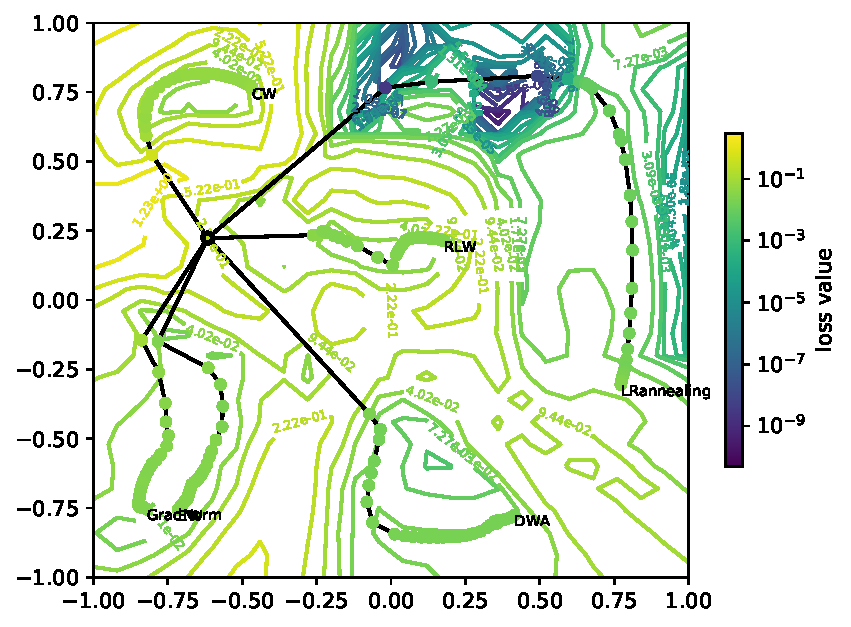
\includegraphics[width=\textwidth]{figures/MTL_new/map_bc_train_loss_loss.pdf}
            %     \caption{$\lbc$ - \proposedautencoder{}}
            %   \end{subfigure}
            % \vspace{1cm}
         

            %   \begin{subfigure}[b]{0.4\textwidth}
            %     \includegraphics[width=\textwidth]{figures/MTL_new/directions.h5_proj_cos_ic_Convection.h5_Convection_ic_loss_2-Dcontour_proj.pdf}
            %     \caption{$\lic$ - PCA}
            %   \end{subfigure}
            %   \hfill
            % \begin{subfigure}[b]{0.4\textwidth}
            %     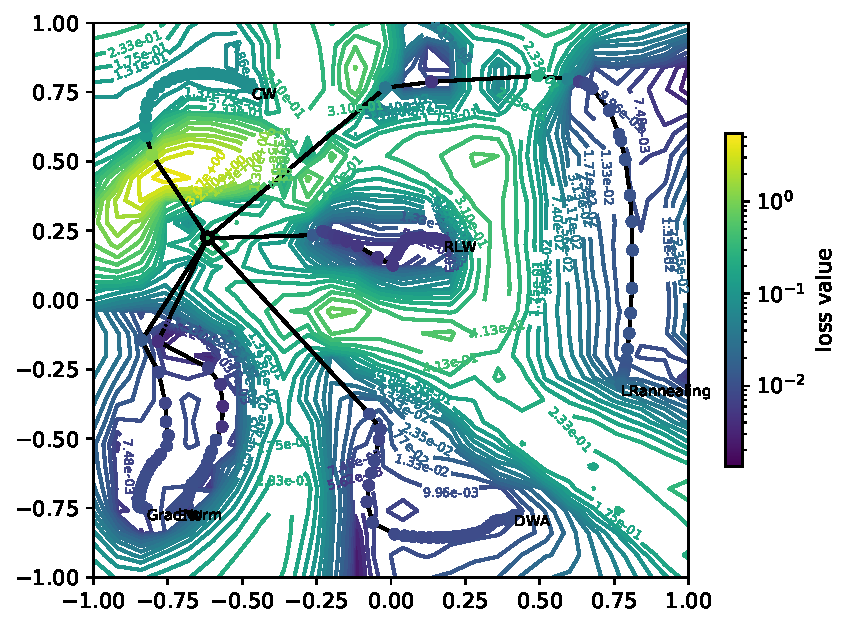
\includegraphics[width=\textwidth]{figures/MTL_new/map_ic_train_loss_loss.pdf}
            %     \caption{$\lic$ - \proposedautencoder{}}
            %     % \label{fig:subfig1}
            %   \end{subfigure}

                    % \vspace{1cm}
         

              \begin{subfigure}[b]{0.3\textwidth}
                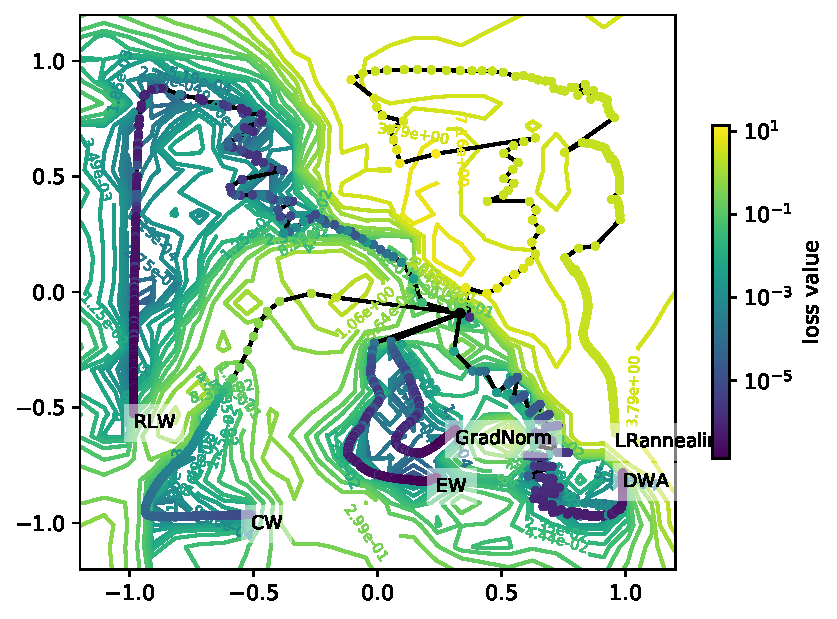
\includegraphics[width=\textwidth]{figures/round3/MTL2/map_residual_train_loss_loss.pdf}
                \caption{$\lres$}
                \label{subfig:residualAE}
                % \label{\proposedautencoder{}}
              \end{subfigure}
                % \hfill
              \begin{subfigure}[b]{0.3\textwidth}
                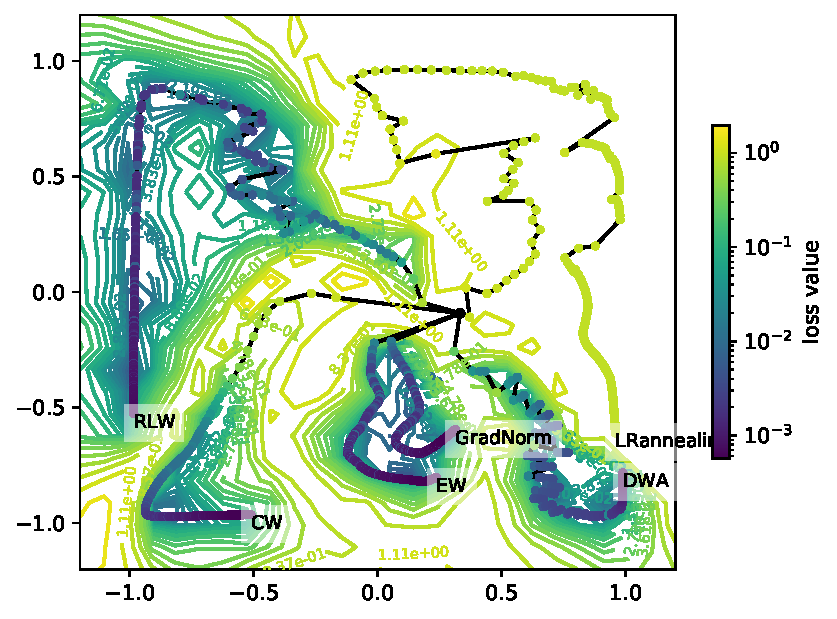
\includegraphics[width=\textwidth]{figures/round3/MTL2/map_test_mse_train_loss_loss.pdf}
                \caption{$\ltest$}
                            \label{subfig:testAE}
                % \label{\proposedautencoder{}}
              \end{subfigure}

              \caption{\proposedautencoder{}'s loss landscapes of PINN models with different loss balancing methods intuitively and visually provide valuable insights that would otherwise be hard to extract.}
              \label{fig:dwa}
            \end{figure}


% \clearpage
% \bibliographystyle{ACM-Reference-Format}

% \newpage

\bibliography{sample-base}
            
\clearpage

\appendix

      

    \section{Hyper-parameter Selection and Additional Implementation Details} \label{app:hyper}
            %%%%%
            To guarantee that an input model $m \in \manifold$ is encoded into $z \in [-1, +1]\times [-1, +1]$, a \textit{tanh} activation function is appended to the output of the encoder $\encoderlandscape$. Also, $m$ is normalized for an easier training of $\proposedautencodermodel$.

            With regards to location anchoring constraints $\lanch$, we here define the three different examples mentioned in \cref{p:anchoring} more rigorously: %\label{se:constaints}}:

            \begin{itemize}[itemsep=0em]
            \item \textit{Polar pinning (${\lanch}_1$) }: This can be formally defined by setting $\trajectorymodels^\prime = \{ m_{0}, m_{\left| \trajectorymodels \right|} \}$ (i.e., the set that contains the first and last models in the trajectory), and $\mathcal{A} = \{ (-r, -r), (r, r)\}$, with an $r=0.8$.
            \item \textit{Center pinning (${\lanch}_2$) }: It is formally defined with $\trajectorymodels^\prime = \{ m_{\left| \trajectorymodels \right|} \}$ and $\mathcal{A} = \{(0, 0)\}$.
            \item \textit{Circle pinning (${\lanch}_3$) }: It is formally defined with $\trajectorymodels^\prime = \{ m_{\left| \trajectorymodels \right|} \}$ and $\mathcal{A} = \{(r \cdot \text{sin}(\frac{2 \pi k}{n}) , r \cdot \text{cos}(\frac{2 \pi k}{n}))\ \text{where } k \in \{0, 1, ...,  n-1\}  \}$
            \end{itemize}

                        % \subsubsection{Trajectory spacing constraints:} \label{p:trajscaling}


            It is worth mentioning that we use another constraint, $\ltraj$, in some of our experiment to help space the trajectory models equally so that they are spread out across the grid. The loss term for this constraint penalizes for the differences in step sizes in the latent grid space between consecutive trajectory models.
            
            % It is also worth mentioning that another constraint that we use in our experiments is spacing the trajectory models' projections equally such that all optimization steps have the same resolution. For that, we construct a trajectory spacing constraint, $\ltraj$, such that: 
            
            % \begin{equation}
            %    \ltraj = \text{MSE}_{m_{i} \in \trajectorymodels} \left[ \left(\encoderlandscape(m_{i}) - \encoderlandscape(m_{i+1})\right)^2 , D^2 \right]
            % \end{equation}
            
            % where $D$ is a hyper-parameter that defines the appropriate distance between consecutive models in the grid space. In this work, We set $D = \frac{2 \pi r}{\left| \trajectorymodels \right|}$ where $r=0.8$ to maximize the utilized grid space. 
            % %This $D$ is the ideal distance between consecutive models that could fit the trajectory on a circle of radius $r$. However, $D$ can be set manually as desired for a shorter or a longer trajectory in the visualization.





            \cref{tbl:hyper} shows the hyper-parameters used to train \proposedautencoder{} for both \cophy{} and PINNs. %It is also worth noting that 

            \begin{table*}[htb]
            \begin{tabular}{|p{3cm}|l|l|l|l|l|}
            \hline
                           & encoder hidden layer sizes & batch size & epochs & lr   & notes                                                                                                                                   \\ \hline
            \cophy{}. \cref{ss:cophy_landscape2}         & $3141, 270, 23$               & $32$         & $40,000$  & $10^{-4}$ &                                                                                                                                         \\ \hdashline
            PINNs - "Investigating Different Loss Balancing Techniques". \cref{sss:MTL}  & $991, 125, 15$                 & $32$         & $600,000$ & $5 \times 10^{-4}$ & $\crec{} = 10^4$                                                                                                      \\ \hdashline
            PINNs - "Using \proposedautencoder{} To Study PINNs' Training Pathologies". \cref{ss:NTK}  & $1000, 500, 100$              & $32$         & $100,000$  & $10^{-5}$ & $\canch{}_3 = 10^4$                                              \\ \hdashline
            PINNs - "Using \proposedautencoder{} To Study PINNs' Failure Modes". \cref{se:mahoney} & $991, 125, 15$                 & $32$         & $600,000$ & $5 \times 10^{-4}$ & $\ctraj{} = 1$                                                                                                \\ \hdashline
            PINNs - "Demonstrating \proposedautencoder{}'s Flexibility With Different Constraints".  \cref{ss:constraints}  & $991, 125, 15$                 & $32$         & $80,000$  & $10^{-4}$ & \begin{tabular}[c]{l} $\canch{}_1 = 10^2$ \\ \\ $\canch{}_2 = 10^2$, $\cgrid{} = 1$ \end{tabular} \\ \hline
            \end{tabular} %\\ \\ $\canch{}_1 = 10^4$, $\ctraj{} = 10^4$

            \caption{A table of the hyper-parameter values used to train \proposedautencoder{} for each experiment.}
            \label{tbl:hyper}
            \end{table*}

            Finally, the experiments in this paper were run on Nvidia DGX A100 GPUs. Each experiment needed a single GPU and 8 CPU cores.

  \section{On the ``Correctness” of Loss Landscape Visualization Methods} \label{app:correctness}
            
           Loss landscape visualization is a subjective tool that provides a qualitative and holistic description of the landscape, rather than a quantitative one. As such, the notion of ``correctness" is not the best vantage point from which this tool can be appreciated. One analogy that clarifies this point is map projections. Earth map projections represent the 3-D Earth surface on a 2-D plane. Different projection methods have different advantages and limitations; each method makes certain features or characteristics of the Earth surface more or less prominent. Thus, there are many valid projections, each useful for different purposes. One popular method is the Mercator projection \cite{snyder1997flattening}, which is useful for navigation because it preserves angles and directions. However, it distorts the size and shape of objects near the poles. Another method is the Robinson projection \cite{snyder1990robinson}, which balances distortions of size and shape, making it a good all-purpose projection. 
           %However, it still distorts the sizes and shapes of landmasses, especially those near the poles. 
           A third method is the Winkel tripel projection \cite{snyder1997flattening} which 
           %compromises on the distortions of size and shape and 
           accurately shows the relative sizes and shapes of landmasses, but still distorts the shapes of some landmasses and oceans. 
           
           Similarly, a non-linear loss landscape visualization method will produce a non-linear manifold that gets distorted when visualized on a 2-D planar grid. . Thus, while the user should be aware of these distortions and understand the visualization accordingly, the method is still valid and useful for understanding the properties of the loss surface. And while there are infinitely many manifolds that could contain a set of points in the parameter space (i.e., models), it is important to select the manifold(s) that exhibits the desired user-defined criteria, such as the scaling factors at different parts of the manifold.





    \section{A Brief Description of \cophy{}} \label{app:cophy}


\cophy{} \cite{elhamod2022cophy}, short for Competing Physics Physics-Guided Neural Networks, is a model uniquely tailored to solve eigenvalue problems, which are prevalent in scientific domains such as quantum mechanics and electromagnetic propagation. In addition to the data-drive $\text{Train-Loss}$, two physics-guided (PG) loss terms are used: \text{\nsloss{}} and \text{\eloss{}}.\text{\nsloss{}} is designed to enforce the eigen-equation, and its minimization can lead to multiple solutions that satisfy the physical constraints of the problem. However, these multiple solutions may correspond to different energy levels. Generally, only one solution is desired. This is where S-Loss comes into play. \text{\eloss{}} guides the network towards the specific energy level of interest by minimizing the difference between the predicted and target eigenvalues
% , effectively narrowing down the correct solution from the multiple possibilities allowed by C-Loss.

The overall learning objective of \cophy{} is:
\begin{equation}
    E(t) = \text{Train-Loss} + \lambda_C(t) ~ \text{\nsloss{}} + \lambda_S(t)  ~\text{\eloss{}}
\end{equation}


The methodology of \cophy{} involves adaptively tuning the coefficients of these loss functions by annealing \( \lambda_S \) so as to steer the model towards the correct energy level in the initial stages of training. Conversely, \( \lambda_C \) is cold started, allowing the physical constraints to be gradually enforced and ensuring that the solution adheres to the underlying physics.

Using two applications – predicting the ground-state wave function of an Ising chain model in quantum mechanics, and modeling electromagnetic wave propagation in periodically stratified layer stacks – the authors demonstrate the effectiveness and extrapolative power of \cophy
%\cophy{} demonstrated its efficacy. By leveraging the complementary nature of S-Loss and C-Loss, the framework was able to navigate the complex landscape of eigenvalue problems, pinpointing solutions that are both physically consistent and aligned with the specific energy level of interest. This synergy between the two loss functions, coupled with the framework's computational efficiency, positions CoPhy-PGNN as a promising approach for large-scale physical systems, offering advantages over traditional numerical methods.



     
    
    \section{Loss Landscapes Error Plots For \cophy{}} \label{app:errors_cophy}

    Following up on \cref{fig:PCAvsAE}, and to visually illustrate the results of \cref{tab:quant_losslandscape}, \cref{fig:PCAvsAE2,fig:UMAPKernelPCA_app} show the absolute loss error (i.e., the error between model loss and the loss at its projection on the learned manifold) in the first row, 
    %for the same \cophy{} training trajectory and visualization methods. It is clear that PCA results in higher errors in the loss values compared to \proposedautencoder{}. A similar and consistent observation can be made by looking at the second row of \cref{fig:PCAvsAE2} where the points are color-coded as 
    and the distance between the models and the manifold \underline{in the parameter space} in the second row. In both cases, the ``hot" model colors of baseline methods, compared to \proposedautencoder{}, indicate that the resulting manifold or plane is not a good fit for the trajectory.%distances between the models and the manifold are large. 
    %This is in contrast to the cool colors in \proposedautencoder{}'s view \cref{fig:PCAvsAE2_distances}), implying that the manifold fits the trajectory models well.

     

        \begin{figure}[htbp]
              \centering
              \begin{subfigure}[b]{0.3\textwidth}
                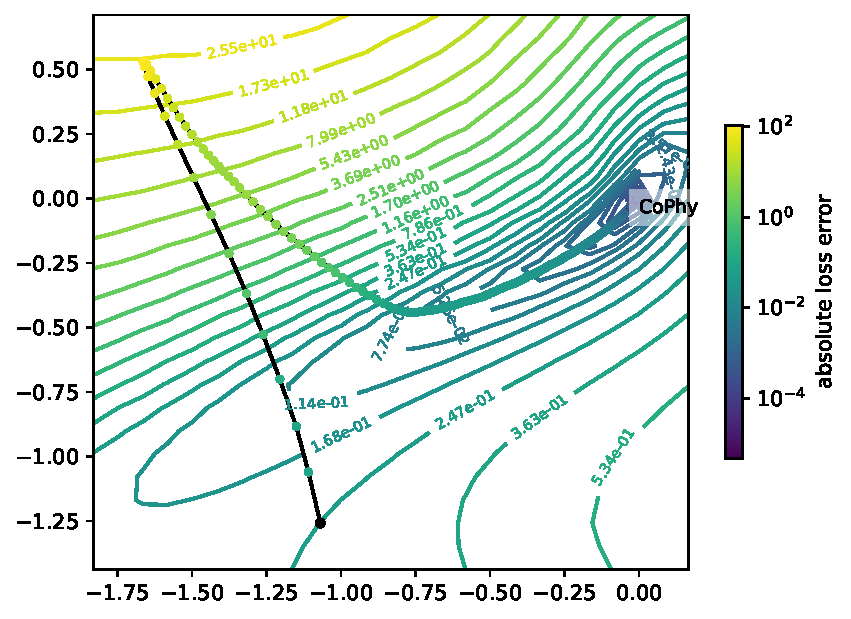
\includegraphics[width=\textwidth]{figures/round3/Cophy_PCA/directions.h5_proj_cos_phy_total.h5_total_phy_abs_error_2dcontour_proj.pdf}
                \caption{PCA}
                \label{fig:PCAvsAE2_PCAlosses}
              \end{subfigure}
              % \hfill
              \begin{subfigure}[b]{0.3\textwidth}
                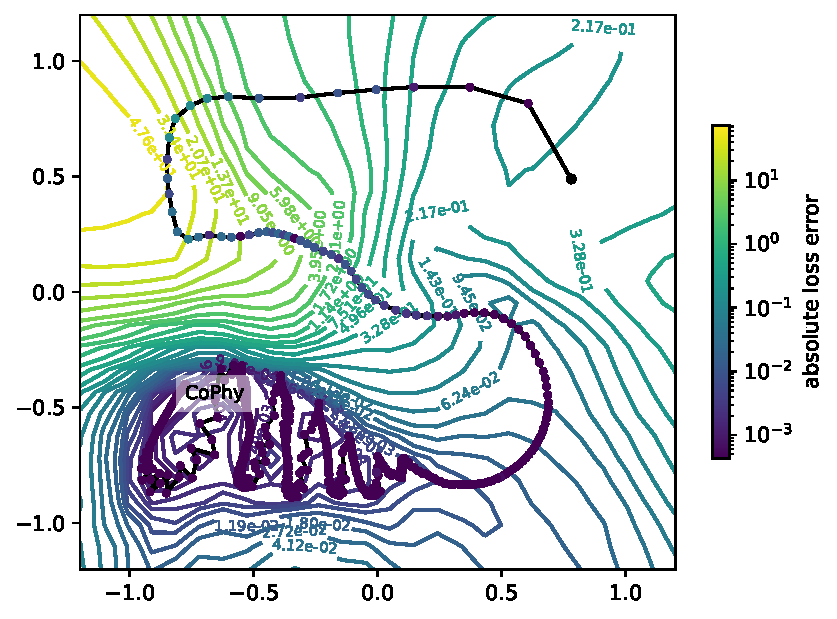
\includegraphics[width=\textwidth]{figures/round3/Cophy_NV/map_phy_total_abs_error.pdf}
                \caption{\proposedautencoder{}}
                \label{fig:PCAvsAE2_losses}
              \end{subfigure}
                    % \vspace{1cm}
              \begin{subfigure}[b]{0.3\textwidth}
                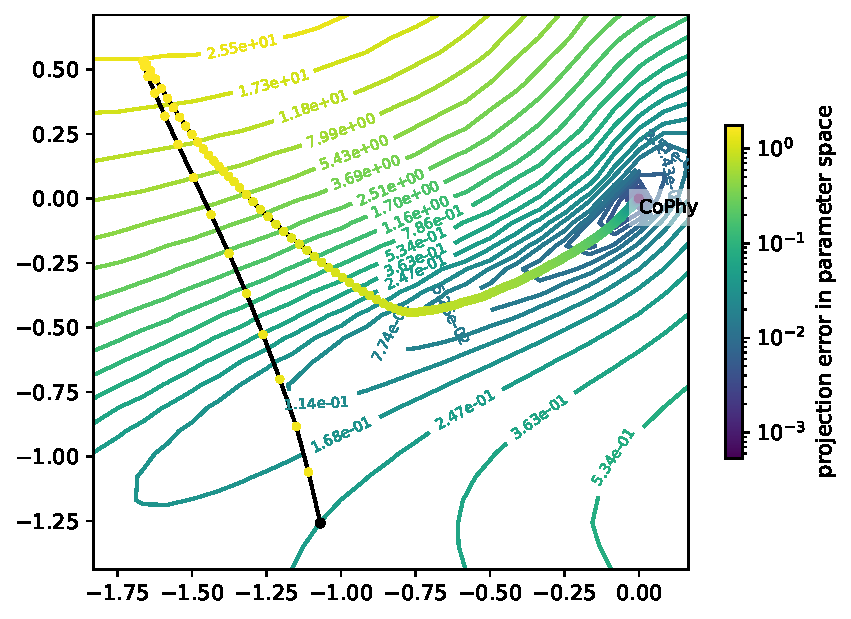
\includegraphics[width=\textwidth]{figures/round3/Cophy_PCA/directions.h5_proj_cos_phy_total.h5_total_phy_dists_param_space_2dcontour_proj.pdf}
                \caption{PCA}
                \label{fig:PCAvsAE2_PCAdistances}
              \end{subfigure}
              % \hfill
              \begin{subfigure}[b]{0.3\textwidth}
                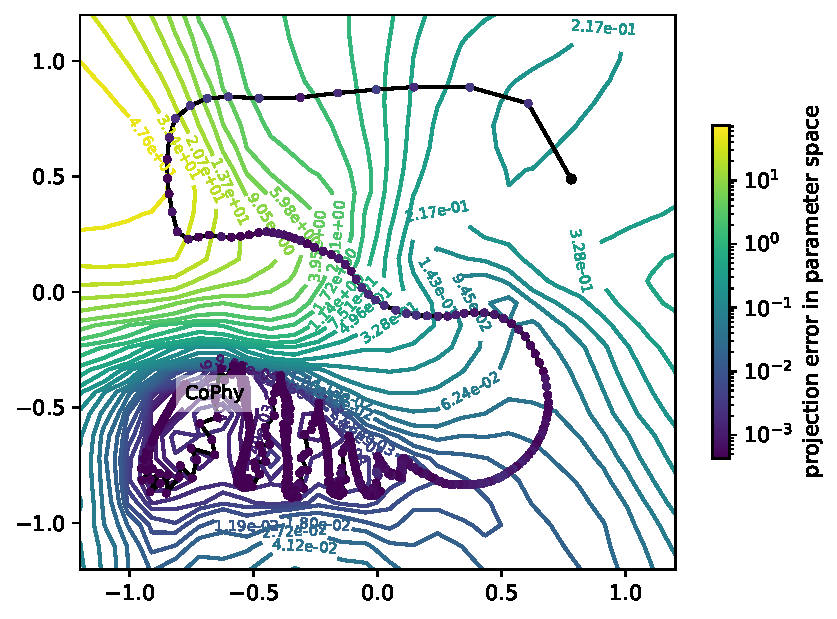
\includegraphics[width=\textwidth]{figures/round3/Cophy_NV/map_phy_total_dists_param_space.pdf}
                \caption{\proposedautencoder{}}
                \label{fig:PCAvsAE2_distances}
              \end{subfigure}

              \caption{A comparison of PCA and \proposedautencoder{} in terms of the error in \cophy{}'s total physics loss values (top two sub-figures) as well as projection errors (bottom two sub-figures). Note that the contour colors still refer to the loss values, similar to \cref{fig:PCAvsAE}. \proposedautencoder{} has lower error levels than PCA.}
              \label{fig:PCAvsAE2}
            \end{figure}




        \begin{figure}
              \centering
              \begin{subfigure}[b]{0.3\textwidth}
                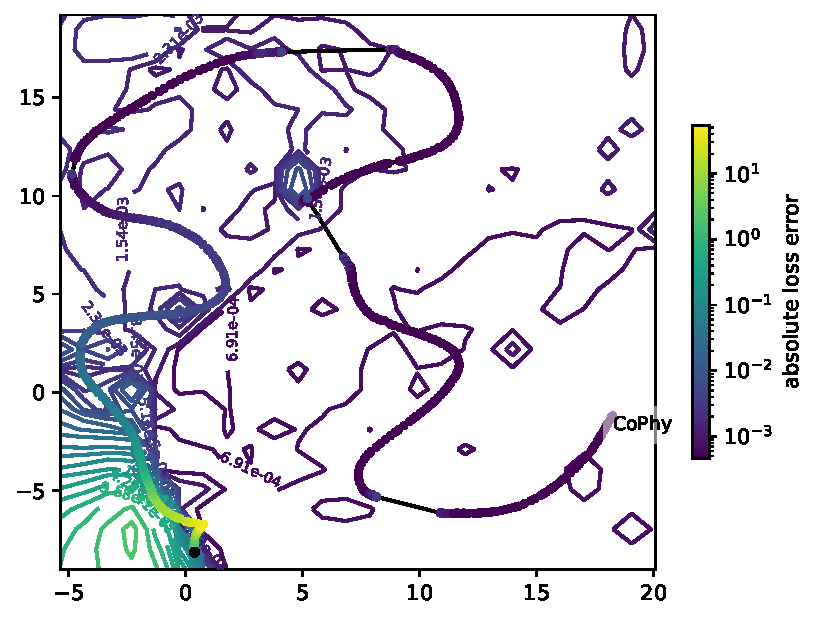
\includegraphics[width=\textwidth]{figures/round3/UMAP/map_phy_total_abs_error.pdf}
                % \caption{Caption for image 1}
                % \label{fig:subfig1}
                \caption{UMAP}
              \end{subfigure}
              % \hfill
              \begin{subfigure}[b]{0.3\textwidth}
                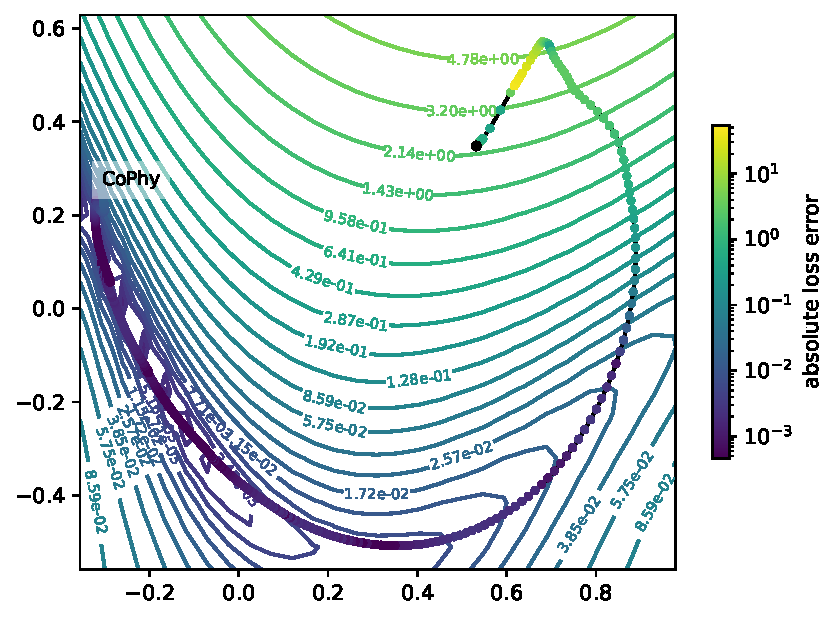
\includegraphics[width=\textwidth]{figures/round3/Kernel-PCA/map_phy_total_abs_error.pdf}
                \caption{Kernel-PCA}
              \end{subfigure}
                    % \vspace{1cm}
              \begin{subfigure}[b]{0.3\textwidth}
                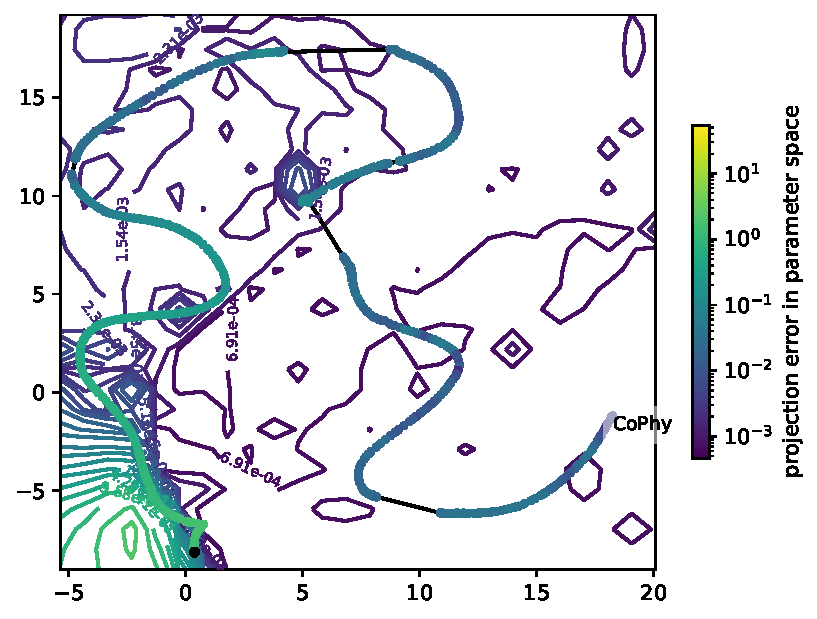
\includegraphics[width=\textwidth]{figures/round3/UMAP/map_phy_total_dists_param_space.pdf}
                \caption{UMAP}
                % \label{fig:subfig1}
              \end{subfigure}
              % \hfill
              \begin{subfigure}[b]{0.3\textwidth}
                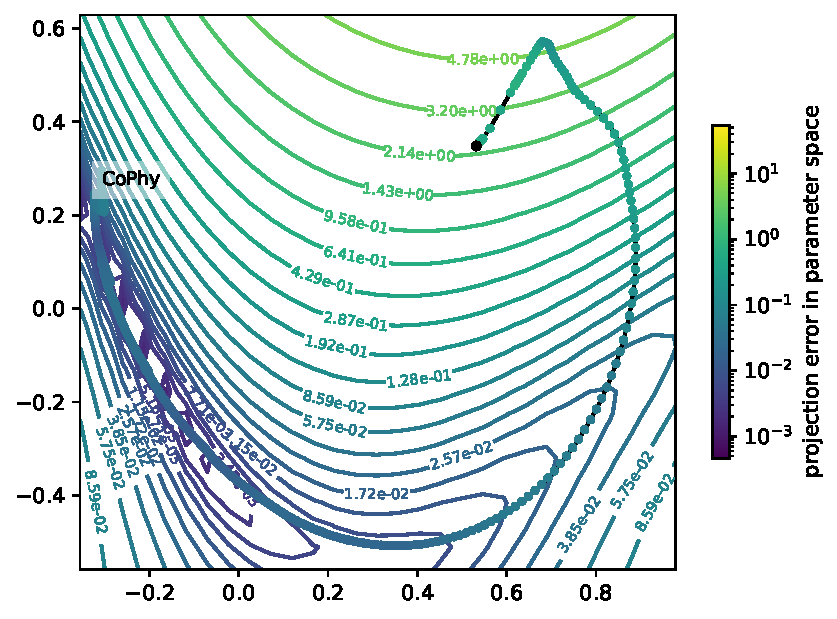
\includegraphics[width=\textwidth]{figures/round3/Kernel-PCA/map_phy_total_dists_param_space.pdf}
                \caption{Kernel-PCA}
                \label{fig:subfig2}
              \end{subfigure}

              \caption{A comparison of UMAP and Kernel-PCA in terms of the error in \cophy{}'s total physics loss errors (top row) and projection errors (bottom row). Compared to \cref{fig:PCAvsAE2}, neither UMAP nor Kernel-PCA look favorable against \proposedautencoder{}. Note that the contour colors still refer to the loss values, similar to \cref{fig:PCAvsAE}. %\cref{fig:UMAPKernelPCA}
              }
              \label{fig:UMAPKernelPCA_app}
            \end{figure}

   \section{Solving Partial Differential Equations with Physics-Informed Neural Networks (PINNs)} \label{app:pdes}

        Solving partial differential equations (PDEs) is a fundamental problem in many areas of science and engineering. Traditional numerical methods, such as finite element and finite difference methods, require a discretization of the domain and the PDEs, which can lead to high-dimensional and computationally expensive systems. Physics-informed neural networks (PINNs) \cite{raissi2017physics2, raissi2019physics, raissi2017physics1, GAO2021110079} have emerged as an alternative approach to solving PDEs, leveraging the representational power of neural networks and the structure of the underlying physics to learn a solution without discretization.

        PINNs have shown great promise in solving various types of PDEs, including elliptic, parabolic, and hyperbolic problems. The main idea behind PINNs is to parameterize the solution of a PDE with a neural network and enforce the governing equations as constraints in the training process. This is achieved by incorporating the PDEs as a loss function that is minimized during training, along with a data-driven loss term that incorporates observed data. 

        PINNs' optimization objective comes in a number of different forms. Generally, however, there are three main losses that are present. 
        The residual loss, $\lres$, is the most important term and ensures that the neural network satisfies the PDE at every point in the domain. It is calculated as the mean squared difference between the residual of the PDE and the output of the neural network at each point. $\lic$ ensures that the neural network satisfies the PDE at the initial condition. It is calculated as the mean squared difference between the output of the neural network at the initial time and the true initial condition. $\lbc$ ensures that the neural network satisfies the PDE at the boundary conditions. It is calculated as the mean squared difference between the output of the neural network at each boundary point and the true boundary condition. Together, these three loss terms provide a comprehensive approach to training PINNs to solve PDEs. By balancing these terms, the neural network can learn the underlying physics of the problem and provide accurate solutions.

        PINNs have been shown to be effective in solving a wide range of partial differential equations (PDEs). For example, in fluid mechanics, PINNs have been used to solve problems related to incompressible Navier-Stokes equations \cite{JIN2021109951}. Similarly, PINNs have also been used to solve the Schrödinger equation in quantum mechanics \cite{li2022mix}.

        This paper has targeted a certain type of PDEs called the ``convection equation" to illustrate the usefulness and superiority of the proposed model. The convection problem is a type of partial differential equation that arises in fluid mechanics and heat transfer. It models the transport of a quantity (such as mass, energy, or momentum) by a moving fluid, which can induce a net flow in the direction of the transport. The convection equation is:
        
        \begin{equation}
            f = u_t - \beta u_x
        \end{equation}

        where the parameter $\beta$ is the convection coefficient which represents the tendency of the substance to move with the fluid flow. 

        While PINNs have been useful at solving PDEs, the application of PINNs is not without challenges \cite{wang2020and,doi:10.1137/20M1318043}. In terms of the convection problem, one major challenge is the presence of the convection term $\beta$ in the governing equations, which is highly nonlinear and can result in optimization difficulties, especially for higher values. Another challenge is the presence of multiple scales in convection problems, which can lead to numerical instability and slow convergence. 


 
    \section{The Pathological Effect of Increasing Regularization in PINNs} \label{app:cres}

    Similar to \cref{fig:FailsBeta} where the pathological effect of increasing $\beta$ is displayed, \cref{fig:FailsL} shows the effect of increasing $\cres$. Clearly, increasing the regularization factor also leads to an increase in loss landscape complexity.  
    
        \begin{figure*}[hb]
            \centering
            
            \begin{subfigure}[b]{0.3\textwidth}
                \centering
                \includegraphics[width=\textwidth]{figures/round3/Fails/L_/L-6.pdf}
                \caption{$L=10^{-6}$}
            \end{subfigure}
            \hfill
            % \begin{subfigure}[b]{0.3\textwidth}
            %     \centering
            %     \includegraphics[width=\textwidth]{figures/round3/Fails/L_/L-5.pdf}
            %     \caption{$L=10^{-5}$}
            % \end{subfigure}
            \begin{subfigure}[b]{0.3\textwidth}
                \centering
                \includegraphics[width=\textwidth]{figures/round3/Fails/L_/L-3.pdf}
                \caption{$L=10^{-3}$}
            \end{subfigure}
            \hfill
            \begin{subfigure}[b]{0.3\textwidth}
                \centering
                \includegraphics[width=\textwidth]{figures/round3/Fails/L_/L-1.pdf}
                \caption{$L=10^{-1}$}
            \end{subfigure}
            
            \caption{A comparison of convection-PDE-solving PINNs with different degrees of soft regularization. \proposedautencoder{} verifies the authors' claim \cite{krishnapriyan2021characterizing} that increasing $\cres$ leads to an $L_{total}$'s landscape that is more non-convex and difficult to optimize.}
            \label{fig:FailsL}
        \end{figure*}
   
    






    \section{A PCA Loss Landscape Analysis of Loss Balancing Methods} \label{app:MTLPCA}
        %%%%%
         \cref{fig:dwaPCA} shows the PCA loss landscape for the same models in the loss balancing experiment outlined in \cref{sss:MTL} and visualized in \cref{fig:dwa}. As can be seen, PCA fails at delineating whether most models converge at all, converge to the same minima, converge to several minima in the same basin, or different basins altogether.

                                
        \begin{figure}[htb]
            \centering
              % \vspace{-2.5cm}
            % \begin{subfigure}[b]{0.4\textwidth}
            %     \includegraphics[width=\textwidth]{figures/MTL_new/directions.h5_proj_cos_bc_Convection.h5_Convection_bc_loss_2-Dcontour_proj.pdf}
            %     \caption{$\lbc$ - PCA}
            %   \end{subfigure}
            %   \hfill
            %   \begin{subfigure}[b]{0.4\textwidth}
            %     \includegraphics[width=\textwidth]{figures/MTL_new/map_bc_train_loss_loss.pdf}
            %     \caption{$\lbc$ - \proposedautencoder{}}
            %   \end{subfigure}
            % \vspace{1cm}
            %   \begin{subfigure}[b]{0.4\textwidth}
            %     \includegraphics[width=\textwidth]{figures/MTL_new/directions.h5_proj_cos_ic_Convection.h5_Convection_ic_loss_2-Dcontour_proj.pdf}
            %     \caption{$\lic$ - PCA}
            %   \end{subfigure}
            %   \hfill
            % \begin{subfigure}[b]{0.4\textwidth}
            %     \includegraphics[width=\textwidth]{figures/MTL_new/map_ic_train_loss_loss.pdf}
            %     \caption{$\lic$ - \proposedautencoder{}}
            %     % \label{fig:subfig1}
            %   \end{subfigure}
                    % \vspace{1cm}
              \begin{subfigure}[b]{0.3\textwidth}
                \includegraphics[width=\textwidth]{figures/round3/MTL_PCA/directions.h5_proj_cos_residual_Convection.h5_Convection_residual_loss_2dcontour_proj.pdf}
                % \caption{$\lres$ - PCA}
                % \label{fig:subfig1}
              \end{subfigure}
              % \hfill{}
                \begin{subfigure}[b]{0.3\textwidth}
                \includegraphics[width=\textwidth]{figures/round3/MTL_PCA/directions.h5_proj_cos_test_mse_Convection.h5_Convection_test_mse_loss_2dcontour_proj.pdf}
                % \caption{$\ltest$ - PCA}
                % \label{fig:testPCA}
              \end{subfigure}


              \caption{PCA's loss landscapes of multiple PINN models with different loss balancing methods. Clearly, it is hard to make useful or accurate inferences from this plot compared to the insights found through \cref{fig:dwa}. }
              \label{fig:dwaPCA}
            \end{figure}

    \section{Description of Different Loss Balancing Algorithms} \label{app:lossbalancing}

    \cref{tab:MTLmethods} expands on the different loss balancing algorithms that were used in \cref{sss:MTL} and shown in \cref{fig:dwa}.
    

                \begin{table*}[htb]
            \small
            \centering
            \resizebox{\textwidth}{!}{\begin{tabular}{|p{0.17\textwidth}|p{0.17\textwidth}|p{0.6\textwidth}|}
            \hline
            \textbf{Method} & \textbf{Abbreviation}  & \textbf{Brief description} \\
            \hline
            Equal Weights & \ew{} & All loss terms have a coefficient of $1.0$.\\
            \hdashline
            Constant Weights & \cw{} & Different constants are used to balance the loss terms. In the context of this section, the following values where used based on some hyper-parameter tuning: $\cres=1.0, \cic = \cbc=100.0$.\\
            \hdashline
            Dynamic Weight Averaging & \dwa{} & The weight of each task's loss is adjusted based on the relative improvement of that task's performance compared to the performance of the other tasks.\\
            \hdashline
            Learning Rate Annealing \cite{doi:10.1137/20M1318043} & \lranneal{} & Gradient statistics are utilized during model training to balance the interplay between the losses.\\
            \hdashline
            Gradient Normalization \cite{pmlr-v80-chen18a}& \gradnorm{} & Normalizes the gradients across tasks so that they have similar scales, encouraging the model to focus on the tasks with the most informative gradients. \\
            \hdashline
            Random Loss Weighting \cite{lin2022reasonable}& \rlw{} & The weight of each task is randomly updated each epoch.\\

            \hline
            \end{tabular}}
            
            \caption{A list of the loss balancing algorithms considered in \cref{sss:MTL}. More details on each algorithm can be found in \cite{liang2020simple}. }
            \label{tab:MTLmethods}
            \end{table*}
            
              %This is in contrast to PCA's landscape in \cref{fig:testPCA} where it is unclear whether several trajectories (e.g., \rlw{}, \gradnorm{}, and \dwa) converge at all because the grid does not show any minima where they terminate. Thus, \proposedautencoder{} is evidently more intuitive and useful for a qualitative assessment of these different methods.
        
        %\item 
        % \textbf{\proposedautencoder{} is more capable of distinguishing among different minima:} Looking at the residual loss (top row), it is unclear in the PCA plot (left) whether some of the loss balancing methods converge to the same minima, several minima in the same basin, or different basins altogether. This is due to the limited view and the unfavorable scale PCA's linear projection provides. In contrast, the loss landscape plotted using \proposedautencoder{} shows a much more holistic view of the loss balancing methods and how their trajectories compare. In particular, it clearly shows that while \gradnorm{} and \ew{} take slightly different trajectories, they converge to the same minima. Additionally, \proposedautencoder{} shows that \dwa converges to the same basin as \gradnorm{} and \ew{}, but not the same minima. This is in contrast to PCA's view where all three models are lumped together. This analysis would not be possible without the unique non-linear manifold \proposedautencoder{} learns, which allows for different scaling factors at different parts of the space.

        %\item It is clear that the loss landscape of this PINN is highly irregular and fraught with non-convexity and local minima. While PCA (left) shows some of this non-convexity, the picture \proposedautencoder{}  provides is much more detailed, especially when it comes to showing the details of the optimization process at its late stages.
        %\item 
        % \textbf{\proposedautencoder{} helps discover novel insights:} Looking at \cref{subfig:testAE}, 
        % %across the three optimization losses, it is clear that while the model achieves good optimization w.r.t $\lic$ 
        % it is clear that \lranneal{}'s trajectory is nowhere near a minima w.r.t $\ltest$. This goes against the initial expectation that such a loss balancing method specifically designed for PINNs should perform better than the other methods. Thus, while \lranneal{} shows great success for solving the Helmholtz equation and the Klein Gordon equation as demonstrated in \cite{doi:10.1137/20M1318043}, it seems to fail at achieving good optimization for the Convection problem. Thanks to \proposedautencoder{}, it is easy to make this conclusion visually.
        %In fact, the algorithm skips a local minima w.r.t $\lres$ due to the interplay with other losses. This interplay ends up placing \lranneal{} at a non-minima w.r.t to $\ltest$. This story is missing in the PCA column on the left. It is worth noting here that while \lranneal{} shows great success for solving the Helmholtz equation and the Klein Gordon equation \cite{wang2020understanding}, it seems to fail at achieving good optimization for the Convection problem. The landscape visualization tool helps shed some light on this limitation.
        %\item Looking at the landscapes in Figs. \ref{subfig:residualAE} and \ref{subfig:testAE}, it becomes obvious that the model that generalizes best (i.e., \dwa) need not have the lowest minim w.r.t $\lres$. This reinforces the result we saw in Section \ref{ss:cophy_landscape} where it was shown that the label-free model (i.e., \lfmodel) does not generalize well even though it achieves low values in terms of the physics losses.
        % \end{enumerate}




% \section{Preparing an Anonymous Submission}

% This document details the formatting requirements for anonymous submissions. The requirements are the same as for camera ready papers but with a few notable differences:

% \begin{itemize}
%     \item Anonymous submissions must not include the author names and affiliations. Write ``Anonymous Submission'' as the ``sole author'' and leave the affiliations empty.
%     \item The PDF document's metadata should be cleared with a metadata-cleaning tool before submitting it. This is to prevent leaked information from revealing your identity.
%     \item References must be anonymized whenever the reader can infer that they are to the authors' previous work.
%     \item AAAI's copyright notice should not be included as a footer in the first page.
%     \item Only the PDF version is required at this stage. No source versions will be requested, nor any copyright transfer form.
% \end{itemize}

% You can achieve all of the above by enabling the \texttt{submission} option when loading the \texttt{aaai24} package:

% \begin{quote}\begin{scriptsize}\begin{verbatim}
% \documentclass[letterpaper]{article}
% \usepackage[submission]{aaai24}
% \end{verbatim}\end{scriptsize}\end{quote}

% The remainder of this document are the original camera-
% ready instructions. Any contradiction of the above points
% ought to be ignored while preparing anonymous submis-
% sions.

% \section{Camera-Ready Guidelines}

% Congratulations on having a paper selected for inclusion in an AAAI Press proceedings or technical report! This document details the requirements necessary to get your accepted paper published using PDF\LaTeX{}. If you are using Microsoft Word, instructions are provided in a different document. AAAI Press does not support any other formatting software.

% The instructions herein are provided as a general guide for experienced \LaTeX{} users. If you do not know how to use \LaTeX{}, please obtain assistance locally. AAAI cannot provide you with support and the accompanying style files are \textbf{not} guaranteed to work. If the results you obtain are not in accordance with the specifications you received, you must correct your source file to achieve the correct result.

% These instructions are generic. Consequently, they do not include specific dates, page charges, and so forth. Please consult your specific written conference instructions for details regarding your submission. Please review the entire document for specific instructions that might apply to your particular situation. All authors must comply with the following:

% \begin{itemize}
% \item You must use the 2024 AAAI Press \LaTeX{} style file and the aaai24.bst bibliography style files, which are located in the 2024 AAAI Author Kit (aaai24.sty, aaai24.bst).
% \item You must complete, sign, and return by the deadline the AAAI copyright form (unless directed by AAAI Press to use the AAAI Distribution License instead).
% \item You must read and format your paper source and PDF according to the formatting instructions for authors.
% \item You must submit your electronic files and abstract using our electronic submission form \textbf{on time.}
% \item You must pay any required page or formatting charges to AAAI Press so that they are received by the deadline.
% \item You must check your paper before submitting it, ensuring that it compiles without error, and complies with the guidelines found in the AAAI Author Kit.
% \end{itemize}

% \section{Copyright}
% All papers submitted for publication by AAAI Press must be accompanied by a valid signed copyright form. They must also contain the AAAI copyright notice at the bottom of the first page of the paper. There are no exceptions to these requirements. If you fail to provide us with a signed copyright form or disable the copyright notice, we will be unable to publish your paper. There are \textbf{no exceptions} to this policy. You will find a PDF version of the AAAI copyright form in the AAAI AuthorKit. Please see the specific instructions for your conference for submission details.

% \section{Formatting Requirements in Brief}
% We need source and PDF files that can be used in a variety of ways and can be output on a variety of devices. The design and appearance of the paper is strictly governed by the aaai style file (aaai24.sty).
% \textbf{You must not make any changes to the aaai style file, nor use any commands, packages, style files, or macros within your own paper that alter that design, including, but not limited to spacing, floats, margins, fonts, font size, and appearance.} AAAI imposes requirements on your source and PDF files that must be followed. Most of these requirements are based on our efforts to standardize conference manuscript properties and layout. All papers submitted to AAAI for publication will be recompiled for standardization purposes. Consequently, every paper submission must comply with the following requirements:

% \begin{itemize}
% \item Your .tex file must compile in PDF\LaTeX{} --- (you may not include .ps or .eps figure files.)
% \item All fonts must be embedded in the PDF file --- including your figures.
% \item Modifications to the style file, whether directly or via commands in your document may not ever be made, most especially when made in an effort to avoid extra page charges or make your paper fit in a specific number of pages.
% \item No type 3 fonts may be used (even in illustrations).
% \item You may not alter the spacing above and below captions, figures, headings, and subheadings.
% \item You may not alter the font sizes of text elements, footnotes, heading elements, captions, or title information (for references and mathematics, please see the limited exceptions provided herein).
% \item You may not alter the line spacing of text.
% \item Your title must follow Title Case capitalization rules (not sentence case).
% \item \LaTeX{} documents must use the Times or Nimbus font package (you may not use Computer Modern for the text of your paper).
% \item No \LaTeX{} 209 documents may be used or submitted.
% \item Your source must not require use of fonts for non-Roman alphabets within the text itself. If your paper includes symbols in other languages (such as, but not limited to, Arabic, Chinese, Hebrew, Japanese, Thai, Russian and other Cyrillic languages), you must restrict their use to bit-mapped figures. Fonts that require non-English language support (CID and Identity-H) must be converted to outlines or 300 dpi bitmap or removed from the document (even if they are in a graphics file embedded in the document).
% \item Two-column format in AAAI style is required for all papers.
% \item The paper size for final submission must be US letter without exception.
% \item The source file must exactly match the PDF.
% \item The document margins may not be exceeded (no overfull boxes).
% \item The number of pages and the file size must be as specified for your event.
% \item No document may be password protected.
% \item Neither the PDFs nor the source may contain any embedded links or bookmarks (no hyperref or navigator packages).
% \item Your source and PDF must not have any page numbers, footers, or headers (no pagestyle commands).
% \item Your PDF must be compatible with Acrobat 5 or higher.
% \item Your \LaTeX{} source file (excluding references) must consist of a \textbf{single} file (use of the ``input" command is not allowed.
% \item Your graphics must be sized appropriately outside of \LaTeX{} (do not use the ``clip" or ``trim'' command) .
% \end{itemize}

% If you do not follow these requirements, your paper will be returned to you to correct the deficiencies.

% \section{What Files to Submit}
% You must submit the following items to ensure that your paper is published:
% \begin{itemize}
% \item A fully-compliant PDF file.
% \item Your \LaTeX{} source file submitted as a \textbf{single} .tex file (do not use the ``input" command to include sections of your paper --- every section must be in the single source file). (The only allowable exception is .bib file, which should be included separately).
% \item The bibliography (.bib) file(s).
% \item Your source must compile on our system, which includes only standard \LaTeX{} 2020 TeXLive support files.
% \item Only the graphics files used in compiling paper.
% \item The \LaTeX{}-generated files (e.g. .aux,  .bbl file, PDF, etc.).
% \end{itemize}

% Your \LaTeX{} source will be reviewed and recompiled on our system (if it does not compile, your paper will be returned to you. \textbf{Do not submit your source in multiple text files.} Your single \LaTeX{} source file must include all your text, your bibliography (formatted using aaai24.bst), and any custom macros.

% Your files should work without any supporting files (other than the program itself) on any computer with a standard \LaTeX{} distribution.

% \textbf{Do not send files that are not actually used in the paper.} Avoid including any files not needed for compiling your paper, including, for example, this instructions file, unused graphics files, style files, additional material sent for the purpose of the paper review, intermediate build files and so forth.

% \textbf{Obsolete style files.} The commands for some common packages (such as some used for algorithms), may have changed. Please be certain that you are not compiling your paper using old or obsolete style files.

% \textbf{Final Archive.} Place your source files in a single archive which should be compressed using .zip. The final file size may not exceed 10 MB.
% Name your source file with the last (family) name of the first author, even if that is not you.


% \section{Using \LaTeX{} to Format Your Paper}

% The latest version of the AAAI style file is available on AAAI's website. Download this file and place it in the \TeX\ search path. Placing it in the same directory as the paper should also work. You must download the latest version of the complete AAAI Author Kit so that you will have the latest instruction set and style file.

% \subsection{Document Preamble}

% In the \LaTeX{} source for your paper, you \textbf{must} place the following lines as shown in the example in this subsection. This command set-up is for three authors. Add or subtract author and address lines as necessary, and uncomment the portions that apply to you. In most instances, this is all you need to do to format your paper in the Times font. The helvet package will cause Helvetica to be used for sans serif. These files are part of the PSNFSS2e package, which is freely available from many Internet sites (and is often part of a standard installation).

% Leave the setcounter for section number depth commented out and set at 0 unless you want to add section numbers to your paper. If you do add section numbers, you must uncomment this line and change the number to 1 (for section numbers), or 2 (for section and subsection numbers). The style file will not work properly with numbering of subsubsections, so do not use a number higher than 2.

% \subsubsection{The Following Must Appear in Your Preamble}
% \begin{quote}
% \begin{scriptsize}\begin{verbatim}
% \documentclass[letterpaper]{article}
% % DO NOT CHANGE THIS
% \usepackage[submission]{aaai24} % DO NOT CHANGE THIS
% \usepackage{times} % DO NOT CHANGE THIS
% \usepackage{helvet} % DO NOT CHANGE THIS
% \usepackage{courier} % DO NOT CHANGE THIS
% \usepackage[hyphens]{url} % DO NOT CHANGE THIS
% \usepackage{graphicx} % DO NOT CHANGE THIS
% \urlstyle{rm} % DO NOT CHANGE THIS
% \def\UrlFont{\rm} % DO NOT CHANGE THIS
% \usepackage{graphicx}  % DO NOT CHANGE THIS
% \usepackage{natbib}  % DO NOT CHANGE THIS
% \usepackage{caption}  % DO NOT CHANGE THIS
% \frenchspacing % DO NOT CHANGE THIS
% \setlength{\pdfpagewidth}{8.5in} % DO NOT CHANGE THIS
% \setlength{\pdfpageheight}{11in} % DO NOT CHANGE THIS
% %
% % Keep the \pdfinfo as shown here. There's no need
% % for you to add the /Title and /Author tags.
% \pdfinfo{
% /TemplateVersion (2024.1)
% }
% \end{verbatim}\end{scriptsize}
% \end{quote}

% \subsection{Preparing Your Paper}

% After the preamble above, you should prepare your paper as follows:
% \begin{quote}
% \begin{scriptsize}\begin{verbatim}
% \begin{document}
% \maketitle
% \begin{abstract}
% %...
% \end{abstract}\end{verbatim}\end{scriptsize}
% \end{quote}

% \noindent You should then continue with the body of your paper. Your paper must conclude with the references, which should be inserted as follows:
% \begin{quote}
% \begin{scriptsize}\begin{verbatim}
% % References and End of Paper
% % These lines must be placed at the end of your paper
% \bibliography{Bibliography-File}
% \end{document}
% \end{verbatim}\end{scriptsize}
% \end{quote}

% \begin{quote}
% \begin{scriptsize}\begin{verbatim}
% \begin{document}\\
% \maketitle\\
% ...\\
% \bibliography{Bibliography-File}\\
% \end{document}\\
% \end{verbatim}\end{scriptsize}
% \end{quote}

% \subsection{Commands and Packages That May Not Be Used}
% \begin{table*}[t]
% \centering

% \begin{tabular}{l|l|l|l}
% \textbackslash abovecaption &
% \textbackslash abovedisplay &
% \textbackslash addevensidemargin &
% \textbackslash addsidemargin \\
% \textbackslash addtolength &
% \textbackslash baselinestretch &
% \textbackslash belowcaption &
% \textbackslash belowdisplay \\
% \textbackslash break &
% \textbackslash clearpage &
% \textbackslash clip &
% \textbackslash columnsep \\
% \textbackslash float &
% \textbackslash input &
% \textbackslash input &
% \textbackslash linespread \\
% \textbackslash newpage &
% \textbackslash pagebreak &
% \textbackslash renewcommand &
% \textbackslash setlength \\
% \textbackslash text height &
% \textbackslash tiny &
% \textbackslash top margin &
% \textbackslash trim \\
% \textbackslash vskip\{- &
% \textbackslash vspace\{- \\
% \end{tabular}
% %}
% \caption{Commands that must not be used}
% \label{table1}
% \end{table*}

% \begin{table}[t]
% \centering
% %\resizebox{.95\columnwidth}{!}{
% \begin{tabular}{l|l|l|l}
%     authblk & babel & cjk & dvips \\
%     epsf & epsfig & euler & float \\
%     fullpage & geometry & graphics & hyperref \\
%     layout & linespread & lmodern & maltepaper \\
%     navigator & pdfcomment & pgfplots & psfig \\
%     pstricks & t1enc & titlesec & tocbind \\
%     ulem
% \end{tabular}
% \caption{LaTeX style packages that must not be used.}
% \label{table2}
% \end{table}

% There are a number of packages, commands, scripts, and macros that are incompatable with aaai24.sty. The common ones are listed in tables \ref{table1} and \ref{table2}. Generally, if a command, package, script, or macro alters floats, margins, fonts, sizing, linespacing, or the presentation of the references and citations, it is unacceptable. Note that negative vskip and vspace may not be used except in certain rare occurances, and may never be used around tables, figures, captions, sections, subsections, subsubsections, or references.


% \subsection{Page Breaks}
% For your final camera ready copy, you must not use any page break commands. References must flow directly after the text without breaks. Note that some conferences require references to be on a separate page during the review process. AAAI Press, however, does not require this condition for the final paper.


% \subsection{Paper Size, Margins, and Column Width}
% Papers must be formatted to print in two-column format on 8.5 x 11 inch US letter-sized paper. The margins must be exactly as follows:
% \begin{itemize}
% \item Top margin: 1.25 inches (first page), .75 inches (others)
% \item Left margin: .75 inches
% \item Right margin: .75 inches
% \item Bottom margin: 1.25 inches
% \end{itemize}


% The default paper size in most installations of \LaTeX{} is A4. However, because we require that your electronic paper be formatted in US letter size, the preamble we have provided includes commands that alter the default to US letter size. Please note that using any other package to alter page size (such as, but not limited to the Geometry package) will result in your final paper being returned to you for correction.


% \subsubsection{Column Width and Margins.}
% To ensure maximum readability, your paper must include two columns. Each column should be 3.3 inches wide (slightly more than 3.25 inches), with a .375 inch (.952 cm) gutter of white space between the two columns. The aaai24.sty file will automatically create these columns for you.

% \subsection{Overlength Papers}
% If your paper is too long and you resort to formatting tricks to make it fit, it is quite likely that it will be returned to you. The best way to retain readability if the paper is overlength is to cut text, figures, or tables. There are a few acceptable ways to reduce paper size that don't affect readability. First, turn on \textbackslash frenchspacing, which will reduce the space after periods. Next, move all your figures and tables to the top of the page. Consider removing less important portions of a figure. If you use \textbackslash centering instead of \textbackslash begin\{center\} in your figure environment, you can also buy some space. For mathematical environments, you may reduce fontsize {\bf but not below 6.5 point}.


% Commands that alter page layout are forbidden. These include \textbackslash columnsep,  \textbackslash float, \textbackslash topmargin, \textbackslash topskip, \textbackslash textheight, \textbackslash textwidth, \textbackslash oddsidemargin, and \textbackslash evensizemargin (this list is not exhaustive). If you alter page layout, you will be required to pay the page fee. Other commands that are questionable and may cause your paper to be rejected include \textbackslash parindent, and \textbackslash parskip. Commands that alter the space between sections are forbidden. The title sec package is not allowed. Regardless of the above, if your paper is obviously ``squeezed" it is not going to to be accepted. Options for reducing the length of a paper include reducing the size of your graphics, cutting text, or paying the extra page charge (if it is offered).


% \subsection{Type Font and Size}
% Your paper must be formatted in Times Roman or Nimbus. We will not accept papers formatted using Computer Modern or Palatino or some other font as the text or heading typeface. Sans serif, when used, should be Courier. Use Symbol or Lucida or Computer Modern for \textit{mathematics only. }

% Do not use type 3 fonts for any portion of your paper, including graphics. Type 3 bitmapped fonts are designed for fixed resolution printers. Most print at 300 dpi even if the printer resolution is 1200 dpi or higher. They also often cause high resolution imagesetter devices to crash. Consequently, AAAI will not accept electronic files containing obsolete type 3 fonts. Files containing those fonts (even in graphics) will be rejected. (Authors using blackboard symbols must avoid packages that use type 3 fonts.)

% Fortunately, there are effective workarounds that will prevent your file from embedding type 3 bitmapped fonts. The easiest workaround is to use the required times, helvet, and courier packages with \LaTeX{}2e. (Note that papers formatted in this way will still use Computer Modern for the mathematics. To make the math look good, you'll either have to use Symbol or Lucida, or you will need to install type 1 Computer Modern fonts --- for more on these fonts, see the section ``Obtaining Type 1 Computer Modern.")

% If you are unsure if your paper contains type 3 fonts, view the PDF in Acrobat Reader. The Properties/Fonts window will display the font name, font type, and encoding properties of all the fonts in the document. If you are unsure if your graphics contain type 3 fonts (and they are PostScript or encapsulated PostScript documents), create PDF versions of them, and consult the properties window in Acrobat Reader.

% The default size for your type must be ten-point with twelve-point leading (line spacing). Start all pages (except the first) directly under the top margin. (See the next section for instructions on formatting the title page.) Indent ten points when beginning a new paragraph, unless the paragraph begins directly below a heading or subheading.


% \subsubsection{Obtaining Type 1 Computer Modern for \LaTeX{}.}

% If you use Computer Modern for the mathematics in your paper (you cannot use it for the text) you may need to download type 1 Computer fonts. They are available without charge from the American Mathematical Society:
% http://www.ams.org/tex/type1-fonts.html.

% \subsubsection{Nonroman Fonts.}
% If your paper includes symbols in other languages (such as, but not limited to, Arabic, Chinese, Hebrew, Japanese, Thai, Russian and other Cyrillic languages), you must restrict their use to bit-mapped figures.

% \subsection{Title and Authors}
% Your title must appear centered over both text columns in sixteen-point bold type (twenty-four point leading). The title must be written in Title Case according to the Chicago Manual of Style rules. The rules are a bit involved, but in general verbs (including short verbs like be, is, using, and go), nouns, adverbs, adjectives, and pronouns should be capitalized, (including both words in hyphenated terms), while articles, conjunctions, and prepositions are lower case unless they directly follow a colon or long dash. You can use the online tool \url{https://titlecaseconverter.com/} to double-check the proper capitalization (select the "Chicago" style and mark the "Show explanations" checkbox).

% Author's names should appear below the title of the paper, centered in twelve-point type (with fifteen point leading), along with affiliation(s) and complete address(es) (including electronic mail address if available) in nine-point roman type (the twelve point leading). You should begin the two-column format when you come to the abstract.

% \subsubsection{Formatting Author Information.}
% Author information has to be set according to the following specification depending if you have one or more than one affiliation. You may not use a table nor may you employ the \textbackslash authorblk.sty package. For one or several authors from the same institution, please separate them with commas and write all affiliation directly below (one affiliation per line) using the macros \textbackslash author and \textbackslash affiliations:

% \begin{quote}\begin{scriptsize}\begin{verbatim}
% \author{
%     Author 1, ..., Author n\\
% }
% \affiliations {
%     Address line\\
%     ... \\
%     Address line\\
% }
% \end{verbatim}\end{scriptsize}\end{quote}


% \noindent For authors from different institutions, use \textbackslash textsuperscript \{\textbackslash rm x \} to match authors and affiliations. Notice that there should not be any spaces between the author name (or comma following it) and the superscript.

% \begin{quote}\begin{scriptsize}\begin{verbatim}
% \author{
%     AuthorOne,\equalcontrib\textsuperscript{\rm 1,\rm 2}
%     AuthorTwo,\equalcontrib\textsuperscript{\rm 2}
%     AuthorThree,\textsuperscript{\rm 3}\\
%     AuthorFour,\textsuperscript{\rm 4}
%     AuthorFive \textsuperscript{\rm 5}}
% }
% \affiliations {
%     \textsuperscript{\rm 1}AffiliationOne,\\
%     \textsuperscript{\rm 2}AffiliationTwo,\\
%     \textsuperscript{\rm 3}AffiliationThree,\\
%     \textsuperscript{\rm 4}AffiliationFour,\\
%     \textsuperscript{\rm 5}AffiliationFive\\
%     \{email, email\}@affiliation.com,
%     email@affiliation.com,
%     email@affiliation.com,
%     email@affiliation.com
% }
% \end{verbatim}\end{scriptsize}\end{quote}

% You can indicate that some authors contributed equally using the \textbackslash equalcontrib command. This will add a marker after the author names and a footnote on the first page.

% Note that you may want to  break the author list for better visualization. You can achieve this using a simple line break (\textbackslash  \textbackslash).

% \subsection{\LaTeX{} Copyright Notice}
% The copyright notice automatically appears if you use aaai24.sty. It has been hardcoded and may not be disabled.

% \subsection{Credits}
% Any credits to a sponsoring agency should appear in the acknowledgments section, unless the agency requires different placement. If it is necessary to include this information on the front page, use
% \textbackslash thanks in either the \textbackslash author or \textbackslash title commands.
% For example:
% \begin{quote}
% \begin{small}
% \textbackslash title\{Very Important Results in AI\textbackslash thanks\{This work is
%  supported by everybody.\}\}
% \end{small}
% \end{quote}
% Multiple \textbackslash thanks commands can be given. Each will result in a separate footnote indication in the author or title with the corresponding text at the botton of the first column of the document. Note that the \textbackslash thanks command is fragile. You will need to use \textbackslash protect.

% Please do not include \textbackslash pubnote commands in your document.

% \subsection{Abstract}
% Follow the example commands in this document for creation of your abstract. The command \textbackslash begin\{abstract\} will automatically indent the text block. Please do not indent it further. {Do not include references in your abstract!}

% \subsection{Page Numbers}

% Do not print any page numbers on your paper. The use of \textbackslash pagestyle is forbidden.

% \subsection{Text}
% The main body of the paper must be formatted in black, ten-point Times Roman with twelve-point leading (line spacing). You may not reduce font size or the linespacing. Commands that alter font size or line spacing (including, but not limited to baselinestretch, baselineshift, linespread, and others) are expressly forbidden. In addition, you may not use color in the text.

% \subsection{Citations}
% Citations within the text should include the author's last name and year, for example (Newell 1980). Append lower-case letters to the year in cases of ambiguity. Multiple authors should be treated as follows: (Feigenbaum and Engelmore 1988) or (Ford, Hayes, and Glymour 1992). In the case of four or more authors, list only the first author, followed by et al. (Ford et al. 1997).

% \subsection{Extracts}
% Long quotations and extracts should be indented ten points from the left and right margins.

% \begin{quote}
% This is an example of an extract or quotation. Note the indent on both sides. Quotation marks are not necessary if you offset the text in a block like this, and properly identify and cite the quotation in the text.

% \end{quote}

% \subsection{Footnotes}
% Use footnotes judiciously, taking into account that they interrupt the reading of the text. When required, they should be consecutively numbered throughout with superscript Arabic numbers. Footnotes should appear at the bottom of the page, separated from the text by a blank line space and a thin, half-point rule.

% \subsection{Headings and Sections}
% When necessary, headings should be used to separate major sections of your paper. Remember, you are writing a short paper, not a lengthy book! An overabundance of headings will tend to make your paper look more like an outline than a paper. The aaai24.sty package will create headings for you. Do not alter their size nor their spacing above or below.

% \subsubsection{Section Numbers.}
% The use of section numbers in AAAI Press papers is optional. To use section numbers in \LaTeX{}, uncomment the setcounter line in your document preamble and change the 0 to a 1. Section numbers should not be used in short poster papers and/or extended abstracts.

% \subsubsection{Section Headings.}
% Sections should be arranged and headed as follows:
% \begin{enumerate}
% \item Main content sections
% \item Appendices (optional)
% \item Ethical Statement (optional, unnumbered)
% \item Acknowledgements (optional, unnumbered)
% \item References (unnumbered)
% \end{enumerate}

% \subsubsection{Appendices.}
% Any appendices must appear after the main content. If your main sections are numbered, appendix sections must use letters instead of arabic numerals. In \LaTeX{} you can use the \texttt{\textbackslash appendix} command to achieve this effect and then use \texttt{\textbackslash section\{Heading\}} normally for your appendix sections.

% \subsubsection{Ethical Statement.}
% You can write a statement about the potential ethical impact of your work, including its broad societal implications, both positive and negative. If included, such statement must be written in an unnumbered section titled \emph{Ethical Statement}.

% \subsubsection{Acknowledgments.}
% The acknowledgments section, if included, appears right before the references and is headed ``Acknowledgments". It must not be numbered even if other sections are (use \texttt{\textbackslash section*\{Acknowledgements\}} in \LaTeX{}). This section includes acknowledgments of help from associates and colleagues, credits to sponsoring agencies, financial support, and permission to publish. Please acknowledge other contributors, grant support, and so forth, in this section. Do not put acknowledgments in a footnote on the first page. If your grant agency requires acknowledgment of the grant on page 1, limit the footnote to the required statement, and put the remaining acknowledgments at the back. Please try to limit acknowledgments to no more than three sentences.

% \subsubsection{References.}
% The references section should be labeled ``References" and must appear at the very end of the paper (don't end the paper with references, and then put a figure by itself on the last page). A sample list of references is given later on in these instructions. Please use a consistent format for references. Poorly prepared or sloppy references reflect badly on the quality of your paper and your research. Please prepare complete and accurate citations.

% \subsection{Illustrations and  Figures}

% \begin{figure}[t]
% \centering
% \includegraphics[width=0.9\columnwidth]{figure1} % Reduce the figure size so that it is slightly narrower than the column. Don't use precise values for figure width.This setup will avoid overfull boxes.
% \caption{Using the trim and clip commands produces fragile layers that can result in disasters (like this one from an actual paper) when the color space is corrected or the PDF combined with others for the final proceedings. Crop your figures properly in a graphics program -- not in LaTeX.}
% \label{fig1}
% \end{figure}

% \begin{figure*}[t]
% \centering
% \includegraphics[width=0.8\textwidth]{figure2} % Reduce the figure size so that it is slightly narrower than the column.
% \caption{Adjusting the bounding box instead of actually removing the unwanted data resulted multiple layers in this paper. It also needlessly increased the PDF size. In this case, the size of the unwanted layer doubled the paper's size, and produced the following surprising results in final production. Crop your figures properly in a graphics program. Don't just alter the bounding box.}
% \label{fig2}
% \end{figure*}

% % Using the \centering command instead of \begin{center} ... \end{center} will save space
% % Positioning your figure at the top of the page will save space and make the paper more readable
% % Using 0.95\columnwidth in conjunction with the


% Your paper must compile in PDF\LaTeX{}. Consequently, all your figures must be .jpg, .png, or .pdf. You may not use the .gif (the resolution is too low), .ps, or .eps file format for your figures.

% Figures, drawings, tables, and photographs should be placed throughout the paper on the page (or the subsequent page) where they are first discussed. Do not group them together at the end of the paper. If placed at the top of the paper, illustrations may run across both columns. Figures must not invade the top, bottom, or side margin areas. Figures must be inserted using the \textbackslash usepackage\{graphicx\}. Number figures sequentially, for example, figure 1, and so on. Do not use minipage to group figures.

% If you normally create your figures using pgfplots, please create the figures first, and then import them as pdfs with proper bounding boxes, as the bounding and trim boxes created by pfgplots are fragile and not valid.

% When you include your figures, you must crop them \textbf{outside} of \LaTeX{}. The command \textbackslash includegraphics*[clip=true, viewport 0 0 10 10]{...} might result in a PDF that looks great, but the image is \textbf{not really cropped.} The full image can reappear (and obscure whatever it is overlapping) when page numbers are applied or color space is standardized. Figures \ref{fig1}, and \ref{fig2} display some unwanted results that often occur.

% If your paper includes illustrations that are not compatible with PDF\TeX{} (such as .eps or .ps documents), you will need to convert them. The epstopdf package will usually work for eps files. You will need to convert your ps files to PDF in either case.

% \subsubsection {Figure Captions.}The illustration number and caption must appear \textit{under} the illustration. Labels and other text with the actual illustration must be at least nine-point type. However, the font and size of figure captions must be 10 point roman. Do not make them smaller, bold, or italic. (Individual words may be italicized if the context requires differentiation.)

% \subsection{Tables}

% Tables should be presented in 10 point roman type. If necessary, they may be altered to 9 point type. You may not use any commands that further reduce point size below nine points. Tables that do not fit in a single column must be placed across double columns. If your table won't fit within the margins even when spanning both columns, you must split it. Do not use minipage to group tables.

% \subsubsection {Table Captions.} The number and caption for your table must appear \textit{under} (not above) the table.  Additionally, the font and size of table captions must be 10 point roman and must be placed beneath the figure. Do not make them smaller, bold, or italic. (Individual words may be italicized if the context requires differentiation.)



% \subsubsection{Low-Resolution Bitmaps.}
% You may not use low-resolution (such as 72 dpi) screen-dumps and GIF files---these files contain so few pixels that they are always blurry, and illegible when printed. If they are color, they will become an indecipherable mess when converted to black and white. This is always the case with gif files, which should never be used. The resolution of screen dumps can be increased by reducing the print size of the original file while retaining the same number of pixels. You can also enlarge files by manipulating them in software such as PhotoShop. Your figures should be 300 dpi when incorporated into your document.

% \subsubsection{\LaTeX{} Overflow.}
% \LaTeX{} users please beware: \LaTeX{} will sometimes put portions of the figure or table or an equation in the margin. If this happens, you need to make the figure or table span both columns. If absolutely necessary, you may reduce the figure, or reformat the equation, or reconfigure the table.{ \bf Check your log file!} You must fix any overflow into the margin (that means no overfull boxes in \LaTeX{}). \textbf{Nothing is permitted to intrude into the margin or gutter.}


% \subsubsection{Using Color.}
% Use of color is restricted to figures only. It must be WACG 2.0 compliant. (That is, the contrast ratio must be greater than 4.5:1 no matter the font size.) It must be CMYK, NOT RGB. It may never be used for any portion of the text of your paper. The archival version of your paper will be printed in black and white and grayscale. The web version must be readable by persons with disabilities. Consequently, because conversion to grayscale can cause undesirable effects (red changes to black, yellow can disappear, and so forth), we strongly suggest you avoid placing color figures in your document. If you do include color figures, you must (1) use the CMYK (not RGB) colorspace and (2) be mindful of readers who may happen to have trouble distinguishing colors. Your paper must be decipherable without using color for distinction.

% \subsubsection{Drawings.}
% We suggest you use computer drawing software (such as Adobe Illustrator or, (if unavoidable), the drawing tools in Microsoft Word) to create your illustrations. Do not use Microsoft Publisher. These illustrations will look best if all line widths are uniform (half- to two-point in size), and you do not create labels over shaded areas. Shading should be 133 lines per inch if possible. Use Times Roman or Helvetica for all figure call-outs. \textbf{Do not use hairline width lines} --- be sure that the stroke width of all lines is at least .5 pt. Zero point lines will print on a laser printer, but will completely disappear on the high-resolution devices used by our printers.

% \subsubsection{Photographs and Images.}
% Photographs and other images should be in grayscale (color photographs will not reproduce well; for example, red tones will reproduce as black, yellow may turn to white, and so forth) and set to a minimum of 300 dpi. Do not prescreen images.

% \subsubsection{Resizing Graphics.}
% Resize your graphics \textbf{before} you include them with LaTeX. You may \textbf{not} use trim or clip options as part of your \textbackslash includegraphics command. Resize the media box of your PDF using a graphics program instead.

% \subsubsection{Fonts in Your Illustrations.}
% You must embed all fonts in your graphics before including them in your LaTeX document.

% \subsubsection{Algorithms.}
% Algorithms and/or programs are a special kind of figures. Like all illustrations, they should appear floated to the top (preferably) or bottom of the page. However, their caption should appear in the header, left-justified and enclosed between horizontal lines, as shown in Algorithm~\ref{alg:algorithm}. The algorithm body should be terminated with another horizontal line. It is up to the authors to decide whether to show line numbers or not, how to format comments, etc.

% In \LaTeX{} algorithms may be typeset using the {\tt algorithm} and {\tt algorithmic} packages, but you can also use one of the many other packages for the task.

% \begin{algorithm}[tb]
% \caption{Example algorithm}
% \label{alg:algorithm}
% \textbf{Input}: Your algorithm's input\\
% \textbf{Parameter}: Optional list of parameters\\
% \textbf{Output}: Your algorithm's output
% \begin{algorithmic}[1] %[1] enables line numbers
% \STATE Let $t=0$.
% \WHILE{condition}
% \STATE Do some action.
% \IF {conditional}
% \STATE Perform task A.
% \ELSE
% \STATE Perform task B.
% \ENDIF
% \ENDWHILE
% \STATE \textbf{return} solution
% \end{algorithmic}
% \end{algorithm}

% \subsubsection{Listings.}
% Listings are much like algorithms and programs. They should also appear floated to the top (preferably) or bottom of the page. Listing captions should appear in the header, left-justified and enclosed between horizontal lines as shown in Listing~\ref{lst:listing}. Terminate the body with another horizontal line and avoid any background color. Line numbers, if included, must appear within the text column.

% \begin{listing}[tb]%
% \caption{Example listing {\tt quicksort.hs}}%
% \label{lst:listing}%
% \begin{lstlisting}[language=Haskell]
% quicksort :: Ord a => [a] -> [a]
% quicksort []     = []
% quicksort (p:xs) = (quicksort lesser) ++ [p] ++ (quicksort greater)
% 	where
% 		lesser  = filter (< p) xs
% 		greater = filter (>= p) xs
% \end{lstlisting}
% \end{listing}

% \subsection{References}
% The AAAI style includes a set of definitions for use in formatting references with BibTeX. These definitions make the bibliography style fairly close to the ones  specified in the Reference Examples appendix below. To use these definitions, you also need the BibTeX style file ``aaai24.bst," available in the AAAI Author Kit on the AAAI web site. Then, at the end of your paper but before \textbackslash end{document}, you need to put the following lines:

% \begin{quote}
% \begin{small}
% \textbackslash bibliography\{bibfile1,bibfile2,...\}
% \end{small}
% \end{quote}

% Please note that the aaai24.sty class already sets the bibliographystyle for you, so you do not have to place any \textbackslash bibliographystyle command in the document yourselves. The aaai24.sty file is incompatible with the hyperref and navigator packages. If you use either, your references will be garbled and your paper will be returned to you.

% References may be the same size as surrounding text. However, in this section (only), you may reduce the size to \textbackslash small if your paper exceeds the allowable number of pages. Making it any smaller than 9 point with 10 point linespacing, however, is not allowed. A more precise and exact method of reducing the size of your references minimally is by means of the following command: \begin{quote}
% \textbackslash fontsize\{9.8pt\}\{10.8pt\}
% \textbackslash selectfont\end{quote}

% \noindent You must reduce the size equally for both font size and line spacing, and may not reduce the size beyond \{9.0pt\}\{10.0pt\}.

% The list of files in the \textbackslash bibliography command should be the names of your BibTeX source files (that is, the .bib files referenced in your paper).

% The following commands are available for your use in citing references:
% \begin{quote}
% {\em \textbackslash cite:} Cites the given reference(s) with a full citation. This appears as ``(Author Year)'' for one reference, or ``(Author Year; Author Year)'' for multiple references.\smallskip\\
% {\em \textbackslash shortcite:} Cites the given reference(s) with just the year. This appears as ``(Year)'' for one reference, or ``(Year; Year)'' for multiple references.\smallskip\\
% {\em \textbackslash citeauthor:} Cites the given reference(s) with just the author name(s) and no parentheses.\smallskip\\
% {\em \textbackslash citeyear:} Cites the given reference(s) with just the date(s) and no parentheses.
% \end{quote}
% You may also use any of the \emph{natbib} citation commands.


% \section{Proofreading Your PDF}
% Please check all the pages of your PDF file. The most commonly forgotten element is the acknowledgements --- especially the correct grant number. Authors also commonly forget to add the metadata to the source, use the wrong reference style file, or don't follow the capitalization rules or comma placement for their author-title information properly. A final common problem is text (expecially equations) that runs into the margin. You will need to fix these common errors before submitting your file.

% \section{Improperly Formatted Files }
% In the past, AAAI has corrected improperly formatted files submitted by the authors. Unfortunately, this has become an increasingly burdensome expense that we can no longer absorb). Consequently, if your file is improperly formatted, it will be returned to you for correction.

% \section{Naming Your Electronic File}
% We require that you name your \LaTeX{} source file with the last name (family name) of the first author so that it can easily be differentiated from other submissions. Complete file-naming instructions will be provided to you in the submission instructions.

% \section{Submitting Your Electronic Files to AAAI}
% Instructions on paper submittal will be provided to you in your acceptance letter.

% \section{Inquiries}
% If you have any questions about the preparation or submission of your paper as instructed in this document, please contact AAAI Press at the address given below. If you have technical questions about implementation of the aaai style file, please contact an expert at your site. We do not provide technical support for \LaTeX{} or any other software package. To avoid problems, please keep your paper simple, and do not incorporate complicated macros and style files.

% \begin{quote}
% \noindent AAAI Press\\
% 1900 Embarcadero Road, Suite 101\\
% Palo Alto, California 94303-3310 USA\\
% \textit{Telephone:} (650) 328-3123\\
% \textit{E-mail:} See the submission instructions for your particular conference or event.
% \end{quote}

% \section{Additional Resources}
% \LaTeX{} is a difficult program to master. If you've used that software, and this document didn't help or some items were not explained clearly, we recommend you read Michael Shell's excellent document (testflow doc.txt V1.0a 2002/08/13) about obtaining correct PS/PDF output on \LaTeX{} systems. (It was written for another purpose, but it has general application as well). It is available at www.ctan.org in the tex-archive.





% \appendix
% \section{Reference Examples}
% \label{sec:reference_examples}




% \nobibliography*
% Formatted bibliographies should look like the following examples. You should use BibTeX to generate the references. Missing fields are unacceptable when compiling references, and usually indicate that you are using the wrong type of entry (BibTeX class).

% \paragraph{Book with multiple authors~\nocite{em:86}} Use the \texttt{@book} class.\\[.2em]
% \bibentry{em:86}.

% \paragraph{Journal and magazine articles~\nocite{r:80, hcr:83}} Use the \texttt{@article} class.\\[.2em]
% \bibentry{r:80}.\\[.2em]
% \bibentry{hcr:83}.

% \paragraph{Proceedings paper published by a society, press or publisher~\nocite{c:83, c:84}} Use the \texttt{@inproceedings} class. You may abbreviate the \emph{booktitle} field, but make sure that the conference edition is clear.\\[.2em]
% \bibentry{c:84}.\\[.2em]
% \bibentry{c:83}.

% \paragraph{University technical report~\nocite{r:86}} Use the \texttt{@techreport} class.\\[.2em]
% \bibentry{r:86}.

% \paragraph{Dissertation or thesis~\nocite{c:79}} Use the \texttt{@phdthesis} class.\\[.2em]
% \bibentry{c:79}.

% \paragraph{Forthcoming publication~\nocite{c:21}} Use the \texttt{@misc} class with a \texttt{note="Forthcoming"} annotation.
% \begin{quote}
% \begin{footnotesize}
% \begin{verbatim}
% @misc(key,
%   [...]
%   note="Forthcoming",
% )
% \end{verbatim}
% \end{footnotesize}
% \end{quote}
% \bibentry{c:21}.

% \paragraph{ArXiv paper~\nocite{c:22}} Fetch the BibTeX entry from the "Export Bibtex Citation" link in the arXiv website. Notice it uses the \texttt{@misc} class instead of the \texttt{@article} one, and that it includes the \texttt{eprint} and \texttt{archivePrefix} keys.
% \begin{quote}
% \begin{footnotesize}
% \begin{verbatim}
% @misc(key,
%   [...]
%   eprint="xxxx.yyyy",
%   archivePrefix="arXiv",
% )
% \end{verbatim}
% \end{footnotesize}
% \end{quote}
% \bibentry{c:22}.

% \paragraph{Website or online resource~\nocite{c:23}} Use the \texttt{@misc} class. Add the url in the \texttt{howpublished} field and the date of access in the \texttt{note} field:
% \begin{quote}
% \begin{footnotesize}
% \begin{verbatim}
% @misc(key,
%   [...]
%   howpublished="\url{http://...}",
%   note="Accessed: YYYY-mm-dd",
% )
% \end{verbatim}
% \end{footnotesize}
% \end{quote}
% \bibentry{c:23}.

% \vspace{.2em}
% For the most up to date version of the AAAI reference style, please consult the \textit{AI Magazine} Author Guidelines at \url{https://aaai.org/ojs/index.php/aimagazine/about/submissions#authorGuidelines}

% \section{Acknowledgments}
% AAAI is especially grateful to Peter Patel Schneider for his work in implementing the original aaai.sty file, liberally using the ideas of other style hackers, including Barbara Beeton. We also acknowledge with thanks the work of George Ferguson for his guide to using the style and BibTeX files --- which has been incorporated into this document --- and Hans Guesgen, who provided several timely modifications, as well as the many others who have, from time to time, sent in suggestions on improvements to the AAAI style. We are especially grateful to Francisco Cruz, Marc Pujol-Gonzalez, and Mico Loretan for the improvements to the Bib\TeX{} and \LaTeX{} files made in 2020.

% The preparation of the \LaTeX{} and Bib\TeX{} files that implement these instructions was supported by Schlumberger Palo Alto Research, AT\&T Bell Laboratories, Morgan Kaufmann Publishers, The Live Oak Press, LLC, and AAAI Press. Bibliography style changes were added by Sunil Issar. \verb+\+pubnote was added by J. Scott Penberthy. George Ferguson added support for printing the AAAI copyright slug. Additional changes to aaai24.sty and aaai24.bst have been made by Francisco Cruz and Marc Pujol-Gonzalez.

% \bigskip
% \noindent Thank you for reading these instructions carefully. We look forward to receiving your electronic files!

% \bibliography{aaai24}

\end{document}
